\documentclass[12pt]{gatech-thesis}
\usepackage{amsmath,amssymb,verbatim,latexsym,float,epsfig,enumerate,array}
\usepackage{graphicx}
\usepackage{tikz}
\usepackage{xspace}
\usepackage{caption}
\DeclareCaptionType{copyrightbox}
\usepackage{subcaption}
\usepackage{multicol}
\usetikzlibrary{arrows,shapes,snakes,automata,backgrounds,petri}
\usepackage[ruled,vlined, boxed]{algorithm2e}
\usepackage{color}
\usepackage{listings}
\lstset{ %
language=C++,                % choose the language of the code
basicstyle=\footnotesize,       % the size of the fonts that are used for the code
numbers=left,                   % where to put the line-numbers
numberstyle=\footnotesize,      % the size of the fonts that are used for the line-numbers
stepnumber=1,                   % the step between two line-numbers. If it is 1 each line will be numbered
numbersep=5pt,                  % how far the line-numbers are from the code
backgroundcolor=\color{white},  % choose the background color. You must add \usepackage{color}
showspaces=false,               % show spaces adding particular underscores
showstringspaces=false,         % underline spaces within strings
showtabs=false,                 % show tabs within strings adding particular underscores
frame=single,           % adds a frame around the code
tabsize=2,          % sets default tabsize to 2 spaces
captionpos=b,           % sets the caption-position to bottom
breaklines=true,        % sets automatic line breaking
breakatwhitespace=false,    % sets if automatic breaks should only happen at whitespace
escapeinside={\%*}{*)}          % if you want to add a comment within your code
}

%%
%% This example is adapted from ucthesis.tex, a part of the
%% UCTHESIS class package...
%%
\title{Automated synthesis for program inversion} %% If you want to specify a linebreak
                               %% in the thesis title, you MUST use
                               %% \protect\\ instead of \\, as \\ is a
                               %% fragile command that \MakeUpperCase
                               %% will break!
\author{Cong Hou}
\department{School of Computer Science}

%% Can have up to six readers, plus principaladvisor and
%% committeechair. All have the form
%%
%%  \reader{Name}[Department][Institution]
%%
%% The second and third arguments are optional, but if you wish to
%% supply the third, you must supply the second. Department defaults
%% to the department defined above and Institution defaults to Georgia
%% Institute of Technology.

\principaladvisor{Professor Richard Vuduc}
\committeechair{Professor Richard Fujimoto}
\firstreader{Professor General Reference}[School of Mathematics]
\secondreader{Professor Ivory Insular}[Department of Computer Science and Operations Research][North Dakota State University]
\thirdreader{Professor Earl Grey}
\fourthreader{Professor John Smith}
\fifthreader{Professor Jane Doe}[Another Department With a Long Name][Another Institution]
%\setcounter{secnumdepth}{2}
\degree{Doctor of Philosophy}

%% Set \listmajortrue below, then uncomment and set this for
%% interdisciplinary PhD programs so that the title page says
%% ``[degree] in [major]'' and puts the department at the bottom of
%% the page, rather than saying ``[degree] in the [department]''

%% \major{Algorithms, Combinatorics, and Optimization} 

\copyrightyear{2013}
\submitdate{April 2013} % Must be the month and year of graduation,
                         % not thesis approval! As of 2010, this means
                         % this text must be May, August, or December
                         % followed by the year.

%% The date the last committee member signs the thesis form. Printed
%% on the approval page.
\approveddate{1 March 2013}

\bibfiles{example-thesis}

%% The following are the defaults
%%    \titlepagetrue
 \signaturepagefalse
%%    \copyrightfalse
%%    \figurespagetrue
%%    \tablespagetrue
%%    \contentspagetrue
%%    \dedicationheadingfalse
%%    \bibpagetrue
\thesisproposalfalse
%%    \strictmarginstrue
%%    \dissertationfalse
%%    \listmajorfalse
%%    \multivolumefalse



\newcommand{\Drawgraph}[3]{
	\begin{figure}[H]
	\centering
	\begin{tikzpicture} [auto, >=stealth', scale=1]

	  \tikzstyle{array}=[rectangle, thick, minimum size=7mm, draw=black!75,font=\sffamily\small]
	  \tikzstyle{CFG}=[rectangle, thick, minimum size=7mm, draw=black!75,font=\sffamily\scriptsize,inner sep=0pt]
	  \tikzstyle{nothing}=[rectangle, thick, minimum size=7mm, draw=none]
	  \tikzstyle{scalar}=[circle, thick, minimum size=7mm, draw=black!75,font=\sffamily\tiny]
	  \tikzstyle{op}=[circle, , draw=black!75, fill=gray!25, minimum size=4mm, inner sep=0pt, font=\sffamily\tiny]
	   \tikzstyle{available}=[very thick]
	    \tikzstyle{reverse}=[dashed]
	    \tikzstyle{forward}=[densely dotted]
	  
 	 \tikzstyle{lbl}=[font=\sffamily]
  
	 #1
	
	\end{tikzpicture}
	\caption{#2}
	\label{#3}
	\end{figure}
}

\newcommand{\TODO}[1]{{\color{red}\textbf{#1}}}

\newcommand{\Code}[2]{
\begin{center}
    \begin{tabular}{ | p {6cm} | p {6cm} | }
    \hline
    Original Program & SSA Form \\ \hline
	$ \begin{aligned} 
	#1
	\end{aligned}  $
&
	$ \begin{aligned} 
	#2
	\end{aligned}  $
    \\ \hline
    \end{tabular}
\end{center}
}



\begin{document}
\bibliographystyle{gatech-thesis}


%%
\begin{preliminary}



% print table of contents, figures and tables here.
\contents
% if you need a "List of Symbols or Abbreviations" look into
% gatech-thesis-gloss.sty.
\end{preliminary}
%%
\chapter{Introduction}


\newcommand{\naive}{na\"ive\xspace}
\newcommand{\Program}{\ensuremath{P}\xspace}
\newcommand{\Forward}{\ensuremath{\Program^{+}}\xspace}
\newcommand{\Inverse}{\ensuremath{\Program^{-}}\xspace}
\newcommand{\Input}{\ensuremath{I}\xspace}
\newcommand{\Output}{\ensuremath{O}\xspace}
\newcommand{\ExtraOuts}{\ensuremath{S}\xspace}
\newcommand{\OutsS}{\ensuremath{\Outs+\ExtraOuts}\xspace}
\newcommand{\Var}{\ensuremath{v}\xspace}
\newcommand{\Vars}{\ensuremath{V}\xspace}
\newcommand{\Exec}[4]{\ensuremath{{#1}\{{#2}={#3}\} \rightarrow \{{#2}={#4}\}}\xspace}


%\newcommand{\vmu}{\ensuremath{v_{in}^I}\xspace}
%\newcommand{\vinit}{\ensuremath{v_{in}}\xspace}
%\newcommand{\veta}{\ensuremath{v_{\eta}}\xspace}
%\newcommand{\vfinal}{\ensuremath{v_{out}}\xspace}
%\newcommand{\vmup}{\ensuremath{v_{\mu}'}\xspace}
%\newcommand{\viter}{\ensuremath{v_{out}^I}\xspace}
%\newcommand{\viterp}{\ensuremath{v_{iter}'}\xspace}
%\newcommand{\mufunc}{\ensuremath{v_{in}^I=\mu(v_{in},v_{out}^I)}\xspace}
%\newcommand{\etafunc}{\ensuremath{v_{out}=\eta(v_{in}^I)}\xspace}
\newcommand{\varmbox}[2]{\ensuremath{{#1}_{\tiny\mbox{#2}}}}
\newcommand{\vmu}{\ensuremath{\varmbox{v}{in}^I}\xspace}
\newcommand{\vinit}{\ensuremath{\varmbox{v}{in}}\xspace}
\newcommand{\veta}{\ensuremath{\varmbox{v}{\eta}}\xspace}
\newcommand{\vfinal}{\ensuremath{\varmbox{v}{out}}\xspace}
\newcommand{\vmup}{\ensuremath{\varmbox{v}{\mu}'}\xspace}
\newcommand{\viter}{\ensuremath{\varmbox{v}{out}^I}\xspace}
\newcommand{\viterp}{\ensuremath{\varmbox{v}{iter}'}\xspace}
\newcommand{\mufunc}{\ensuremath{\varmbox{v}{in}^I=\mu(v_{in},v_{out}^I)}\xspace}
\newcommand{\etafunc}{\ensuremath{\varmbox{v}{out}=\eta(v_{in}^I)}\xspace}
\newcommand{\Loop}{\ensuremath{L}\xspace}



In this thesis, we consider the problem of synthesizing program inverses for imperative languages. 
Specifically, we will build a compiler framework named \emph{Backstroke} that can generate a reversible  program and an inverse program for a given input program, by employing several intermediate representations and  program analyses.   

Our primary motivation comes from optimistic parallel discrete event simulation (OPDES). There, a simulator must process events while respecting logical temporal event-ordering constraints; to extract parallelism, an OPDES simulator may speculatively execute events and only rollback execution when event-ordering violations occur. In this context, the ability to perform rollback by running time- and space-efficient reverse programs, rather than saving and restoring large amounts of state, can make OPDES more practical. Synthesizing inverses also appears in numerous other software engineering contexts, such as debugging, synthesizing �undo� code, or even generating decompressors automatically given only lossless compression code.

This thesis mainly contains three chapters. In the first chapter, we focus on handling programs with only scalar data and arbitrary control flows. By building a value search graph (VSG) that represents recoverability relationships between variable values, we turn the problem of recovering previous values into a graph search one. Forward and reverse programs are generated according to the search results. For any loop that produces an output state given a particular input state, our method can synthesize an inverse loop that reconstructs the input state given the original loop's output state. The synthesis process consists of two major components: (a) building the inverse loop's body, and (b) building the inverse loop's predicate. Our method works for all natural loops, including those that take early exits (e.g., via breaks, gotos, returns). 

In the second chapter we extend our method to handling programs containing arrays. Based on Array SSA, we develop a modified Array SSA from which we could easily build equalities between arrays and array elements. Specifically, to represent the equality between two arrays, we employ the array subregion as the constraint. During the search those subregions will be calculated to guarantee that all array elements will be retrieved. We also develop a demand-driven method to retrieve array elements from a loop, in which each time we only try to retrieve an array element from an iteration if that element has not been modified in previous iterations. To ensure the correctness of each retrieval, the boundary conditions are created and checked at the entry and the exit of the loop. 

In the last chapter, we introduce several techniques of handling high-level constructs of C++ programs, including virtual functions, copying a C++ object, C++ STL containers, expressions with several side effects, inter-procedural function calls, etc. Since C++ is an object-oriented (OO) language, our discussion in this chapter can also be extended to other OO languages like Java.






\section{Related work}
\label{sec:related-work}
Most of the work on inverting arbitrary (non-injective) imperative programs has focused an incremental approach: the imperative program is essentially executed in reverse, with each modifying operation in the original execution being undone individually.
For example, if statements $s_{1} s_{2} \dots s_{n}$ are executed in the forward directions, the reverse function executes statements $s_{n}^{-1} \dots s_{2}^{-1} s_{1}^{-1}$.
The incremental approach cannot handle unstructured control flows and is difficult to apply with early returns from functions; the approach presented in this thesis suffers from neither of these shortcomings.  
Furthermore, the incremental inversion restores the initial state by restoring every intermediate program state between the final state and the initial state, even though these states are not needed

Among the incremental inversion approaches, syntax-directed approaches apply only statement-level analysis. 
If an assignment statement is lossless, its inverse is used: for example, the inverse of an integer increment is an integer decrement.
Otherwise, the variable modified in the assignment has to be saved.
It also provides the ability to record the control flows in the original program, so that in the reverse program the control flows can be reconstructed.An early example of syntax-directed incremental inversion is Brigg's Pascal inverter \cite{Briggs1987}. 
This approach was later extended to C and applied both to optimistic discrete event simulation \cite{Carothers1999} and reversible debugging \cite{Biswas1999}.
Because this approach does not include any program analysis, the  produced result if far from optimized. 
It also has many restrictions.
For example, it cannot handle unstructured programs, loops with early exits, arrays, etc..


Akgul and Mooney introduced a more sophisticated incremental inversion algorithm that uses def-use analysis to invert some assignment statements that are not lossless \cite{Akgul2004a}; we refer to this approach as regenerative incremental inversion.
In order to reverse a lossy assignment to the variable $a$, such as $a \leftarrow 0$, the regenerative algorithm looks for ways to recompute the previous value of $a$. 
One technique to obtain the previous value of $a$ is to re-execute its definition; another technique is to examine all the uses of $a$ and see if its value can be retrieved from any of its uses. 
These two techniques are applied recursively whenever a modifying operation is to be reversed; if they fail to produce a result, the overwritten variable is saved during forward execution.
Specifically, they build a graph called modified value graph (MVG), from which they perform a simple search for a desired value.
Our approach is inspired from their method but takes advantage of all the def-use relationships utilized by regenerative inversion, without suffering from the drawbacks of incremental inversion. 
In addition to def-use information, our approach  also derives equality relationships between variables from the outcome of branching statements that test for equality or inequality.

A related line of work is inverting programs that are injective, without using any state saving.
Most such work focuses on inverting functional programs \cite{Abramov2002a,Gluck2005,Kawabe2005}.
Approaches to inverting imperative programs include translation to a logic language \cite{Ross1997} 


The PINS framework for program inversion \cite{Srivastava2011} is a template-based program synthesis framework.
Rather than compiler transformations, PINS uses sketching and synthesis.
In PINS, a programmer defines a template of the inverse with holes that a synthesizer attempts to fill in from a pool of candidates, using the underlying machinery of satisfiability (SMT) solvers.
However, the current incarnation of PINS has weaknesses relative to our work.
First, it is restricted to injective programs.
Since we permit synthesis of a forward program, we can handle both injective and naturally non-injective programs.
Secondly, it is only semi-automated, requiring both programmer annotations and templates.
Our method is fully automated, relative to the limitations on aliasing alluded to previously.
Thirdly, the synthesis time in PINS can be quite long and hard to predict, even for very small programs.
Our method's transformation time is consistent with that of general traditional compilation.
Lastly, the method does not guarantee a correctly synthesized inverse;
one must apply a verification tool, such as a bounded model checker, to check the synthesized result.
Our method produces correct inverses by construction.



\section{Contributions}
\label{sec:contributions}

This thesis has mainly three contributions:

\begin{itemize}
\item In this thesis, we propose a novel automated method to generate forward and reverse programs for a given program. 
Most previous research on program inversion focuses on generating  inverses from injective programs, but we can also handle non-injective programs by generating an injective version of it through storing necessary informations, which expands the scope of program inversion.
By introducing a cost model to our method, we try to minimize the amount of informations to be stored in the forward program. 

\item We developed a novel method to handle programs with arrays, with the help of  array subregions and a modified version of Array SSA.
And the method we developed could also be used to handle object accesses by transforming them into array accesses.


\item  Our compiler Backstroke can also be able to utilize  high level informations to generate better results, which in practice works quite well.

\end{itemize}


\section{Limitations}
\label{sec:limitations}

Most discussions in this thesis don't target any specific languages, but our method has several limitations.
Our method cannot handle programs with aliasing, and hence excludes some data structures like linked data structures. 
We will not apply any inter-procedural  analysis in our method. 
For any function calls in the programs, we just assume there is no aliasing in the callee. 
In the last chapter, we will discuss several strategies to handle function calls.
On the specific language level, in the last chapter we will discuss how to handle some C++ constructs, but we don't deal with all C++ language features.
Those C++ features we cannot handle are listed below.

\paragraph{Aliasing} Aliasing commonly exists in almost all imperative languages.
In C++, aliases are brought by pointers and references, where specific data may be referenced by more than one pointers or references, and at compile time it is usually very difficult or even impossible to resolve all those aliases.
In addition, the inter-procedural analysis is also heavily depending on aliasing analysis, as procedure calls usually have parameters passed by references.

Our method heavily depends on an intermediate representation called \emph{Static Single Assignment (SSA)}, and it is difficult to build it for programs with aliasing. 
Our compiler also lacks of well formed aliasing analysis framework.
Therefore, we won't discuss aliasing in this thesis and will assume there is no aliasing in the programs we handle. 

\paragraph{Subset of C++ language} 

We only handle a subset features of C++ language and those we cannot handle mainly include:

\begin{itemize}
\item Dynamic memory allocation and release.
\item I/O and system calls.
\item Exception handling.
\item Template classes and functions.
\item Function pointers.
\end{itemize}


In Chapter~\ref{chapter:scalar} and \ref{chapter:arrays-loop-free}, we will restrict the target language to a subset of C++ language with following features:

\begin{itemize}

\item Each program is a C++ function with input and output variables which can be recognized by Backstroke. 

\item The type of each variable is either a basic scalar type (e.g. \texttt{int}, \texttt{float}, etc.), or an array type in which each element has a basic scalar type.

\item Each scalar variable can only be modified by assignment operations. An array can only be modified by modifying one of its elements at a time also by assignment operations.

\item All arithmetic operations and logical operations can be performed on variables or expressions. 

\item All control flow statements (except \texttt{throw}) can be used in the programs, including \texttt{if}, \texttt{else}, \texttt{switch}, \texttt{for}, \texttt{while}, \texttt{do while}, \texttt{goto}, \texttt{return}, \texttt{continue}, \texttt{break}.

\end{itemize}

In Chapter~\ref{chapter:cpp}, we will discuss more constructs in C++ and extend our target language to including objects access, function calls, and polymorphism.

\begin{comment}

\section{Preliminaries}

\paragraph{Static Single Assignment Form (SSA)}

SSA is a commonly used intermediate representation in compilers to speed up data flow analysis \cite{Cytron1991}. 
For programs in SSA form, variables are versioned so that each variable with a specific version has exactly one reaching definition. 
Where distinct definitions of a variable merge at confluence points in the control flow graph (CFG), a $\phi$ function is introduced to merge each of the reaching definitions at that point, and this $\phi$ function is also treated as a new definition. SSA has been successfully applied to many compiler analyses. 

\paragraph{SSA Graph}

 An SSA graph \cite{Alpern1988}\cite{Cooper2001}, built based on SSA form, consists of vertices representing operators, function symbols, or $\phi$ functions, and directed edges connecting uses to definitions of values. It shows data dependences between values in a program.

\end{comment}


\chapter{Synthesis for programs with only scalars}
\label{chapter:scalar}

In this chapter we will setup the program we are handling and introduce the framework of our method, which will also be used in the following chapters.
As the first step, we will discuss how to handle programs with only scalars and arbitrary control flows. 
Two important intermediate representations will be introduces: a \emph{value search graph} represents all equality relations in the program, and a \emph{route graph} shows the data dependences in the reverse graph which is built as the search result on a value search graph.
In addition, we will first consider loop-free programs, as its control flow paths are finite and much easier to represent. 
For programs with loops, we will treat each loop body as a subprogram so that we can apply the same approach to handling loop-free programs.
 


%============================================================
\section{Handling loop-free programs}
\label{sec:scalar-loop-free}

\subsection{Problem setup}
Let the set of \emph{target variables} be $S=\{s_1\dots s_n\}$ with \emph{initial values} $V=\{v_1 \dots v_n\}$, where $v_i$ is the initial value of $s_i$. These variables are modified by a \emph{target function}\footnote{The function here is a C/C++ function, not a function in mathematics.} $M$, producing $V' =\{v_1' \dots v_n'\}$, the \emph{final values} of the target variables. Our goal is generating two new functions, the \emph{forward function} $M^S_{fwd}$ and the \emph{reverse function} $M^S_{rvs}$, so that $M^S_{fwd}$ transfers $V$ to $V'$, and $M^S_{rvs}$ transfers $V'$ to $V$. We define \emph{available values} as values which are ready to use at the beginning of $M^S_{rvs}$. For example, values in $V'$ and constants are available values. We also call values in $V$ \emph{target values} which are values we want to restore from $M^S_{rvs}$.


Note that $M$ and $M^S_{fwd}$ have the same input and output, but $M^S_{fwd}$ is instrumented to store control flow information and values that are later used in $M^S_{rvs}$. 
This introduces two kinds of cost that must be considered when generating the forward-reverse pair $\{M^S_{fwd}, M^S_{rvs}\}$ : 
extra memory usage and run-time overhead.  


\subsection{Framework overview}

We will first treat the inversion of loop-free code with only scalar data types, without aliasing.
When such code is converted to static single assignment (SSA) form \cite{Cytron1991}, each versioned variable is only defined once and thus there is a one-to-one correspondence between each SSA variable and a single value that it holds.
We will also take advantage of the fact that loop-free code has a finite number of paths.
%Loops will be discussed in the next section, and non-scalar data types and aliasing will not be handled in this thesis.

Given a cost measurement, for each path in the target function there should exist a best strategy to restore target values. 
Strategies usually vary among different paths. 
Therefore, the reversed function we produce should include the best strategy for each path; each path in the original function should have a corresponding path in the reverse function. 

\begin{figure}
\centering
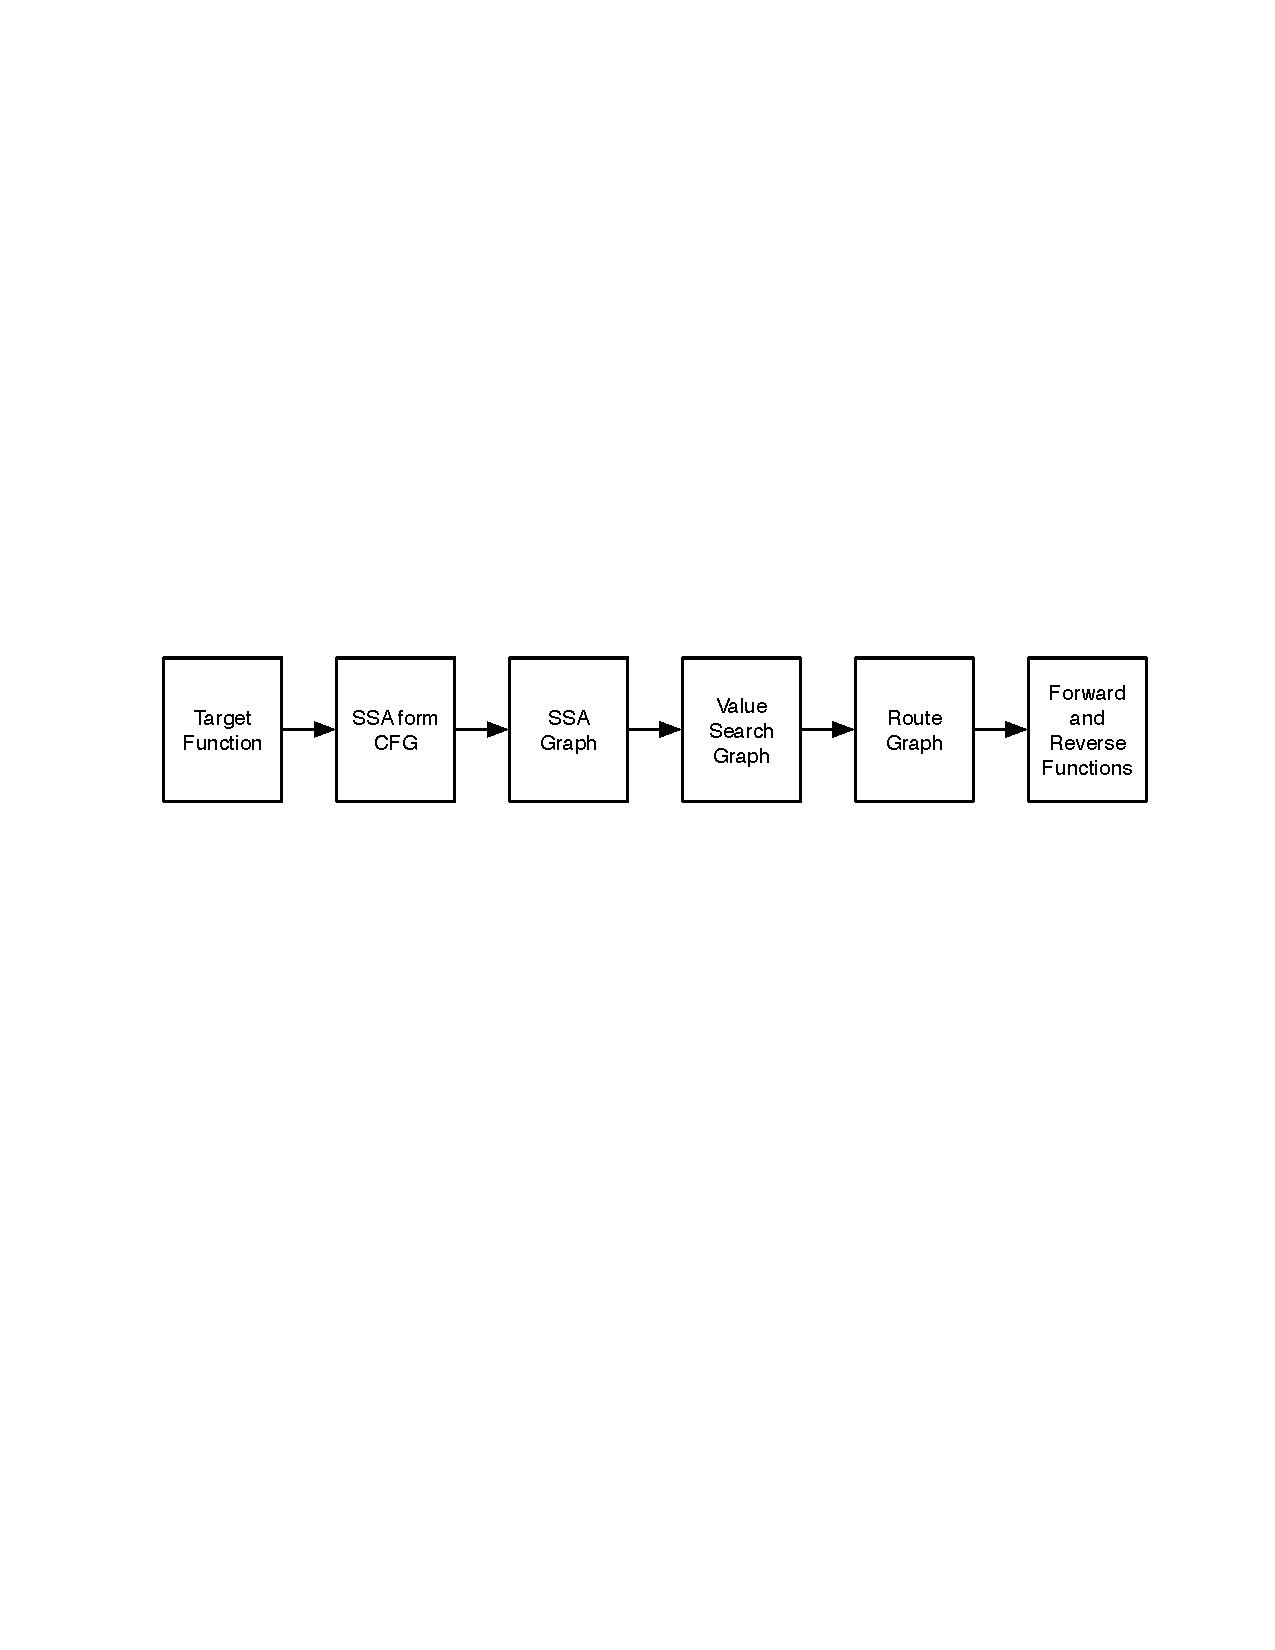
\includegraphics[width=400pt]{figures1/Framework.pdf}
\caption{Overall framework of the inversion algorithm}
\label{fig:framework}
\end{figure}

To restore target values, we will build a graph which shows equality relationships between values. 
We call this graph the \emph{value search graph}, and it is built based on an SSA graph \cite{Alpern1988,Cooper2001}. 
Then a search is performed on the value search graph to recursively find ways to recover the set of target values given the set of available values. 
If there is more that one way to restore a value, we choose the one with the smallest cost. 
The search result is a subgraph of the value search graph which we call a \emph{route graph}. 
For any path, a route graph shows a specific way to recover each target value from available values. 
Finally, the forward and reverse functions are built from a route graph. 
Figure \ref{fig:framework} illustrates this process.

In this section, we will use the example shown in Figure~\ref{fig:code_example} to illustrate our method.


\begin{figure}
\centering
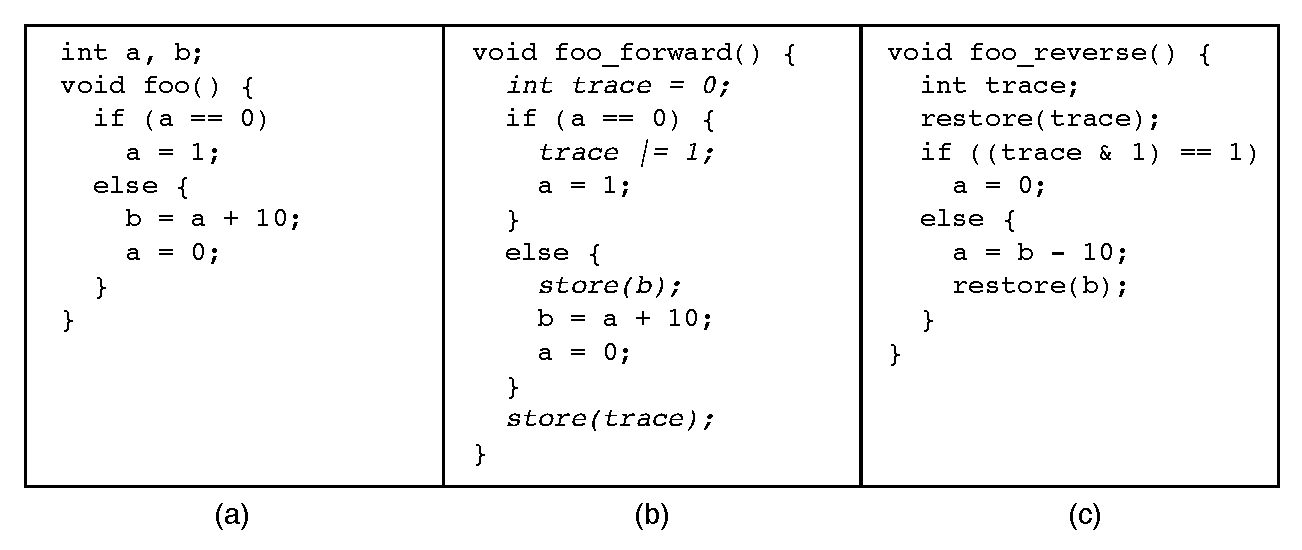
\includegraphics[width=430pt]{figures1/CodeExample.pdf}
\caption{(a) The original function $\quad$ (b) The forward function$\quad$ (c) The reverse function}
\label{fig:code_example}
\end{figure}

\subsection{The value search graph (VSG)}
We first build an SSA graph for the target function.
An SSA graph \cite{Alpern1988,Cooper2001}, built based on SSA form, consists of vertices representing operators, function symbols, or $\phi$ functions, and directed edges connecting uses to definitions of values. It shows data dependencies between different variables. 
The full algorithm for building an SSA graph is presented in \cite{Muchnick}. 
Figure \ref{fig:VSG}(a)(b) show the SSA-transformed CFG and its SSA graph for the function in Figure \ref{fig:code_example}(a). In this example, \texttt{a} and \texttt{b} are two target variables with initial values \texttt{a$_0$} and \texttt{b$_0$}, and final values \texttt{a$_3$} and \texttt{b$_2$}.

\begin{comment}
\begin{figure}
\centering
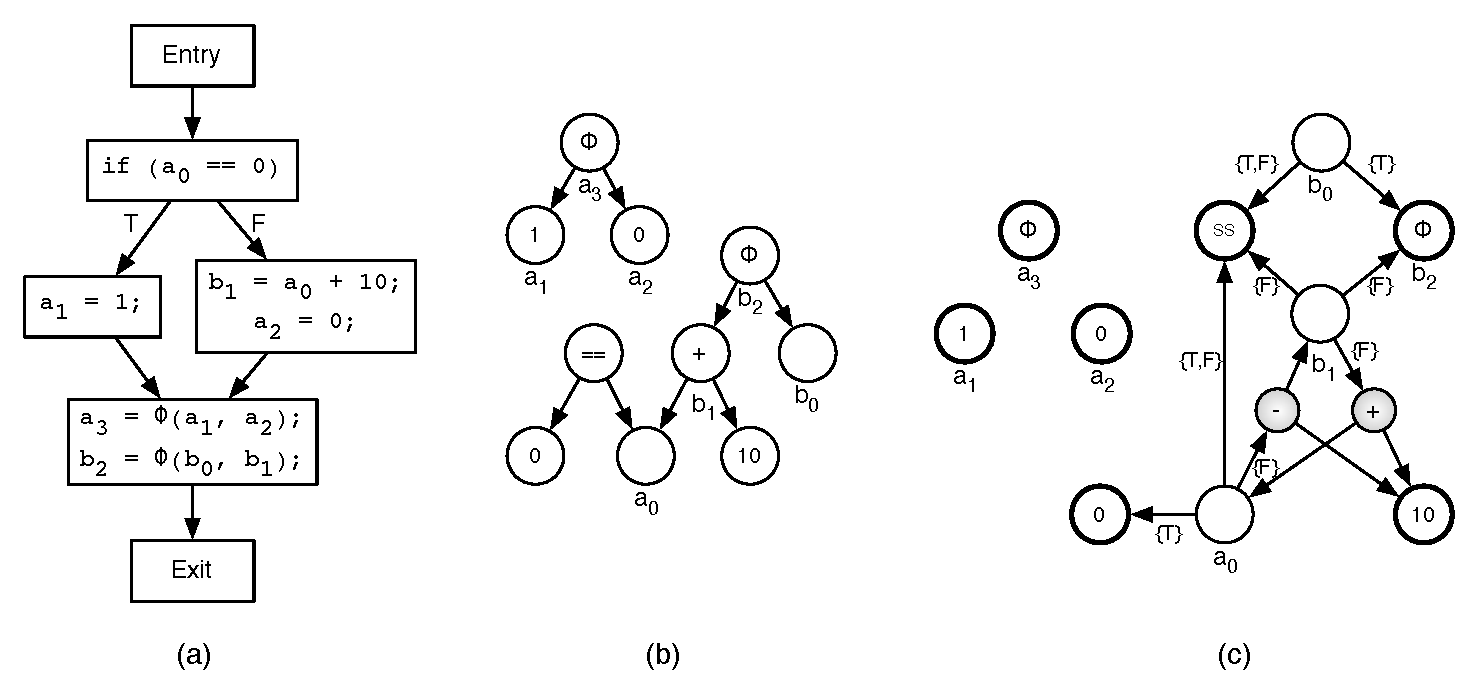
\includegraphics[width=400pt]{figures1/CFG.pdf}
\caption{(a) The SSA-transformed CFG of the function in Figure \ref{fig:code_example}(a)$\quad\quad$ (b) The corresponding SSA graph $\quad\quad$ (c) The corresponding value search graph. Nodes with bold outlines are available nodes; outgoing edges for these nodes are omitted because available nodes need not be recovered. `SS' is the special state saving node. Edges are annotated with their CFG path set.}
\label{fig:VSG}
\end{figure}
\end{comment}

\begin{figure}%
\centering

\begin{subfigure}{0.5\textwidth}
\Drawgraph{
    \node [array,font=\small] (1) at (0,-.5) {\texttt{Entry}};
    \node [array,font=\small] (2) at (0,-2) {\texttt{if (a$_0$ == 0)}};
    \node [array,font=\small] (3) at (-2,-4) {\texttt{a$_1$ = 1;}};
    \node [array,font=\small] (4) at (2,-4)  {
    \parbox{2.7cm}{
    \texttt{b$_1$ = a$_0$ + 10;}\\
      \texttt{a$_2$ = 0;}
    }};
    \node [array,font=\small] (5) at (0,-6) {
    \parbox{3cm}{
    \texttt{a$_3$ = $\phi$(a$_1$, a$_2$);}\\
      \texttt{b$_2$ = $\phi$(b$_0$, b$_1$);}
    }};
    \node [array,font=\small] (6) at (0,-7.5) {\texttt{Exit}};
    \path
    (1) edge [post] (2)
    (2) edge [post] node  [lbl,swap,yshift=-3] {T}(3)
    (2) edge [post]  node  [lbl,yshift=-3] {F}(4)
    (3) edge [post] (5)
    (4) edge [post] (5)
    (5) edge [post] (6)
    ;
}{}{}
\end{subfigure}%
\\
\begin{subfigure}{0.5\textwidth}
\Drawgraph{
    \node [scalar, available, label=below:$a_1$] (a1) at (0,2) {1};
    \node [scalar, available,label=below:$a_2$] (a2) at (2,2) {0};
    \node [scalar, available,label=above:$a_3$] (a3) at (1,3.5) {$\phi$};
    \node [scalar,label=below:$a_0$] (a0) at (4,-2.5) {};
    \node [scalar,available] (10) at (6,-2.5) {10};
    \node [scalar,available] (0) at (2,-2.5) {0};
    \node [scalar, label=above:$b_0$] (b0) at (5,3.5) {};
    \node [scalar, label=right:$b_1$] (b1) at (5,.5) {};
    \node [scalar,available,label=right:$b_2$] (b2) at (6,2) {$\phi$};
    \node [scalar,available] (ss) at (4,2) {SS};
    \node [op] (p) at (5.5,-1) {$+$};
    \node [op] (m) at (4.5,-1) {$-$};
    \path
    (a0) edge [post] node  [lbl] {T,F} (ss)
    (b0) edge [post] node  [lbl,swap] {T,F} (ss)
    (b1) edge [post] node  [lbl, yshift=3,xshift=3] {F} (ss)
    (b0) edge [pre and post] node  [lbl] {T} (b2)
    (b1) edge [pre and post] node  [lbl,swap, yshift=3] {F} (b2)
    (a0) edge [post] node  [lbl] {T} (0)
    (a0) edge [post] node  [lbl,swap, yshift=3,xshift=-3] {F} (m)
    (m) edge [post] node  [lbl] {} (b1)
    (m) edge [post] node  [lbl] {} (10)
    (p) edge [post] node  [lbl] {} (a0)
    (p) edge [post] node  [lbl] {} (10)
    (b1) edge [post] node  [lbl, yshift=-3,xshift=0] {F} (p)
    (a1) edge [pre and post] node  [lbl] {T} (a3)
    (a2) edge [pre and post] node  [lbl,swap] {F} (a3)
    ;
}{}{}
\end{subfigure}%
~
\begin{subfigure}{0.5\textwidth}
\Drawgraph{
    \node [scalar,label=below:$a_0$] (a0) at (4,-2.5) {};
    \node [scalar,available] (10) at (6,-2.5) {10};
    \node [scalar,available] (0) at (2,-2.5) {0};
    \node [scalar, label=above:$b_0$] (b0) at (5,3.5) {};
    \node [scalar, label=right:$b_1$] (b1) at (5,.5) {};
    \node [scalar,available,label=right:$b_2$] (b2) at (6,2) {$\phi$};
    \node [scalar,available] (ss) at (4,2) {SS};
    \node [op] (m) at (4.5,-1) {$-$};
    \path
    (b0) edge [post] node  [lbl,swap] {F} (ss)
    (b0) edge [post] node  [lbl] {T} (b2)
    (b1) edge [post] node  [lbl,swap, yshift=3] {F} (b2)
    (a0) edge [post] node  [lbl] {T} (0)
    (a0) edge [post] node  [lbl,swap, yshift=3,xshift=-3] {F} (m)
    (m) edge [post] node  [lbl] {} (b1)
    (m) edge [post] node  [lbl] {} (10)
    ;
}{}{}
\end{subfigure}%

\caption{(a) The SSA-transformed CFG of the function in Figure \ref{fig:code_example}(a)$\quad\quad$ (b) The corresponding SSA graph $\quad\quad$ (c) The corresponding value search graph. Nodes with bold outlines are available nodes; outgoing edges for these nodes are omitted because available nodes need not be recovered. `SS' is the special state saving node. Edges are annotated with their CFG path set.}
\label{fig:VSG}
\end{figure}





A \emph{value search graph} enables efficient recovery of values by explicitly representing equality relationships between values. 
Unlike an SSA graph, operation nodes are separated from value nodes in the value search graph, since their treatment is different for recovering values.
An edge connecting two value nodes $u$ and $v$ implies that $u$ and $v$ have the same value. 
%However, the equality of two values may only be true for certain CFG paths; hence each edge in a VSG is annotated with the set of CFG paths to which it applies.
An edge from value node $u$ to an operation node $op$ means that  $u$ is equal to the result of evaluating $op$ with its operands. 
To recover the value associated with node $v$, we can recursively search the graph starting at $v$.  

We attach a set of CFG paths to each edge in a value search graph, meaning the edge is applicable only if one of the CFG paths in that set is selected in the original function.
For operation nodes in the SSA graph, let the set of paths attached to each outgoing edge be the CFG paths for which the corresponding operation is executed. 
Similarly, for $\phi$ nodes, each reaching-definition edge should be annotated with all CFG paths for which the corresponding reaching definition reaches the $\phi$ function. 
We will describe an implementation of the path set representation later.

During the execution of the forward function, once a variable is assigned with a new value, its previous value may be destroyed and cannot be retrieved. To guarantee that a search in the value search graph can always restore a value, we introduce special \emph{state saving edges}. 
The idea behind these edges is that each value may be recovered by storing it during the forward execution. 
Whenever a state saving edge appears in the search results, the forward function is instrumented to save the corresponding value. 
The path set associated with a state saving edge for a value node $v$ is the set of all paths that include $v$'s definition. All state saving edges point to a unique \emph{state saving node}. %since it is not necessary to create a state saving node for every state saving edge.

\begin{comment}
\begin{figure}
\center{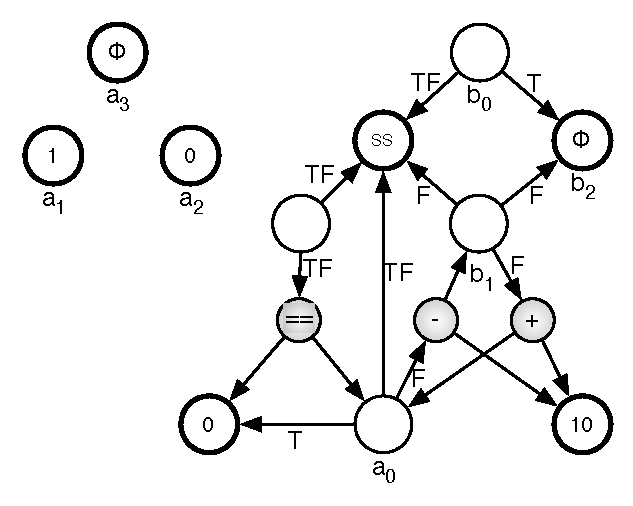
\includegraphics[width=160pt]{figures1/VSG.pdf}}
\caption{The value search graph for the function in Figure \ref{fig:code_example}(a). All available nodes are shown in bold. The label on edges from an operation node is only shown on the in-edge.}
\label{fig:VSG}
\end{figure}
\end{comment}

We apply the following rules to convert an SSA graph into a value search graph:
\begin{itemize}
	\item For simple assignment $v = w$, there is a directed edge from $v$ to $w$ in the SSA graph. 
	Since we can retrieve $w$ from $v$, add another directed edge from $w$ to $v$ with the same path set.

	\item A $\phi$ node in the SSA graph has several outgoing edges connecting all its possible definitions. 
	For each of those edges, add an opposite edge with the same path set. 
	
	\item For each operation node in the SSA graph, split it into an operation node and a value node, with an edge from the value node to the new operation node. 
	The new operation node takes over all outgoing edges, and the value node takes over all incoming edges. 
	
	\item If an equality operation (\texttt{==}) is used as a branching predicate and its outcome is true, we know that the two operands are equal.
	Therefore, we add edges from each operand to the other, with a path set for the edge equal to the path set of the \emph{true} CFG edge out of the branch. 
	We add the edges analogously for a not-equal operation (\texttt{!=}), but with the path set from the \emph{false} side of the branch.
	
	\item For every value that is not available, insert a state saving edge from the corresponding value node to the state saving node. 
\end{itemize}

\paragraph{Lossless operations} For certain operations, such as integer addition and exclusive-or, we can recover the value of an operand given the operation result and the other operand. For example, if $a=b+c$, we can recover $b$ given $a$ and $c$. For each such lossless operation, insert new operation nodes that connect its result to its operands, allowing the operands to be recovered from the result. The new nodes are added according to the following rules:

%\footnote{Assume there is no type conversion. Type conversion can be treated as a special operation, which we won't discuss here.}

\begin{center}
\begin{tabular}{|c|c|c|}
  \hline
  Operation name & Original operation & New operations added \\
  \hline \hline 
  Negation & \texttt{a = -b} & \texttt{b = -a} \\
  \hline    
  Bitwise not& \texttt{a = \textasciitilde b} & \texttt{b = \textasciitilde a} \\
  \hline
  Logical not& \texttt{a = !b} & \texttt{b = !a} \\
  \hline    
  Increment & \texttt{++a} & \texttt{--a} \\
  \hline    
  Decrement & \texttt{--a} & \texttt{++a} \\
  \hline
  Integer addition & \texttt{a = b + c} & \texttt{b = a - c} \\
  {} & {} & \texttt{c = a - b} \\
  \hline
  Integer subtraction & \texttt{a = b - c} & \texttt{b = a + c} \\
  {} & {} & \texttt{c = b - a} \\
  \hline
  Bitwise exclusive-or & \texttt{a = b \textasciicircum{ }c} & \texttt{b = a \textasciicircum{ }c} \\
  {} & {} & \texttt{c = a \textasciicircum{ }b} \\
  \hline
\end{tabular}
\end{center}

\begin{comment}
\begin{figure}
\center{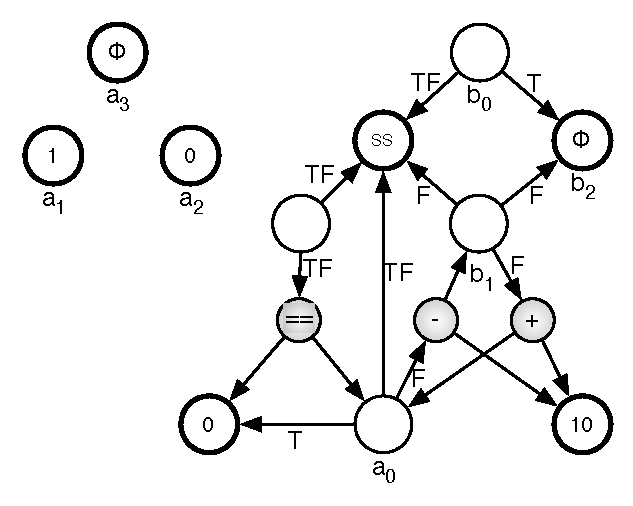
\includegraphics[width=160pt]{figures1/VSG.pdf}}
\caption{The value search graph for the function in Figure \ref{fig:code_example}(a). All available nodes are shown in bold. The label on edges from an operation node is only shown on the in-edge.}
\label{fig:VSG}
\end{figure}
\end{comment}

There are two special types of nodes in a value search graph: \emph{target nodes} are value nodes containing target values, and \emph{available nodes} are value nodes containing available values plus the state saving node.
As an optimization, we never create any outgoing edges for an available node. Figure \ref{fig:VSG}(c) shows the value search graph built for the code in Figure \ref{fig:code_example}(a). 
The available nodes are shown with a bold outline.
Since the function only has two paths, we use labels `T' and `F' to represent the CFG paths passing through the true and false body in the target function, respectively. 
The `--' operation node connecting $a_0$ to $b_1$ and the constant value `10' is generated from the `+' operation. 
The edge from $a_0$ to `0' for the path `T' is added based on the fact that $a_0 = 0$ on that path.
The `SS' node in the graph is the state saving node, and all unavailable nodes are connected to it. 
From the value search graph, we can find two valid ways to restore $b_0$ for the path `T': $b_0$ to SS node and $b_0$ to $b_2$. 
Obviously the second one is better since it avoids a state saving operation, and this better selection will be produced from the search algorithm described later.


\subsection{The route graph (RG)}
\label{sec:route-graph}

A \emph{route graph} is a subgraph of a value search graph connecting all target nodes to available nodes. Each route graph represents one way to restore the target values, and there may exist many valid route graphs for the same set of target values.
Edges in the route graph may have different path sets than the corresponding edges in the value search graph. 
For each edge $e$ in a route graph, let $P(e)$ denote the set of CFG paths that the edge is annotated with.
The following properties guarantee that the route graph properly restores all target values:

\begin{enumerate}[I)]

\item Let $\mathcal{U}$ be the set of all CFG paths. Then, for each target node $t$, 
	$$\bigcup_{\mathit{out} \in \text{OutEdges}(t)}P(\mathit{out}) \quad = \quad \mathcal{U} $$ 
	\label{rg-property-1}

\item For each node $n$ that is neither a target node nor an available node,
	$$\bigcup_{\mathit{out} \in \text{OutEdges} (n)} P(out) = \bigcup_{\mathit{in} \in \text{InEdges} (n)}P( \mathit{in} )$$ 

\item For each value node $n$, given any two outgoing edges $n\to p$ and $n\to q$, $P(n\to p) \cap P(n\to q) = \emptyset$ 

\item If $e$ is a route graph edge and its corresponding edge in the value search graph is $e'$, then $P(e) \subseteq P(e')$
	\label{rg-property-4}

\item For each directed cycle with edges $e_1 \dots e_n$,  $\quad \bigcap_{i=1}^n{P(e_{i})} = \emptyset$
	\label{rg-property-5}

\end{enumerate}

Property I specifies that each target value is recovered for every CFG path. 
Property II means that each value is recovered exactly for the paths for which it is needed.
Property III requires that for each CFG path, there is at most one way to recover a value. 
Property IV requires that the set of CFG paths associated with an edge in the route graph is a subset of the CFG paths originally associated with that edge in the value search graph. Finally, property V forbids self-dependence: restoring a value cannot require that value. 

\begin{figure}[htb]
\center{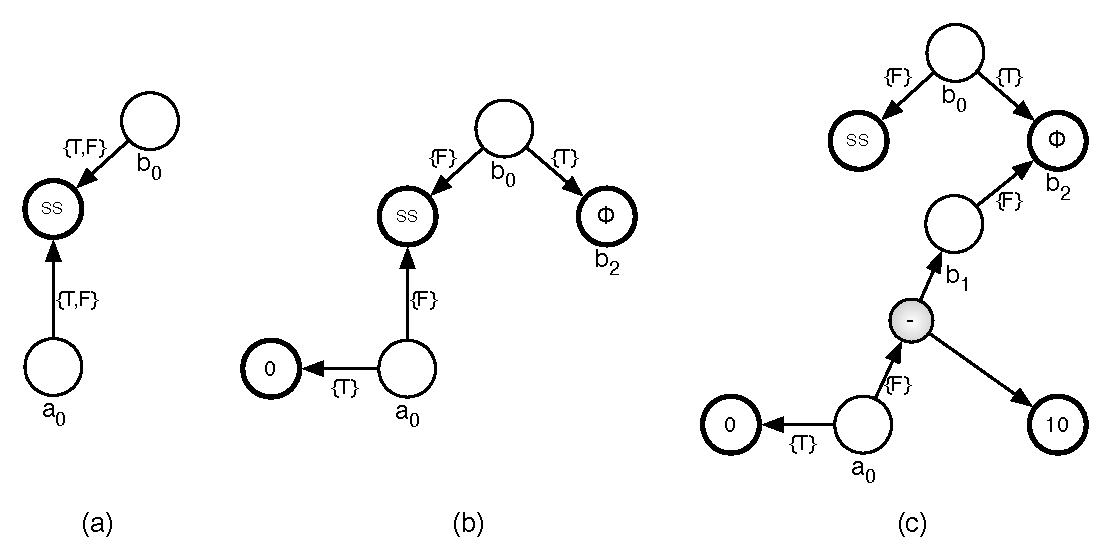
\includegraphics[width=400pt]{figures1/RG.pdf}}
\caption{Three different route graphs for the target values $\text{a}_{\text{0}}$ and $\text{b}_{\text{0}}$ given the the value search graph in Figure \ref{fig:VSG}(c). %While all three route graphs restore the target values, they have different costs.
}
\label{fig:RG}
\end{figure}

Figure \ref{fig:RG} shows three valid route graphs for the value search graph in Figure \ref{fig:VSG}. 
Route graph \ref{fig:RG}(a) only includes state saving edges. 
Route graph \ref{fig:RG}(b) takes advantage of the fact that for the `T' path the values of both \texttt{a$_0$} and \texttt{b$_0$} are known; it only uses staving for the `F' path. 
Route graph \ref{fig:RG}(c) improves upon route graph \ref{fig:RG}(b) by recomputing \texttt{a$_0$} as \texttt{b$_1$-10} for the CFG path `F'; state saving is only applied to \texttt{b$_0$} for path `F'.



\subsection{Searching the value search graph}

\subsubsection{Costs in route graphs}
As we have seen in Figure \ref{fig:RG}, there may be multiple valid route graphs that recover the target values, but with different overheads. 
In order to choose the route graph with the smallest overhead, we must define a cost metric.

Generally, there are two kinds of overhead in forward and reverse functions: execution speed and additional memory usage; we only consider the storage costs.
State saving contributes the most to the overhead memory usage and it also significantly affects the running time of both forward and reverse functions. 
Storing the path taken during forward execution is the other factor that contributes to memory usage; this overhead is bounded and is the same for all route graphs, so we exclude it from our cost estimate. 
With each state saving edge in the value search graph, we associate a cost equal to the size of the value that must be saved; other edges have cost 0.
%All other edges in the VSG have a small cost $\varepsilon$ associated with them, the technical reasons for which we will elucidate later. 
The cost of a route graph for a specific CFG path is the sum of the cost of those edges whose annotated path sets include that CFG path.

In Figure \ref{fig:RG}, suppose the cost to store and restore either \texttt{a} or \texttt{b} is $c$, the following table shows the cost of three route graphs for each CFG path.
% (here we ignore $\varepsilon$ just for clarity). 
Obviously the third route graph is the best one.

\begin{center}
\begin{tabular}{|c|c|c|c|}
%\begin{tabular}[c]{| c || m{1cm} | m{1cm} | m{1cm} |}
  \hline
  CFG path & route graph (a) & route graph (b) & route graph (c) \\
  \hline\hline
  T & $2c$ & $0$ & 0 \\
  \hline
  F & $2c$ & $2c$ & $c$ \\
  \hline
\end{tabular}
\end{center}

We have defined the cost of a single CFG path; however, a route graph may have different costs for different CFG paths.
When searching the value search graph, we would like to treat groups of CFG paths that share some edges in the route graph together, rather than performing a full search for each CFG path.
For this reason, the search algorithm partitions the CFG paths into disjoint sets of paths that have equal cost and we save the cost for each set of paths independently. 
In our search algorithm, we denote the costs of a route graph $r$ as $r.$costSet.
\[ r.\text{costSet} = \{ \langle P_{i}, c_{i} \rangle | P_{i}\text{ is a set of CFG paths and } c_{i} \text{ is the cost}\} \]
%\[P_{i} \cap P_{j} = \emptyset \quad \text{ if } i \neq j \]



\begin{algorithm}
\footnotesize
\label{algorithm:search}
\LinesNumbered
\DontPrintSemicolon

\SetKwData{NewCond}{newPaths}
\SetKwData{condition}{pathSet}
\SetKwData{cond}{paths}
\SetKwData{vertex}{target}
\SetKwData{edge}{edge}
\SetKwData{edges}{edges}
\SetKwData{edgeb}{e}
\SetKwData{target}{target}
\SetKwData{visited}{visited}
\SetKwData{subRoute}{newRoute}
\SetKwData{subGraph}{subGraph}
\SetKwData{route}{route}
\SetKwData{cost}{cost}
\SetKwData{eCopy}{eCopy}
\SetKwData{target}{target}
\SetKwData{subRoutes}{subRoutes}
\SetKwData{result}{resultRoute}
\SetKwData{costSet}{costSet}
\SetKwInOut{Input}{Initial input}

\SetKwFunction{OutEdges}{OutEdges}
\SetKwFunction{SearchSubRoute}{SearchSubRoute}
\SetKwFunction{SearchRoute}{SearchRoute}
\SetKwFunction{UpdateConditions}{ChooseMinimalCosts}

\Input{The search start point \vertex, with \cond $= \emptyset$, \visited $= \emptyset$}




\BlankLine
\SearchSubRoute{\vertex, \cond, \visited} \;
\Begin{
  \result $\leftarrow \emptyset$,  \subRoutes $\leftarrow \emptyset$ \;
  \If{\vertex is an operation node}{
      \ForEach{\edge $\in$ \OutEdges{\vertex}}{
          \lIf{\edge.\target $\in$ \visited}{\Return $\emptyset$\;}
          \subRoute $\leftarrow$ \SearchSubRoute{\edge.\target, \cond, \visited}\; 
          \lIf{\subRoute $= \emptyset$}{\Return $\emptyset$\;}
          add \edge and \subRoute to \result \;
      }
      \Return \result \;
  }
  \If{\vertex \mbox{is available}}{
      add \vertex to \result \;
      add $\langle \cond, 0 \rangle$ to \result.\costSet \;
      \Return \result \;
  }
  \ForEach{\edge $\in$ \OutEdges{\vertex}}{
    \lIf{\edge.\target $\in$ \visited}{continue}  
    \BlankLine
    \NewCond $\leftarrow$ \edge.\condition $\cap$ \cond\; 
    \lIf{\NewCond $=  \; \emptyset$}{continue} 
    \BlankLine

    \subRoute $\leftarrow$ \SearchSubRoute{\edge.\target, \NewCond, \visited$\cup \; \{\vertex\}$}\;
 
    add \edge with paths \NewCond to \subRoute\;
    \lForEach{$\langle \cond, \cost \rangle$ in $\subRoute.\costSet$}{
        \cost += \edge.\cost\;
    }
        \lForEach{\route in \subRoutes}{
    \UpdateConditions{\route, \subRoute}\;
    }


      add \subRoute to \subRoutes \;

  }
  add \vertex to \result \;
  \ForEach{\route in \subRoutes}{
      \lIf{$\route.\condition \ne \emptyset$}{
          add \route to \result \;
      }
  }
  \Return \result \;
}

\SetKwData{routea}{route1}
\SetKwData{condition}{pathSet}
\SetKwData{routeb}{route2}
\SetKwData{edge}{edge}
\SetKwData{graph}{routeGraph}
\SetKwData{conda}{paths1}
\SetKwData{condb}{paths2}
\SetKwData{costa}{cost1}
\SetKwData{costb}{cost2}
\SetKwData{paths}{paths}
\SetKwData{cost}{cost}

\BlankLine
\BlankLine
\UpdateConditions{\routea, \routeb} \;
\Begin{
    \lIf{\routea.\condition $\cap$ \routeb.\condition  $ = \emptyset$}{
        return\;
    }
    \ForEach{$\langle \conda, \costa \rangle$ in \routea.\costSet}{
        \ForEach{$\langle \condb, \costb \rangle$ in \routeb.\costSet}{
            \lIf{\conda $\cap$ \condb $= \emptyset$}{
                continue\;
            }
            \If{\costa $>$ \costb} {$\conda \leftarrow \conda - \condb $\;
            Remove (\conda $\cap$ \condb) from all edges of \routea \;}
            \Else{$\condb \leftarrow \condb - \conda $\;
            Remove (\conda $\cap$ \condb) from all edges of \routeb \;}
        }
    }
    \routea.\condition $ = \bigcup_{\langle \paths, \cost \rangle \in \routea.\costSet} \paths $ \;
    \routeb.\condition $ = \bigcup_{\langle \paths, \cost \rangle \in \routeb.\costSet} \paths $
}

\caption{Searching for a route graph in a value search graph}

\end{algorithm}

\subsubsection{Search algorithm}
Our search algorithm should aim to find a route graph that has the minimum cost for each path. 
Theoretically, however, searching for a minimal route graph is an NP-complete problem. 
To make the problem tractable, we apply the heuristic of finding a route graph for each target value individually; the individual route graphs are then merged into a route graph that restores all the target values. 
Similarly, in order to recover the value of a binary operation node, we recover each of the two operands independently and then combine the results. 

The pseudocode for our heuristic search algorithm is presented in Algorithm \ref{algorithm:search}. 
The {\tt SearchSubRoute} function returns a route graph given a target node, the paths for which that node must be restored, and the set of value nodes visited so far.
The algorithm explores all ways to recover the current node by calling itself recursively on all the nodes that are directly reachable from the current node; available nodes are the base case.
Lines 5--10 handle recovering the values of operation nodes. 
In order to recover the value of an operation node, each of its operands must be recovered.
Lines 11--14 return a trivial route graph for available nodes, with a cost of 0. 
The remaining body of the algorithm (lines 15--27) handles recovering a value node that is not available.
Each of the out-edges of the target node may be used to recover its value for the CFG paths associated with that edge; these edges are explored in the {\tt for}-loop in lines 15--23.
The variable {\tt newPaths} on line 17 represents the set of paths that we are both interested in and are associated with the current edge. 
In line 19, we recursively find a route graph that recovers the target value by recovering the target of the current outgoing edge.
Lines 21--22 update the cost sets of the new route graph; if it provides a lower cost for some CFG path than the solutions found so far, the partial results are modified so that each CFG path is restored with the cheapest route graph.
Finally, the route graph from line 19 is added to the list of partial results (line 23). 
After all out-edges of the target node have been explored, the partial results are merged into a single route graph and returned (lines 24--27).
Note that it is unnecessary to check whether the target node has been successfully recovered, since the state saving edge always provides a valid route graph for the node. 
Figure \ref{fig:RG}(c) shows the route graph produced by the algorithm when searching the value search graph from Figure \ref{fig:VSG}(c).

The search algorithm enforces properties \ref{rg-property-1}--\ref{rg-property-4} from section \ref{sec:route-graph} during its execution.
To make sure that the search result does not contain cycles (property \ref{rg-property-5}), we record which value nodes are already in the route using a set \texttt{visited} in Algorithm \ref{algorithm:search}. 
This alone is not sufficient to guarantee that the result is acyclic, for there may be two different paths with identical cost to recover a single value node. 
If one way is chosen to recover a value node $v$ during path of the search, and then later $v$ is recovered differently for the same CFG path, a cycle may form.
To prevent this situation from occurring, we always traverse out-edges in the same order of line 19 of Algorithm \ref{algorithm:search}; the first route graph with the smallest cost is chosen. In addition, two paths coming from two different value nodes may also form a cycle when all costs on edges of the cycle are 0. We eliminate this possibility by replacing 0 by a small cost $\varepsilon$.
% Do we really need to have epsilon for correctness? It seems that the above condition is sufficient to guarantee correctness

\begin{comment}
\paragraph{Extensions} Adding constraints during the search could produce different inversion strategies. 
For example, putting only state saving edges to the route graph will produce the same result as checkpointing.
Including state saving edges and phi edges (edges incident to a phi node) results in the incremental state saving, where a variable is saved only for the paths for which it is modified. 
\end{comment}

\subsection{Instrumentation and Code generation}

\subsubsection{Representing CFG path sets}

Our search algorithm relies on efficiently computing intersection, union, and complement of CFG path sets, as well as testing whether the set of paths is empty; for this reason we suggest implementing the set representations as bit vectors. 
Ball and Larus \cite{Ball1996} present an path profiling method in which each path is given a number from 0 to $m-1$, where $m$ is the count of the CFG paths. 
We use their algorithm to number each path, and for each path we associate exactly one bit in the bit vector used to represent a path set.
%Algorithm \ref{algorithm:findPaths} illustrates how to use depth-first search on the CFG to find the set of paths that correspond to each CFG edge; the search is initially invoked with \texttt{FindCfgPaths(Entry, 0)}.

\begin{comment}

\begin{algorithm}
\label{algorithm:findPaths}
\DontPrintSemicolon
\caption{Finding the set of paths passing through each CFG edge}



\SetKwFunction{findCfgPaths}{FindCfgPaths}
\SetKwFunction{OutEdges}{OutEdges}

\SetKwData{node}{node}
\SetKwData{edge}{edge}
\SetKwData{target}{target}
\SetKwData{pathIndex}{pathIndex}
\SetKwData{exitNode}{\textbf{Exit}}
\SetKwData{pathsHere}{pathsFound}
\SetKwData{pCount}{count}

\BlankLine
\findCfgPaths{\node, \pathIndex} \;
\Begin{
	\lIf{\node == \exitNode}
	{
		\Return 1 \;
	}
	\pathsHere $\leftarrow$ 0 \;

	\ForEach{\edge $\in$ \OutEdges{\node}}
	{
		\pCount $\leftarrow$ \findCfgPaths{\edge.\target, \pathIndex} \;
		Add paths \pathIndex through (\pathIndex + $\pCount - 1$) to \edge \;
		\pathsHere $\leftarrow$ \pathsHere + \pCount \;
		\pathIndex $\leftarrow$ \pathIndex + \pCount \;
	}
	\Return{\pathsHere} \;
}

\end{algorithm}

\end{comment}

\subsubsection{Recording CFG paths}
\label{sec:encoding-paths}
\begin{comment}
We can encode a path with a path number as above, and checking if a path set represented by a bit vector contains a path is also fast. However, the length of a bit vector equals the number of CFG paths, which can be large. Further, we will see later that each branch in the reverse function is translated from the path set on a route graph edge. If there are $m$ CFG paths in the target function, and $n$ distinct path sets used to generate the predicates in the reverse function, then we need $m\times n$ bits of static memory in the reverse function! %Another problem comes that we may also need the condition  in the forward method for the state saving statement. 
Our solution is using another method to encode CFG paths. We will see that a path set can be transformed to a set of new representations, from which we can build more efficient predicates in the reverse function.
\end{comment}

We need to store path information in a way that allows us to efficiently record the CFG path taken (for forward execution), and to efficiently check if the path matches a given set of CFG paths attached to a route graph edge (for reverse execution). 
However, if we encode each path using its path number, then examining whether a path is a member of a set is inefficient.
% (we don't want each path set represented by a bit vector to appear in the reverse code, which may take too much memory). 
Instead we  %employ another approach to encoding paths, and 
use a bit vector to record the CFG path, in which each bit represents the outcome of a branching statement. 
%We will see later that this new path encoding will result in quite efficient comparisons in the reverse execution.
Since this method is similar to \emph{bit tracing}\cite{Ball1994}, we call this bit vector a \emph{trace}.
Note that two branches may share the same bit if they cannot appear in the same path. Thus, the number of bits required to store the path taken is equal to the largest number of branches that appear on a single CFG path.
Algorithm \ref{algorithm:conditions} calculates bit-vector position for each branch node accordingly.

\begin{algorithm}
\label{algorithm:conditions}
\DontPrintSemicolon

\SetKwData{vertex}{u}
\SetKwData{vertexa}{v}
\SetKwData{vertexb}{w}
\SetKwData{mask}{mask}
\SetKwFunction{bitPosition}{position}
\SetKwFunction{maxVal}{max}

\BlankLine
\BlankLine
    \ForEach{CFG node \vertex in reverse topological order}{
        \uIf{\vertex is a leaf node}{
            \bitPosition{\vertex} $\leftarrow$ -1 \;
        }
            \uElseIf{\vertex is a branch node}{
                \tcc{$\vertex\to\vertexa$ and $\vertex\to\vertexb$ are its two out-going edges} 
                \bitPosition{\vertex} $\leftarrow$ \maxVal{\bitPosition{\vertexa}, \bitPosition{\vertexb}} + 1\;
            }
            \Else{ 
                \tcc{$\vertex\to\vertexa$ is its out-going edge} 
                \bitPosition{\vertex} $\leftarrow$ \bitPosition{\vertexa} \;
            }         
    }

\caption{Generating the bit position for each branch node.}
\end{algorithm}

In the forward function, we use an integer as the bit vector to record all predicate results\footnote{Potentially we could omit recording predicates that do not affect the reverse function.}. 
Let \texttt{trace} be the variable recording a trace, initialized to zero; then the true edge of each branch node $v$ is instrumented with the statement \footnote{We use several operators in C/C++ syntax here and below, which includes bitwise OR operator \texttt{|}, bitwise AND operator \texttt{\&}, bitwise left shift operator  \texttt{<<}, equal to operator \texttt{==}, and logical OR operator \texttt{||} .}
$$ \texttt{trace = trace  | (1 << $\mathit{position(v)}$)}; $$ 
where $\mathit{position(v)}$ is calculated by Algorithm \ref{algorithm:conditions}. 
The variable \texttt{trace} is stored at the end of the forward function and restored at the beginning of the reverse function. 
Note that we can further optimize the instrumentation by moving a trace updating operations downward through the CFG and merging them.
%The Ball and Larus maximal spanning tree method for calculating edges to instrument is also applicable \cite{Ball1996}. 



In the reverse function, we must test if \texttt{trace} matches the path sets that appear on route graph edges. We start with transforming each path in the set into a trace (the trace for each path can be computed by the same means as recording a trace in the forward function).
Then, checking if a path set contains a path represented by \texttt{trace} is done by comparing it to each trace. 
Suppose a path set containing two paths is transformed into two traces \texttt{01101} and \texttt{01001}. Instead of comparing \texttt{trace} to each of them as:
$$ \texttt{if (trace == 01101 || trace == 01001)} $$ 
we can simplify this predicate by using a mask \texttt{11011} on \texttt{trace}:
$$ \texttt{if ((trace \& 11011) == 01001)} $$ 

The combined trace for \texttt{01101} and \texttt{01001} is \texttt{01$\times$01}, where $\times$ denotes that the bit does not matter. 
Given a set of traces, we can combine pairs repeatedly to reduce the size of the set.
This greatly reduces the complexity of the branching statements in the reverse code. 
\begin{comment}

Each CFG path is induced by a sequence of branches that must be either true or false; we can build the corresponding mask by setting 0 or 1 in the position corresponding to each branch. 
Some elements of the mask representing a CFG path may be $\times$, which signifies that the outcome of the corresponding branch does not affect whether the path is taken or not. 
Algorithm \ref{algorithm:computeMasks} computes the path mask associated with each CFG path; it is initially invoked as \texttt{ComputePathMasks(Entry, 0, $\times$$\times$$\dots$$\times$$\times$)}. 
Note that the indices computed for each path by Algorithm \ref{algorithm:computeMasks} match those computed by Algorithm \ref{algorithm:findPaths}; in fact, these two algorithms can be merged into one. 


\begin{algorithm}
\label{algorithm:computeMasks}
\DontPrintSemicolon
\caption{Finding mask corresponding to each CFG path}

\SetKwFunction{computePathMasks}{ComputePathMasks}
\SetKwFunction{OutEdges}{OutEdges}

\SetKwData{node}{node}
\SetKwData{edge}{edge}
\SetKwData{target}{target}
\SetKwData{pathIndex}{pathIndex}
\SetKwArray{currentMask}{currentMask}
\SetKwData{exitNode}{\textbf{Exit}}
\SetKwData{pathsHere}{pathsFound}
\SetKwData{pCount}{count}
\SetKwFunction{bitPosition}{position}
\SetKwData{edgeLabel}{label}

\BlankLine
\computePathMasks{\node, \pathIndex, \currentMask} \;
\Begin{
	\If{\node = \exitNode}
	{
		\currentMask is the mask for the path \pathIndex \;
		\Return 1
	}
	\pathsHere $\leftarrow$ 0 \;

	\ForEach{\edge $\in$ \OutEdges{\node}}
	{
		\If{\edge is labeled} 
		{
			\currentMask{\bitPosition{\node}} $\leftarrow$ 
			$\begin{cases} 0 \text{ if } \edge.\edgeLabel = F \\ 1 \text{ if } \edge.\edgeLabel = T \end{cases}$
		}
		\pCount $\leftarrow$ \computePathMasks{\edge.\target, \pathIndex, \currentMask} \;
		\pathsHere $\leftarrow$ \pathsHere + \pCount \;
		\pathIndex $\leftarrow$ \pathIndex + \pCount \;
	}
	\Return{\pathsHere} \;
}

\end{algorithm}

In order to test the recorded path against a set of CFG paths, we may test the mask of the path against each of the masks in the set. 
For example, we can test for the mask 00$\times$10 with \texttt{((cfgmask \& 11011) == 00010)}.
To make these checks more efficient, however, we may merge multiple CFG paths into a single mask.
For example, if the masks for two paths are $0011$ and $0111$, we can test for either path with the mask 0$\times$11. 

\end{comment}


Algorithm \ref{algorithm:mergeMasks} starts out with all traces corresponding to a set of CFG paths and merges them into a minimal set of traces that can be used to test membership in the set. 
The intuition behind Algorithm \ref{algorithm:mergeMasks} is that if the traces are sorted so that bit $i$ is the least significant bit, the traces that are identical to each other except for bit $i$ will be adjacent. 
However, if we are careful we don't have to pay the full sorting cost for each bit $i$. 
If the traces are sorted when their bits are considered in the order $b_{1} b_{2} \dots b_{i - 1} \quad b_{k} b_{k - 1} \dots b_{i} $ and we want to sort them according to the bit order $b_{1} b_{2} \dots b_{i - 2} \quad b_{k} b_{k - 1} \dots b_{i - 1} $, we need only sort each sequence of the trace for which bits 1 through $(i-2)$ are identical. 
For each such sequence, there are at most three sorted subsequences, indexed by bit $b_{i-1}$; these can be merged in linear time (similarly to mergesort).
If we use a linear-time sort, such as radix sort, for the first iteration, the overall runtime of Algorithm \ref{algorithm:mergeMasks} is $O(k n)$, where $n$ is the size of the path set.


\begin{algorithm}
\label{algorithm:mergeMasks}
\DontPrintSemicolon
\caption{Merging a set of path traces}

\SetKwFunction{mergePathMasks}{MergePathTraces}

\SetKwArray{masks}{traces}
\SetKwData{bitSize}{k}
\SetKwData{index}{i}
\SetKwData{maskIndex}{j}

\SetKw{KwDownTo}{down to}

\SetKwFunction{length}{Length}

\mergePathMasks{\masks} \;
\Begin{
	\tcc{Each trace has \bitSize "bits", and each bit is 0, 1, or $\times$}
	\tcc{Bits are numbered ascendingly; e.g. $m = b_{1} b_{2} \dots b_{k}$}

	\For{\index $\leftarrow$ \bitSize \KwDownTo $1$}
	{
		\tcc{Note: for \index = k, the bit ordering is $m = b_{1} b_{2} \dots b_{k}$}
		Sort \masks, where trace bits are ordered $b_{1} b_{2} \dots b_{i - 1} \quad b_{k} b_{k - 1} \dots b_{i} $ \;
		
		\For{\maskIndex $\leftarrow$ 2 \KwTo \length{\masks}}
		{
			\If{ \masks{\maskIndex$-\;1$} and \masks{\maskIndex} match except for bit \index}
			{
				set bit \index to $\times$ for  \masks{\maskIndex$-\;1$} \;
				delete \masks{\maskIndex}
			}
		}
	}
	

	
}

\end{algorithm}

After the merge, if we have $n$ traces $t_1,...,t_n$ for a path set, the resulting predicate would be:
$$\texttt{if ((trace \& $mask_1$) == $obj_i$ || ... || (trace \& $mask_n$) == $obj_n)$}$$
For each trace $t_i$, $mask_i$ is obtained by setting all bits which are $\times$ in $t_i$ to 0 and others to 1, and $obj_i$ equals $mask_i$ \texttt{\&} $t_i$.



\subsubsection{Inserting state saving statements}
\label{sec:state-saving}
The other instrumentation in the forward function are state saving statements, which are inserted according to the state saving edges in the route graph. 
For each state saving edge in the route graph, suppose the variable to store is $var$ and the path set on this edge is $P$. 
Our task is finding one or several locations to store $var$ according to the path set $P$, ensuring that $var$ is only saved once for each CFG path in $P$. 

To find such locations, we first compute the corresponding path traces $T$ of $P$ from Algorithm \ref{algorithm:mergeMasks}. 
For each trace in $T$, we traverse the CFG from the entry. 
When we reach a branch node, check the corresponding bit in the trace: fall through the true edge if the bit is 1, false edge if the bit is 0. 
If the bit is $\times$, the traversal forks and that bit is assigned to 0 and 1 respectively forming two new traces; and for each concretized trace the descent continues. 
The descent stops immediately when all bits which are not checked in the trace are $\times$. 
After this process, we obtain one or more locations where the descent has stopped. 
%This is not clear. It's better to leave it out than to have it be confusing
%If the tracings from two traces stop at the same location, we then combine them again (since they may be forked from one trace previously). 
%In each maximal basic block in which each location resides, 
In each location we find a point where the definition of $var$ is reachable and a state saving statement is inserted there. 
However, it is possible that the path set containing the paths passing through this location is larger than the one on which the state saving is needed. 
In this case, we guard the state saving statement with a branch whose predicate corresponds to the trace at this location.



\subsubsection{Building a CFG for the reverse function}
We build the CFG for the reverse function from a route graph; the reverse CFG is acyclic and each path in it must obey the data dependencies represented in the route graph.
Each outgoing edge from a value node in the route graph will be translated to a statement in the reverse function. 

There could be a large number of correct reverse CFGs for a route graph, resulting in different control flows and different numbers of branches. 
%Without the runtime information such as profiling data, it is difficult to determine with one is the best with respect to the performance. 
We choose to build a structured CFG to simplify the translation to source code. 
We also attempt to minimize the number of predicates in the CFG. 

There are three kinds of statements that can be generated from a route graph:
\begin{itemize}
	\item An operator node with its operands and result induces an operation statement,  such as \texttt{a = b + c}.
	\item An edge with value nodes as both ends induces an assignment statement.
	\item An edge pointing to the SS node induces an value restoration statement.
\end{itemize}

%For the purposes of code generation, we shall refer to an operation node together with its incoming and outgoing edges as an operation (hyper)edge, which is a special edge with one source and one or more targets.
%With this convention, each statement corresponds to one ``edge'' in the route graph.

The statements generated from route graph edges retain the path sets attached to the corresponding edges.
We build basic blocks of statements that all share the same path sets, and insert branches so that each basic block is executed when the corresponding path is taken in the forward function. 
While enforcing the path set constraints ensures correct control flow, producing correct data flows depends on the order in which statements are inserted in the CFG.
Note that a route graph corresponds to explicit data dependencies, and for each CFG path in the forward function it is acyclic due to property \ref{rg-property-5} from section \ref{sec:route-graph}. 
Hence, if we order statements in the reverse topological order of the route graph edges, dataflow dependencies are correctly maintained.

\begin{algorithm}
\footnotesize
\label{algorithm:reverse-cfg}
\LinesNumbered
\DontPrintSemicolon
\caption{Generating a CFG for the reverse function from a route graph.}


\SetKwData{bb}{b}
\SetKwData{bone}{b1}
\SetKwData{btwo}{b2}
\SetKwData{stmts}{pendingStmts}
\SetKwData{bbs}{openBlocks}
\SetKwData{s}{s}
\SetKwData{cond}{pathSet}
\SetKwData{cp}{pathSetPairs}
\SetKwData{edge}{edge}
\SetKwData{valNode}{valNode}
\SetKwData{RG}{routeGraph}
\SetKwData{CFG}{cfg}
\SetKwData{source}{source}
\SetKwData{availNode}{availNode}
\SetKwFunction{GenerateReverseCFG}{GenerateReverseCFG}
\SetKwFunction{GetStatements}{BuildReadyStatements}
\SetKwFunction{InEdges}{InEdges}

\SetKwFunction{BuildBB}{BuildBasicBlock}
\SetKwData{entry}{entry}

\BlankLine
\GenerateReverseCFG{\RG}\\
\Begin
{
	\CFG $\leftarrow \emptyset$, \stmts $\leftarrow \emptyset$, \bbs $\leftarrow \emptyset$, \cp $\leftarrow \emptyset$\; 
	\lForEach{\valNode in \RG}
	{
		\valNode.\cond $\leftarrow \emptyset$\;
	}
	\ForEach {available node \availNode in \RG}
	{
		\GetStatements{\availNode, $\mathcal{U}$, \stmts} \;
	}
	\CFG.\entry $\leftarrow$ \BuildBB{$\mathcal{U}$} \;
	%Create a new basic block with path set $\mathcal{U}$ as the entry of the CFG and add it to \CFG and \bbs\;
    
	\While{$\stmts \neq \emptyset$}
	{
		\uIf{$\exists \s \in \stmts, \bb \in \bbs$, and $\s.\cond = \bb.\cond$}
		{
			Append \s to \bb\;
			\valNode $\leftarrow$ the source node of the edge that generated \s \;
			 \GetStatements{\valNode, \s.\cond, \stmts}\;
 		}
		\uElseIf{$\exists \s \in \stmts, \bb \in \bbs$, and \s.\cond $\subset$ \bb.\cond}
		{
			Append to \bb a branch, with the predicate generated from \s.\cond\;
			\bone $\leftarrow$ \BuildBB{\s.\cond} \;
			Append \s to \bone\;
			\btwo $\leftarrow$ \BuildBB{$\bb.\cond - \s.\cond$} \;
			%Create two new basic blocks $\bone$ and $\btwo$ with path set \s.\cond and $\bb.\cond - \s.\cond$ respectively, and add them to \CFG and \bbs\;
			Insert into \CFG edges from \bb to \bone and \btwo with labels \textit{true} and \textit{false} \;
			Add $\langle \bone.\cond, \btwo.\cond \rangle$ to \cp\;
			\bbs $\leftarrow \; \bbs - \{ \bb \}$ \;
			%Remove  \bb from \bbs\;
			\valNode $\leftarrow$ the source node of the edge that generated \s \;
			\GetStatements{\valNode, \s.\cond, \stmts}\;
 		}
		\ElseIf{$\exists \bone, \btwo \in \bbs$, and $\langle \bone.\cond, \btwo.\cond \rangle \in \cp$}
		{
			\bb $\leftarrow$ \BuildBB{\bone.\cond $\cup$ \btwo.\cond} \;
			%Create basic block \bb, $\bb.\cond = \bone.\cond \cup \btwo.\cond$, and add \bb to \CFG and \bbs\;
			Insert into \CFG two edges, from \bone and \btwo to \bb\;
			\cp $\leftarrow \; \cp - \{ \langle \bone.\cond, \btwo.\cond \rangle \}$ \;
			%Remove $\langle \bone.\cond, \btwo.\cond \rangle$ from $\cp$\;
			\bbs $\leftarrow \; \bbs - \{ \bone, \btwo \}$ \;
			%Remove \bone and \btwo from \bbs\;
			\lIf{$|\bbs| = 1$}{break}
		}
	}
	\Return{\CFG}
}

\BlankLine

\SetKwData{availablePathSets}{nodeAvailablePaths}

\GetStatements{\valNode, \availablePathSets, \stmts}\\
\Begin
{
	\valNode.\cond $\leftarrow$ \valNode.\cond $\cup$ \availablePathSets \;
	\ForEach{\edge $\in$  \InEdges{\valNode}}
	{
		\If{\edge.\cond $\subseteq$ \valNode.\cond}
		{
			\uIf{\edge.\source is an operation node}
			{
				Set \edge to be a available for \edge.\source \;
				\If{all operands of \edge.\source are available}
				{
					Add to \stmts the statement for for \edge.\source, with path set \edge.\cond \;
				}
			}
		\Else
		{
			Add to \stmts the statement for \edge, with path set \edge.\cond \;
		}}
	}
}
\BlankLine

\BuildBB{\cond}
\Begin
{
	Build an empty basic block \bb and attach path sets \cond to it. \;
	\CFG $\leftarrow$ \CFG $\cup$ \{ \bb \}, $\quad$
	\bbs $\leftarrow$ \bbs $\cup$ \{ \bb \} \;
	\Return{ \bb } \;
}

\end{algorithm}

Algorithm \ref{algorithm:reverse-cfg} shows how to build a CFG for the reverse function. 
We keep a set of basic blocks, \texttt{openBlocks}, to which new statements can be appended.  
We also maintain a set of statements, \texttt{pendingStmts}, whose data dependencies have been satisfied, but which have not yet been inserted in the CFG.
Each basic block has an associated path set; these are the paths in the forward function for which the corresponding basic block in the reverse function should execute.
Similarly, each statement has a set of paths from the forward function. 
If there is a pending statement and an open basic block whose path sets match, we simply append the statement to the basic block.
When a statement is inserted into the CFG, the data dependencies of new statements may now be satisfied; we call the function \texttt{BuildReadyStatements} to generate the statements that are now valid for insertion. 
If there is no pending statement whose path set matches the path set of an open basic block, we must insert or join a branch in the CFG.
When a branch is inserted, two new basic blocks are created and the basic block containing the branch is closed. 
%The branch predicate is generated from the path set mask and from the CFG path recorded during forward execution, as described in section \ref{sec:encoding-paths}.
When a branch is joined, the joined basic blocks are closed and a new open basic block is created.
%Finally, if all open basic blocks have path sets that are too specific to insert any statement, we must join the two sides of a branch together.

Note that it is possible that the instrumentation to the forward function brings additional implicit data dependencies. 
For example, if stack is used for state saving the order of values popped in the reverse function should be opposite of the order of pushes in the forward function. 
In this case, we can order those state saving statements in \texttt{pendingStmts} according to the order in which values are pushed.


\subsubsection{Generating code} 
The forward function is generated by copying the target function and adding state saving and control flow instrumentation (section \ref{sec:encoding-paths}). 
The reverse function is translated from the CFG built by Algorithm \ref{algorithm:reverse-cfg}. 
Translating a structured CFG to source code is straightforward. 
Since each variable in the reverse CFG is in SSA form, we can use the versioned name during code generation. 
Because our framework generates source code that is later compiled with another compiler, the redundant variables will be optimized away; the only drawback of this approach is readability.
If readability is an issue, we can compute data dependencies in the reverse CFG and then remove versions attached to variables where this does not affect data dependencies.
After version removal, we would also remove self-assignment statements such \texttt{a = a}.
Figures \ref{fig:code_example}(b) and \ref{fig:code_example}(c) show the generated forward and reverse functions from the code in Figure~\ref{fig:code_example}(a).



\section{Experiment results}

We have implemented the framework in our C/C++ source-to-source translator Backstroke based on the ROSE compiler. 
Since this paper focuses on arbitrary control flows and basic operations with only scalar data types, instead of trying to reverse real-world code, which usually includes function calls, non-scalar data types, aliasing, etc., we employ some representative synthetic benchmarks to illustrate the power of our algorithm. Those benchmarks are listed below.

\newcommand{\NoBranch}{\textbf{NoBranch}\xspace}
\newcommand{\Branchesa}{\textbf{Branches1}\xspace}
\newcommand{\Branchesb}{\textbf{Branches2}\xspace}
\newcommand{\Branchesc}{\textbf{Branches3}\xspace}
\newcommand{\Loopa}{\textbf{Loop1}\xspace}
\newcommand{\Loopb}{\textbf{Loop2}\xspace}
\newcommand{\Asn}{\textbf{Assignment}\xspace}
\newcommand{\Inc}{\textbf{Increment}\xspace}
\newcommand{\CSS}{\textbf{CSS}\xspace}
\newcommand{\ISS}{\textbf{ISS}\xspace}
\newcommand{\RCC}{\textbf{RCC}\xspace}

\begin{itemize}

\item \NoBranch: A variable is modified in the function.


%\item \textbf{Unstructured}: A simple unstructured code with two predicates and two side effects.

\item \Branchesa: There are many CFG paths in the function and only one variable is modified on one path.

\item \Branchesb: There are many CFG paths in the function and on each path a distinct variable is modified.

\item \Branchesc: There are many CFG paths in the function and a variable is modified up to three times on some paths and is not modified on other paths.

%\item \textbf{EarlyExits}: Several early exits exist in several different branches.

\item \Loopa: A loop in which a variable is modified. The loop is intended to have many iterations at runtime.
\item \Loopb: A loop containing a simple branch and two variables are modified in the true and false body respectively. The loop is intended to have many iterations at runtime.
%\item \textbf{LoopWithEarlyExit}: A loop containing an early exit inside with one side effect.


\end{itemize}

In addition, each benchmark has two versions in which every variable is modified differently: in the first one, each variable is modified by an assignment; the other one modifies each variable using an increment operation (\texttt{++}) so that the assignment can be reversed trivially. 
We denote those two versions by \Asn and \Inc. 

We compare our method\footnote{Note that for loops we use the non-loop solution as defined in section \ref{sec:loops}.} to three other approaches commonly employed in the OPDES community to implement rollback:

\begin{itemize}
\item \CSS: Copy state saving. Every target variable is stored at the beginning of the forward function and restored in the reverse function. Here we only store the variables that are potentially modified.
\item \ISS: Incremental state saving. A variable is stored only the first time it is modified. 
This technique is traditionally implemented by storing the variable's address along with its value, so one can check if the variable is already stored.

\item \RCC: Reverse C compiler~\cite{Carothers1999} is a syntax-directed incremental inversion translator (see section \ref{sec:related-work}). 
\end{itemize}

We count the maximum and minimum memory used for state saving. 
The memory used to record the control flows outside of loops (including the counter recording the number of iterations in a loop) is ignored because it does not scale with the size of the program state. 
Figure \ref{fig:charts} shows the experiment results, in which (a) and (b) are maximum and minimum memory usage for all benchmarks of the \Asn version, and (c) and (d) are of the \Inc version. The height of each column represents the memory usage. 

From the result we can see for most benchmarks Backstroke is the most efficient, which is because our method integrates the advantages from both incremental reverse execution and incremental state saving. 
\ISS stores the address of every variable which introduces a large overhead if the address's size is comparable to that of a value's (for scalar data) meanwhile we utilize the CFG path to ensure each variable is stored only once, with much less overhead.
\ISS outperforms \CSS when there are many variables which are potentially modified but only a small number of them are modified during each execution (see Figure \ref{fig:charts} \Branchesb). That is why incremental state saving performs very well when each event only modifies a small portion of the whole state.


\newcommand{\FigSize}{320pt}

\begin{figure}%
\centering
%
\begin{subfigure}{\textwidth}
\centering
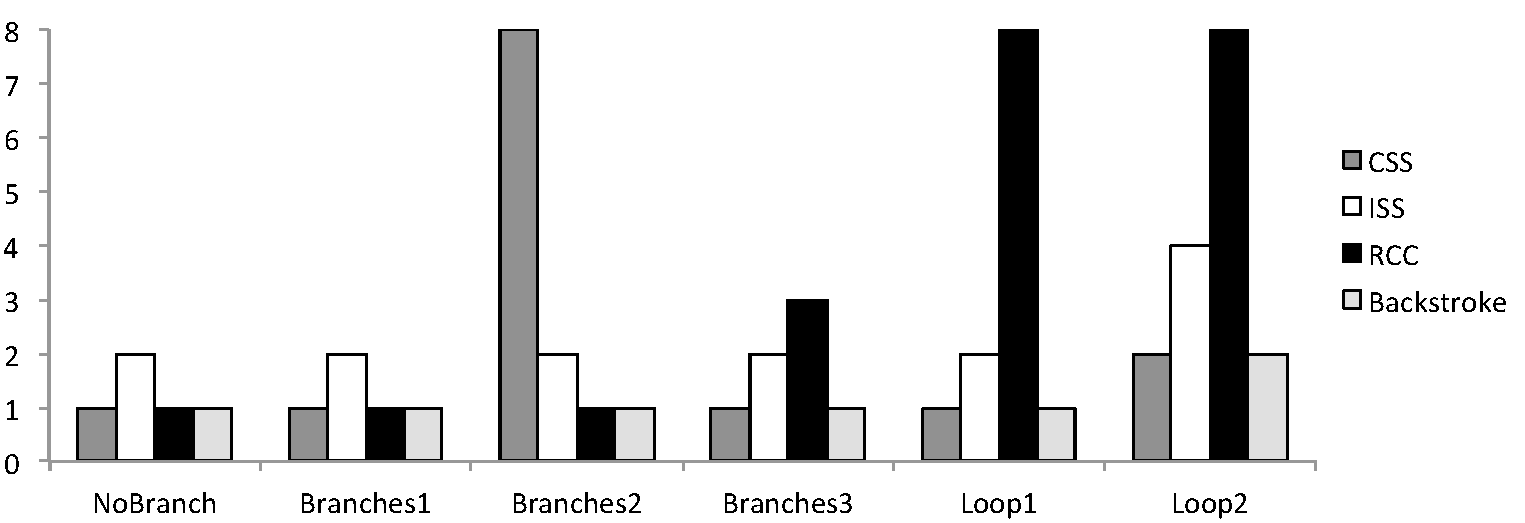
\includegraphics[width=\FigSize]{figures1/chart1.pdf}
\caption{Maximum memory usage of \Asn}
%\label{fig:code_example}
\end{subfigure}
\\
\begin{subfigure}{\textwidth}
\centering
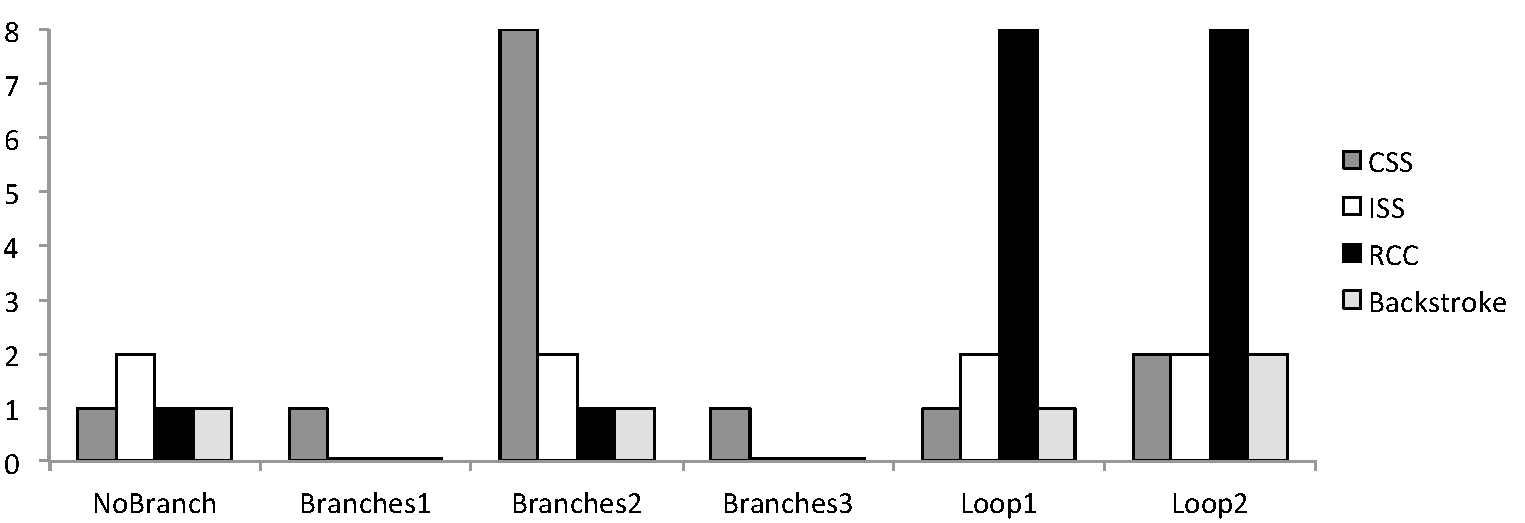
\includegraphics[width=\FigSize]{figures1/chart2.pdf}
\caption{Minimum memory usage of \Asn}
\end{subfigure}
\\
\begin{subfigure}{\textwidth}
\centering
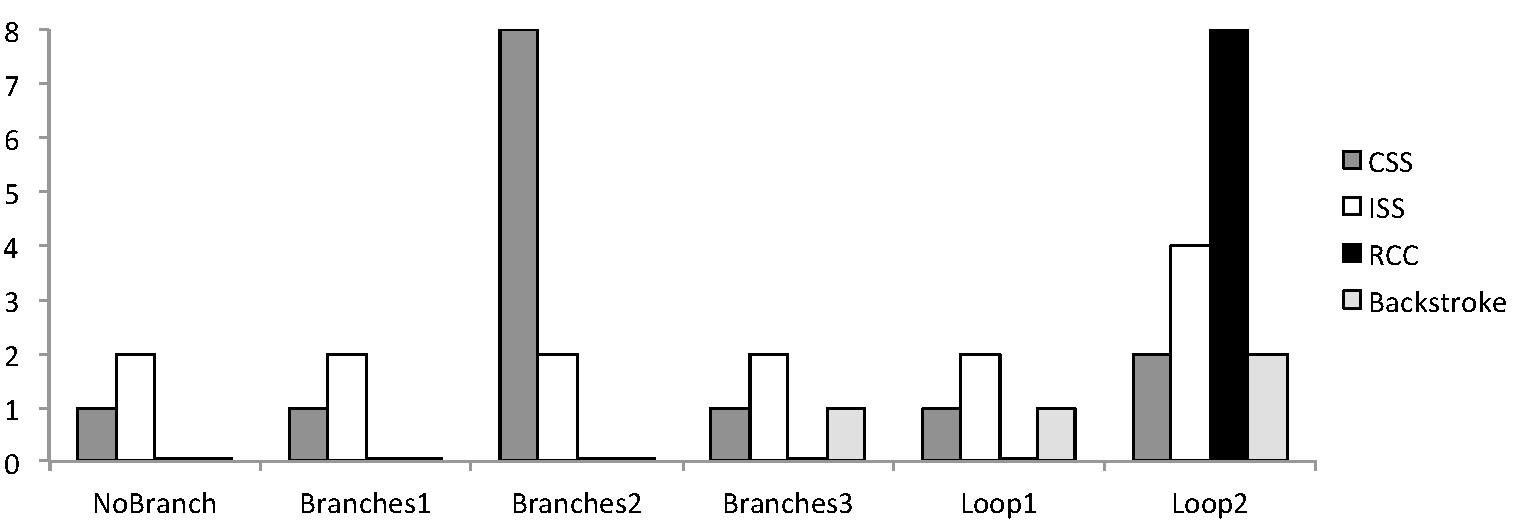
\includegraphics[width=\FigSize]{figures1/chart3.pdf}
\caption{Maximum memory usage of \Inc}
\end{subfigure}
\\
\begin{subfigure}{\textwidth}
\centering
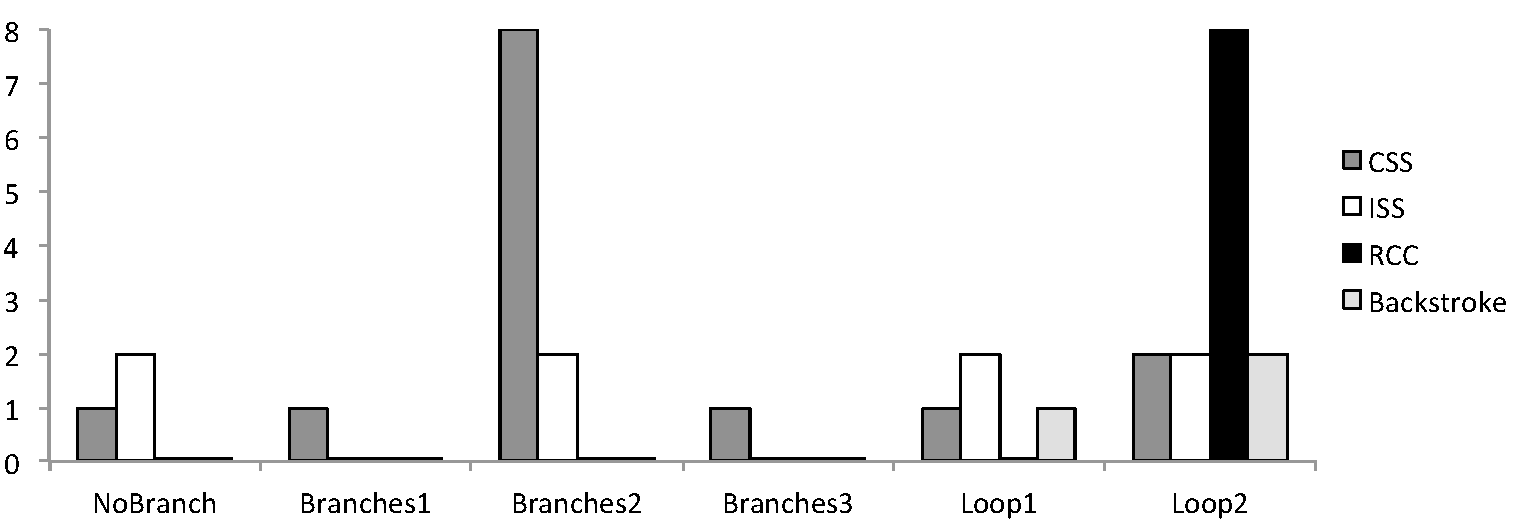
\includegraphics[width=\FigSize]{figures1/chart4.pdf}
\caption{Minimum memory usage of \Inc}
\end{subfigure}

\caption{Experiment results}
\label{fig:charts}
\end{figure}

From comparing the results from Figure \ref{fig:charts} (a)(b) and (c)(d), it is clear that the reverse execution approaches can save much memory. 
But the amount of benefit from reverse execution is determined by the number of opportunities for reverse computation. 
For programs that do not have many lossless operations such as \texttt{++} and \texttt{+=}, state saving still plays an important role in their inversions.

We must be very cautious when reversing a loop. If the loop solution is applied, we have to determine if storing control flow information is worth it or not.
The result of \Loopb from \RCC shows that if the number of iterations is large, storing control flows is not good idea. 
Saving state inside a loop normally is not a wise choice, as the result of \Loopa+ \Asn from \RCC show.




%Table 1 shows three examples, each including an original function and its generated forward and reverse function from our algorithm. For all of them, both \texttt{a} and \texttt{b} are target variables. The \texttt{cond1} and \texttt{cond2} are predicates whose content we don't care. In the first function \texttt{foo1()}, \texttt{a} is modified either \texttt{cond1} or \texttt{cond2} is true. If \texttt{cond1} and \texttt{cond2} are both true, it is not necessary to store \texttt{a} twice. Therefore, in the forward function, when \texttt{cond2} is true, we check if \texttt{a} is once stored or not to avoid multiple stores for the same value. This is exactly the same as incremental state saving, which is the best strategy here. The second function \texttt{foo2()} contains unstructured code.  The restoration of \texttt{a} and \texttt{b} does not need any state saving.  The function \texttt{foo3()} has a loop with an early exit. 

\begin{comment}

\begin{table}
\begin{center}
\small
\begin{tabular}{| m{3cm} | m{4.2cm} | m{4.2cm} |}
  \hline
  Original function & Forward function & Reverse function \\
  \hline \hline 
\begin{verbatim}
void foo1() {
  if (cond1)
    a = 0;
  if (cond2)
    a = 1;
} 
\end{verbatim}
  & 
\begin{verbatim}
void foo1_forward() {
  int bitvec = 0;
  if (cond1) {
    bitvec |= 2;
    store(a);
    a = 0;
  }
  if (cond2) {
    bitvec |= 1;
    if (bitvec & 3 == 1)
      store(a);
    a = 1;
  }
  store(bitvec);
} 
\end{verbatim}
   &
\begin{verbatim}
void foo1_reverse() {
  int bitvec;
  restore(bitvec);
  
  if (bitvec & 3 == 1)
    restore(a);
  else {
    if (bitvec & 2 == 2)
      restore(a);
  }
} 
\end{verbatim} 
\\
  \hline    
\begin{verbatim}
void foo2() {
  if (cond1) {
    ++a;
    if (cond2)
      goto L;
  }
  else
L:  ++b;
}
\end{verbatim}
&
\begin{verbatim}
void foo2_forward() {
  int bitvec = 0;
  if (cond1) {
    bitvec |= 2;
    ++a;
    if (cond2) {
      bitvec |= 1;
      goto L;
    }
  }
  else
L:  ++b;
  store(bitvec);
}
\end{verbatim}
&
\begin{verbatim}
void foo2_reverse() {
  int bitvec;
  restore(bitvec);
  
  if (bitvec & 2 == 2)
    --a;
  if (bitvec & 3 == 3 ||
      bitvec & 2 == 0)
    --b;
} 
\end{verbatim}
\\
  \hline    
\begin{verbatim}
void foo3() {
  while (cond1) {
    ++a;
    if (cond2)
        return;
    ++b;
  }
}
\end{verbatim}
&
\begin{verbatim}
void foo3_forward() {
  int bitvec = 0, k = 0;
  while (cond1) {
    ++a;
    if (cond2) {
      bitvec |= 1;
      return;
    }
    ++b;
    ++k;
  }
  store(k);
  store(bitvec);
}
\end{verbatim}
&
\begin{verbatim}
void foo3_reverse() {
  int bitvec = 0, k = 0;
  restore(bitvec);
  restore(k);
  
  if (bitvec & 1 == 1)
    --a;
  while (k--) {
    --b;
    --a;
  }
}
\end{verbatim}
\\
\hline
\end{tabular}
\end{center}
\caption{Three examples with generated forward and reverse functions.}
\end{table}

\end{comment}

%\subsection{Function Calls}
%For input only parameters of a function, if it is needed by the reverse function, it can be stored either by caller or by callee. Saving by caller may provide several ways to recover that value, and saving by callee may save that value conditionally.







%============================================================
\section{Handling programs with loops}
\label{sec:scalar-loops}
\newcommand{\pVSG}{\ensuremath{G_P}\xspace}
\newcommand{\lVSG}{\ensuremath{G_L}\xspace}

Unmodified, the method described above cannot handle loops for two key reasons.
%first, it brings cyclic paths, but our prior analysis only rely on acyclic path as the condition of each equality
%
First, a loop results in cyclic paths in the CFG, whereas our prior analysis relies on paths being acyclic.
%
Acyclic paths make it easy to check that the reverse program restores any desired input value no matter what path the forward program takes.
%
Secondly, our prior VSG and RG cannot represent loop control structure.
Therefore, it is simply not possible to synthesize, for example, a loop in the reverse code from the RG.
Nevertheless, we \emph{can} reuse most of the prior method by decomposing the problem suitably.
In particular, we keep the basic framework of ``SSA to VSG to RG.''
Our extension replaces SSA with a loop-enabled variant, and then extends our VSG and RG representations and algorithms to deal with cycles, thereby addressing the two aforementioned issues.
%However, there are some special steps to build the VSG for the program with loops, and the searching rule should also be updated.

Let us first assume that each loop to be reversed is a single-entry, single-exit while loop (we will explain what is a while loop later).
We explain in Section~\ref{sec:other-loops} how to convert other kinds of loops into this form.
We also assume that each loop must terminates at run-time so that we can always get an output.
Given an input while loop, there are three steps to build a VSG.
%
\begin{enumerate}

\item We temporarily collapse each while loop into a single abstract node in the CFG, thereby creating a logically loop-free CFG from which we can build a VSG by directly applying our prior method.
This ``transformation'' is for program analysis purposes only. 
We denote this loop-collapsed VSG by \pVSG.
%forming a loop-free program, and we build the VSG for it. 
%Note that this VSG only contains the input and output of each loop, but doesn't contain any value defined inside of the loop.

\item Similarly, we directly apply our prior method to build a VSG for each loop \emph{body}, which may be treated as another loop-free program.
(If the body contains nested loops, these are similarly collapsed as in Step 1 above.)
%This new VSG connects all input and output of the loop body, but doesn't contain the input and output of the loop. 
Note that path information in these loop body VSGs are local to the loop body.
We denote this VSG for the loop body by \lVSG.

\item At this point, \pVSG and \lVSG are disconnected.
Therefore, we introduce new special edges to connect them, thereby resulting in a single connected VSG.
These connecting edges are a new type of edge and constitute the main extension to our prior VSG in order to support loops.
The new edges connect each input (or output) of a loop to the input (or output) of the loop's body.
%Doing so makes it possible to retrieve the input or output of the loop through the \lVSG, thereby a loop will be generated in the reverse program.
These new edges serve as markers: when we search the VSG and produce an RG containing these edges, then we know we need to synthesize a loop.

\end{enumerate}
%
Since Steps 1 and 2 use our prior VSG construction, we need not discuss them further here.
What changes is the third step, as detailed below, including new VSG searching rules and new procedures for synthesizing loops from the search result (i.e., the RG). %We first deal with while loops then other loops.
Because state saving in a loop is very expensive, we won't consider it in a loop. Moreover, it suffices for us to deal with a single loop without nested loops, which can be handled in the same way recursively.

%Then the question is how can we connect the VSG for the whole program after reducing all loops and VSGs for loop bodies, and let the search freely traverse them to get the final VG. 


%However, in the VSG, there is no connection between the input values and output values for each loop. Therefore, our next step is building the connections between those values. We can treat each loop as another program, but we can also treat the loop body as another program. Assume this is no other loops in the loop body, so that the loop body as its own is a loop-free program which we can handle using our prior method. The third step is, how to build the special relations between the input of the loop and input of the loop body, and the output of the loop and output of the loop body. 

%To reverse a program with loops, the basic idea is similar to that for loop-free programs, but with special manipulations. From the view of the CFG, if we can reduce the loop into a single node with the same input and output, the program will turn into loop-free and will be handled in the previous way. Now what is new is how to build the VSG connecting the input and output of the loop. what we want to Specifically, the VSG built for a loop should show relationships between the input and output of the loop, and during the search if we can find a way from an input to an output or from an output to an input, we can rebuild another loop from this result producing desired values. 




%When we build a value search graph for a program without loops, each value node does contain a distinct value. However, if there is a loop, variables modified in the loop are defined more than once. Even in SSA form, a versioned variable cannot represent a single value. 

%Note that above we require that the loop has single entry and single exit, which is because such a loop has a unique input and output for each variable. 
 %In this section, we first consider a special single-entry single-exit loop: a while loop, and for other loops we will do a transformation on them on the IR level which separates the last iteration\footnote{Here we define an iteration as a control flow path from the entry of the loop header back to the same point or to the entry of an exit of the loop, and each iteration can only contain the loop header once. Hence each loop has at least one iteration at runtime.} from others. All iterations besides the last one have a single entry and a single exit, which are both the loop header, and hence can form a while loop. The last iteration will not belong to the loop and can be combined to the control flows outside of the loop.
%Consequently, we are able to handle all loops.



%Given a loop, a natural idea to get its inverse is building another loop whose body is the inverse of the body of the original loop, and those two loops should have the same number of iterations at runtime, as shown in \cite{Hou2012}, . However, there exist two problems for this approach: first, in practice, a loop may have several exits, and they may connect different control flows outside of the loop, which is difficult to reverse. %For example, consider the possibility of a reverse loop with more than one entry. 
%not have the form \texttt{while(C) S;}, where there is no side effect in \texttt{C}. Most imperative languages allow side effect existing in \texttt{C} above, and they also provide keywords allowing early exit (like \texttt{break}, \texttt{goto}, and \texttt{return} in C/C++), which results in several exits in a loop. 
%Second, if the input and output of a loop are S and T respectively, sometimes we don't want the T and S to be the input and output of the inverse of the loop, but subsets of them. To solve the first problem, we first discuss how to deal with a while loop, a special loop with single exit. For other loops we will do a transformation on them on the IR level which separates the last iteration from others, which guarantees that each iteration except the last one has single entry and single exit. To solve the second problem, we integrate the value search graph of the loop to the whole program then let the search algorithm select the input and output. 

%Our discussion of loops only considers natural loops with only one entry; loops with more than one entry are quite rare in practice and can be transformed into natural loops \cite{Muchnick}. %In this section we first deal with a standard while loop, then other loops. 


\begin{figure}%[htb]
\center{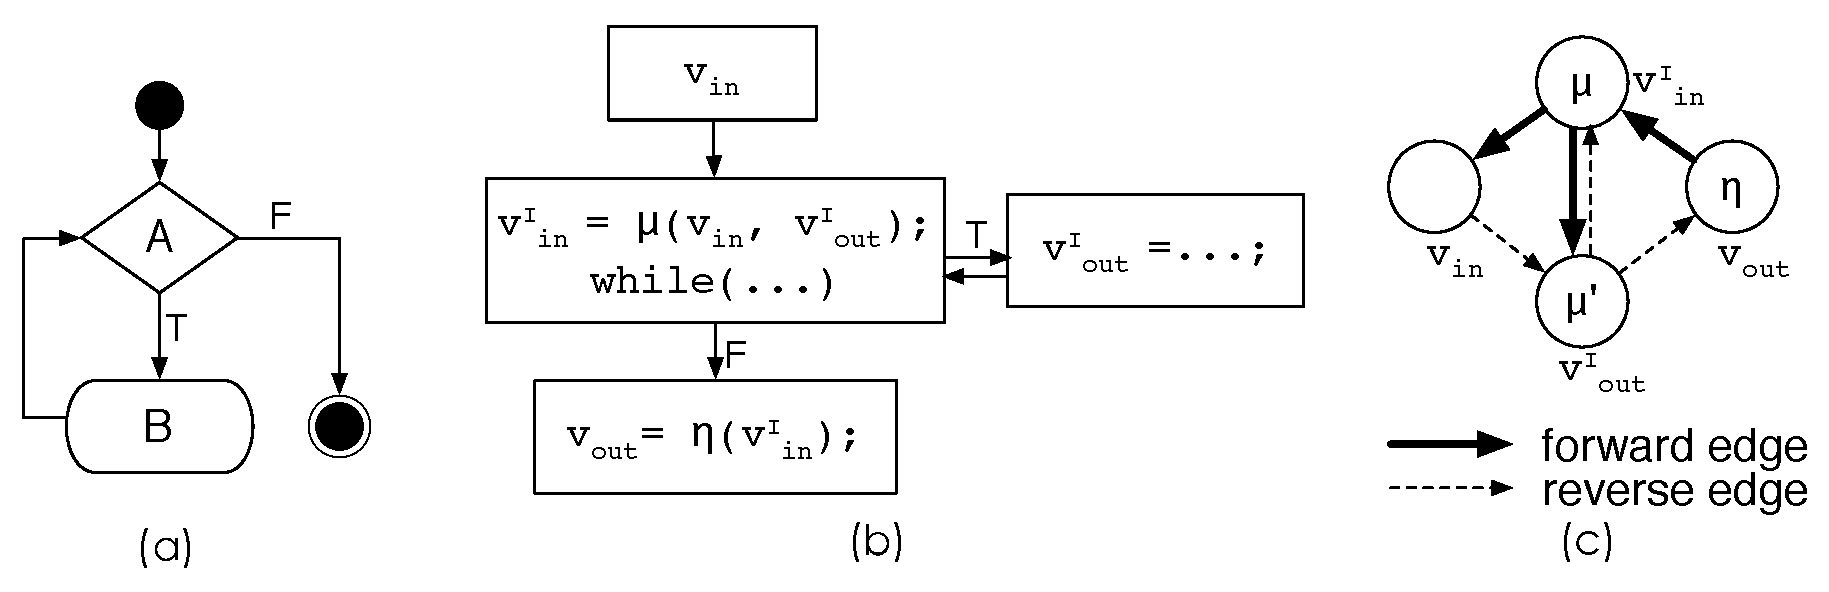
\includegraphics[width=400pt]{figures2/simpleLoop.pdf}}
\caption{(a) The diagram of a while loop. (b) The CFG in loop-closed SSA form for a variable $v$ modified in the loop. (c) Forward and reverse edges.}
\label{fig:loop_example}
\end{figure}

\subsection{Dealing with while loops}
\label{sec:while-loops}

%Let's first look at a simple while loop example. 
We first consider a while loop with the diagram shown in Figure~\ref{fig:loop_example}(a).
We further assume that $A$ has no side-effects %
%
%\footnote{A more loose condition is that a definition can exist in $A$ as long as this definition is only ``live'' in the loop, i.e., is not used outside of the loop.}
%
and that there are no escapes from $B$.
Thus, the loop only exits from its entry.  

Given such a while loop, we transform it into the \emph{loop-closed SSA form}~\cite{Pop2009}, illustrated in Figure~\ref{fig:loop_example}(b).
Loop-closed SSA differs from conventional loop-free SSA as follows.
In conventional SSA, a special marker called a \emph{$\phi$ function} is placed in the CFG at the first program point where two distinct versions (definitions) of a variable, computed along different program paths, meet.
%
In loop-closed SSA, if a value is defined inside of a loop and used outside of it, we place a special single entry $\phi$ function at the \emph{exit} of the loop.
To distinguish this type of loop-specific $\phi$ function from a conventional $\phi$ function as used in loop-free programs, we denote the loop-specific form by the term $\eta$ function, by convention~\cite{RobertA.Ballance1990}.
Additionally, suppose a definition of a variable from outside the loop and a definition coming from a back-edge of the loop meet at a program point.
Again, we create a $\phi$ function marker here, and to distinguish it, we refer to it as a $\mu$ function.

To see how these markers work, consider a variable $v$ modified by a while loop;
we now describe the corresponding loop-closed SSA form, which Figure~\ref{fig:loop_example}(b) illustrates.
Let \vinit denote the input value of $v$ before the loop executes, and \vfinal the output value of $v$ after the loop executes.
Next, let the input to the loop \emph{body} be \vmu and the output \viter.
(The superscript $I$ is intended to remind the reader that these are values associated with an \emph{iteration} of the loop, as opposed to the values before and after the loop.)
Then, \vmu is defined by a $\mu$ function as \mufunc, and \vfinal is defined by a $\eta$ function as \etafunc.
That is, \mufunc indicates the program point at which $v$ has either the initial value before the loop executes or the value produced by some iteration of the loop;
and \etafunc indicates the program point at which $v$ has the final value once the loop completes.
%We will consider the problem how to generate a forward loop 
%Now let's construct the VSG for generating the forward and reverse loops.

From this loop-closed SSA form, we wish to build a VSG that will express equality relations among the four SSA values, \vinit, \vfinal, \vmu, and \viter.
This VSG result is shown in Figure~\ref{fig:loop_example}(c).
Recall that nodes in the VSG represent values, and edges the equality relations.
%
%The loop-collapsed \pVSG comes from the left-hand column of nodes from Figure~\ref{fig:loop_example}(b) and is shown in Figure~\ref{fig:loop_example}(c) as the upper three nodes and upper two solid edges.
%The loop body \lVSG comes from the right-hand node of Figure~\ref{fig:loop_example}(b) and results in the bottom node of Figure~\ref{fig:loop_example}(c).
%
%Now we consider the problem how to retrieve \vfinal or \vinit from \lVSG.
%If we could do that, a loop will be generated in the reverse program producing \vfinal or \vinit.
%
There are four value nodes.
The nodes \vinit and \vfinal are part of the loop-collapsed \pVSG, and \vmu and \viter belong to the loop body's \lVSG.
The $\mu$ and $\eta$ functions indicate how to connect \pVSG and \lVSG.
In particular, the three solid bold edges are associated with the dependences induced by executing the loop in the forward direction;
we call these the \emph{forward edges}, and a $\mu$ node is incident to all three.
The presence of these edges make it possible to obtain \vfinal by some path passing through \lVSG, and simultaneously indicate that a loop is present for subsequent code generation.
Similarly, the three dashed edges are \emph{reverse edges} associated with dependences induced in the reverse direction.
These edges make it possible to obtain \vinit by some path through \lVSG.
Note that the reverse edges form a symmetry to the forward edges.
From this symmetry, we define the node incident to all three reverse edges as a $\mu'$ node.
Later we will show how the search traverses these edges.

Having built the CFG, the next step is to search it, producing the RG result.
Recall that we are given a set of target nodes whose values we wish to eventually compute from a starting set of available nodes.
We search for a path from available nodes to target nodes; the subgraph representing paths is the RG, which is not necessarily unique.
Our algorithm is similar to the one we have described previously~\cite{Hou2012}, but for loops we need three additional search rules:

\begin{itemize}
\item During a search for a value, once a forward/reverse edge is selected, all edges in the other category cannot be chosen. This is because either a forward or a reverse loop will be built to retrieve the value.

%To build a forward loop, if the search reaches a $\mu$ node, it forks by advancing through the two outgoing forward edges; to build a reverse loop, if the search reaches a $\mu'$ node, it forks by advancing through the two outgoing reverse edges. 
\item When the search reaches a $\mu$ or $\mu'$ node, it will be split into two sub-searches, in \pVSG and \lVSG, respectively, through the two outgoing forward or reverse edges.
For example, in Figure~\ref{fig:loop_example}(c), if the search reaches \vmu, the algorithm begins two sub-searches beginning with \vinit and \viter.

%As we discussed above, if at compile time we can determine that the loop body will certainly be traversed at runtime, the search does not fork but continues toward \viter or \vmu.
\item During the search, the algorithm may form a directed cycle only in \lVSG; furthermore, such a cycle must contain a forward or reverse edge between a $\mu$ and $\mu'$ node. 
Once a cycle is formed, the search in \lVSG is complete.
%will not move further from the current node just like when an available node is reached.
\end{itemize}

\noindent
We build a while loop as either a forward or a reverse loop. 
Synthesizing such a while loop consists of synthesizing its body and predicate.


\subsubsection{Building the loop body.}

The loop body in the reverse program is generated from the search result in \lVSG.
For each variable we remove the edge between the $\mu$ and $\mu'$ nodes and hence remove the cycles, so that we can generate the loop body using our prior code generation algorithm.

%there is no cycles any more. 
%As a result, this subgraph of the RG used to build the loop body connects each \viter or \vmu (for forward or reverse loop) to the $\mu$/$\mu'$ node or value nodes not defined in the loop. The code is generated in the same method as in \cite{Hou2012}. 
%Since recording control flows in a loop may be expensive, we will use the method mentioned in the previous section which retrieves each value in the predicate. If this method does not work, we have to record the control flows for all iterations using a bit vector. It is possible that the cost to store control flows offsets the benefit to retrieve a value from a loop which may not need a state saving. In this case, we can turn to the method in \cite{Hou2012} which is a better choice.

\begin{comment}

\begin{figure}%[htb]
\center{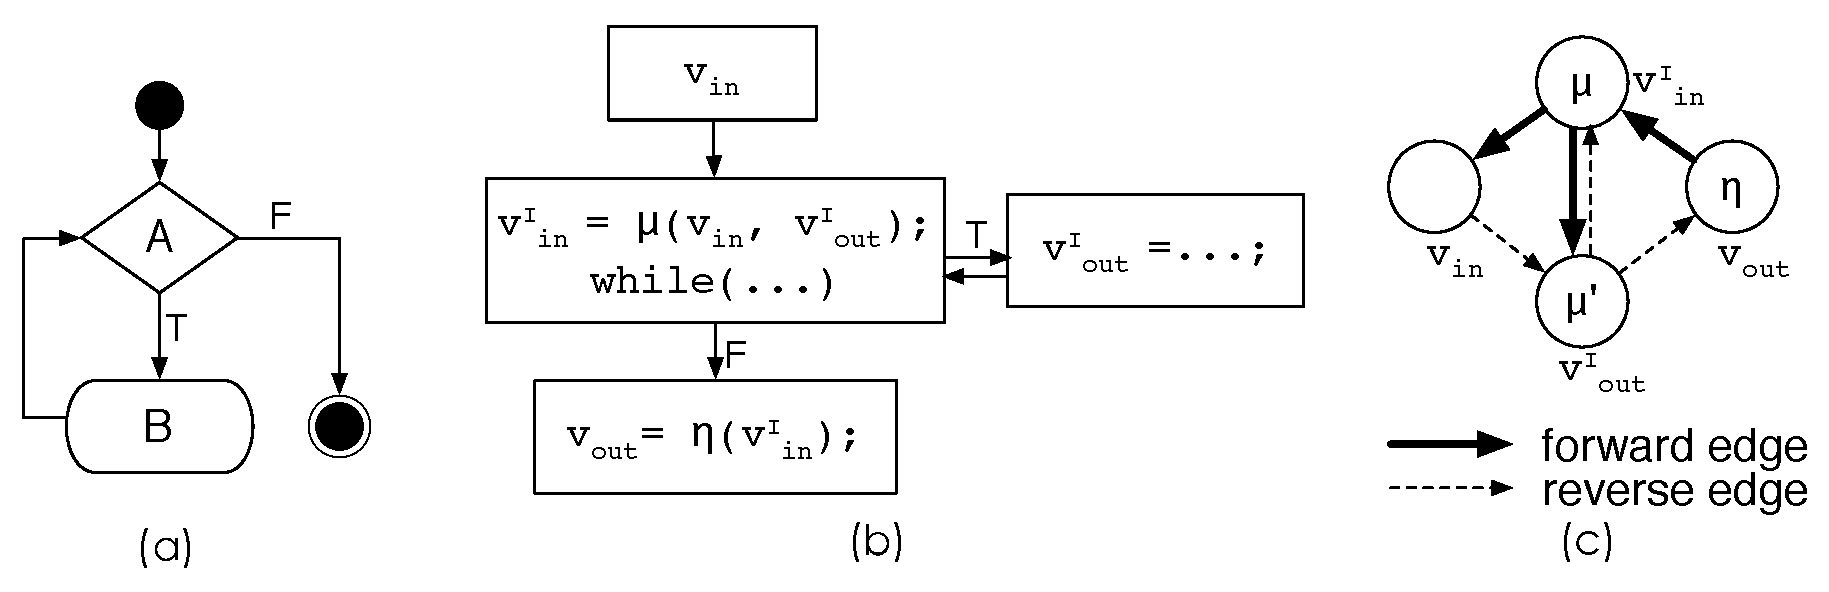
\includegraphics[width=300pt]{figures2/loopExample.pdf}}
\caption{(a) The VSG for our example. (b) The RG for retrieving $a_3$ and $i_3$. (c) The RG for retrieving $a_0$.}
\label{fig:loopExample}
\end{figure}

\end{comment}



%Our search begins from the node $a_0$ in Figure \ref{fig:loop_vsg}(a). Once we go from $a_0$ to $a_1$ into the loop block\footnote{\TODO{need we define this term?}}, we are selecting to build a reverse loop, and we will add some restrictions during the search: all edges belonging to the forward execution should not be taken. 

%In [], we forbid any circle during the search for each CFG path, however, since we are building another loop, we permit the circle to appear in the search result, with one requirement: each circle should contain the edge between $v_{\mu}$ and $v_{iter}$.



%The loop body generated from Figure \ref{fig:loop_vsg}(b) is \texttt{\{ i = i + 1; a = a + i;  \}}, and the loop body generated from Figure \ref{fig:loop_vsg}(c) is \texttt{\{ a = a - i;  i = i - 1; \}}.


\subsubsection{Building the loop predicate.}

To guarantee that the generated loop has the same iterations at runtime as the original loop, we need to build a proper loop predicate. 
We propose three approaches to building a correct loop predicate. 
To illustrate those approaches, we temporarily introduce the following loop example. We assume that the omitted statements  modify neither \texttt{A[]} nor \texttt{i}.

\begin{lstlisting}
i = 0;
while (A[i] > 0) {
    /* ... */
    i = i + 2;
}
\end{lstlisting}



%The first two approaches are preferred since they may not need any instrumentation to the original loop, but cannot be always applied, and the third one needs an instrumentation to the forward program and is always working. 

\begin{itemize}
\setlength{\itemsep}{5pt}%

\item \textbf{Approach 1:} Building the same loop predicate as that in the original loop. 
To build this predicate, we need to retrieve each value in the predicate.
%, we need to retrieve its input value of the loop before the loop, and if it is updated in the loop, we also need to retrieve its input value of the loop body in the loop. 
A new search is needed to acquire those values, and the search result will be combined into the RG generated above.
For the example above, we can build a loop below that has the same number of iterations as the original one. The omitted statements will be substituted by the loop body built above.


\begin{lstlisting}
i = 0;
while (A[i] > 0) {
    /* ... */
    i = i + 2;
}
\end{lstlisting}



%In the second case, we  
%$a$ for example, if it is not modified in the loop, we need to retrieve the value of $a$ before building the while condition; if it is defined by a $\mu$ function as $a_{in}^I = \mu (a_{in}, a_{out}^I)$, both $a_{in}$ and $a_{out}^I$ should be retrieved. 
%Figure \ref{fig:rvsLoops}(a) shows the resulted loop built from this approach.
%This is done by starting another search beginning with $a_{in}^I $. Note that we also updated the loop body to include the statement that defines $a_{out}^I$.


\item \textbf{Approach 2:} Building the loop predicate from a variable updated in the loop. Given a variable $v$ and its four definitions: \vinit, \vmu, \viter, and \vfinal, if \vmu$\ne$\vfinal in each iteration except the last definition of \vmu (which is actually \vfinal), and if we can retrieve \vinit and \vfinal before the loop (hence we cannot retrieve them through the loop), and \viter in the loop, we can use them to build a while loop as:
$$
u := v_{in}; \;\\
while (u \ne v_{out}) \;  \{\; 
/* \; update \; u \; */ \; 
\}
$$

Similarly, if \viter$\ne$\vinit  in each iteration, and  \vinit and \vfinal can be retrieved before the loop, and \vmu can be retrieved in the loop, we can use them to build a while loop as: 
$$
u := v_{out}; \; while (u \ne v_{in}) \;  \{\; /* \; update \; u \; */ \; \}
$$

In general, it is difficult to detect all variables satisfying the properties above.
However, there are some special cases.
One case is that of \emph{monotonic variables}~\cite{Wolfe1992}, which are monotonically strictly increasing or decreasing in each iteration.
Another is that of induction variables, which are special monotonic variables that are relatively easier to recognize. In the above example, \texttt{i} is an induction variable. Assume its final value after the loop is \texttt{i1} that is known, and then we can build the following loop with the predicate using \texttt{i}.



\begin{lstlisting}
i = 0;
while (i != i1) {
    /* ... */
    i = i + 2;
}
\end{lstlisting}


%Indeed, the first approach above is a special case of this one if we define another Boolean variable $c$ as $a < b$, where $c$ satisfies the condition above.
 %Instead, we only detect variables which are updated during iterations monotonically. Note that induction variables fall into this category which are easier to detect.
%loop variant. A loop variant is a variable whose value is updated in each iteration monotonically\footnote{This is too strict: \TODO{distinct values are also OK.}} and the while condition is a comparison between the loop variant and another value. Assume the loop variant is $i$ with initial value $i_{init}$ and final value $i_{final}$, and in all iterations, $i$ is increased or decreased monotonically. If we can retrieve $i_{init}$ and $i_{final}$, plus $i_{\mu}$ or $i_{iter}$ in each iteration, we can use this variable to build the while condition for the forward or reverse loop. Specifically, a forward loop \TODO{Note that it does not make sense to classify a loop as a forward or reverse one, since they may appear in the same loop} is built like:
%To build the while condition, we first detect all loop variants in the loop (\TODO{how?}). For each loop variant $i$, we have to retrieve both $i_{init}$ and $i_{final}$, and depending on whether the generated loop is forward or reverse, we have also to retrieve either $i_{\mu}$ or $i_{iter}$. 
%Because at the beginning of the loop, we should already have $i_{init}$ and $i_{final}$, we cannot retrieve them through the loop. This means the search should not reach the loop nodes from them. The search for $i_{\mu}$ or $i_{iter}$ follows two forward or reverse edges as described above. 
%In case that there are several candidates satisfying the requirement above, for each variable, we calculate the cost to retrieve all dependent values and choose one with the least cost to build the loop predicate. 
%In our example, both $a$ and $i$ are monotonic variables, but  $a$'s initial value is unknown (which is what we are retrieving!). In contrast, $i$'s initial and final value are 0 and $N$, and $i$ can be updated either by a forward loop beginning with its initial value, or a reverse loop beginning with its final value. Figure \ref{fig:rvsLoops}(b) and (c) shows those two results. Note that in Figure \ref{fig:rvsLoops}(c) the code retrieving $i$ in the loop body is shared with the loop body generated before \TODO{!}.


\begin{comment}
\begin{figure}%[htb]
\center{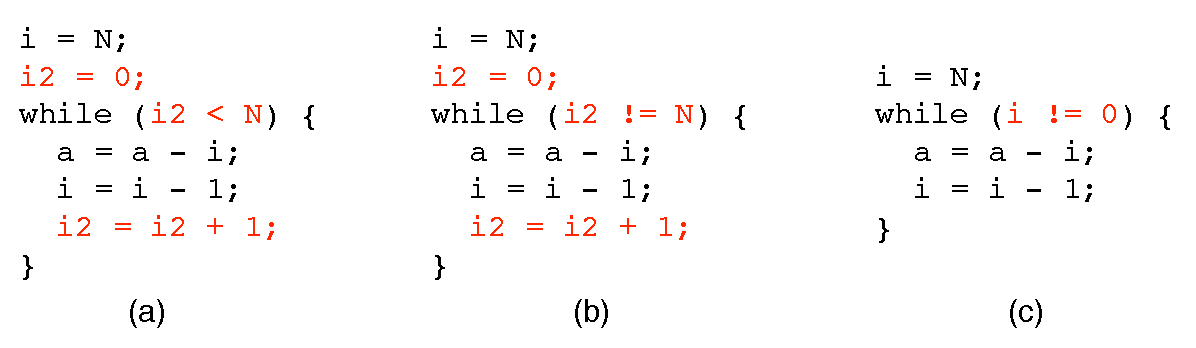
\includegraphics[width=300pt]{figures2/reverseLoops.pdf}}
\caption{Three results.}
\label{fig:rvsLoops}
\end{figure}
\end{comment}

%However, it is possible that we cannot find such a loop variant. (Although every loop that terminates has a variant). 
%The reason is that the loop variant we are looking for is somehow special, but it is possible \TODO{see wiki: Transfinite induction}. 
\item \textbf{Approach 3:} Instrumenting the original loop with a counter counting the number of iterations. The counter has the initial value zero and is incremented by one on each back edge of the loop.
The final value of the counter is stored in the forward program and restored in the reverse program as the maximum value of another loop counter.
This approach generally works if either of the above two approaches fail.
However, it requires instrumentation (the counter), and therefore forces generation of a forward program. Below we show the instrumented loop in the forward program (first) and the generated loop in the reverse program (second) for the above example.

\begin{lstlisting}
i = 0;
count = 0;
while (A[i] > 0) {
    /* ... */
    i = i + 2;
    count = count + 1;
}
\end{lstlisting}


\begin{lstlisting}
while (count > 0) {
    /* ... */
    count = count - 1;
}
\end{lstlisting}


\end{itemize}

We prioritize these approaches as follows.
Applicability and state-saving cost are our main criteria.
We prefer Approach 1 and 2 over 3.
When either 1 or 2 apply, if no state-saving is required, we apply them.
Otherwise, we try Approach 3 and choose the overall approach with the least cost.

\vspace{3mm}

\begin{figure}%[htb]
\center{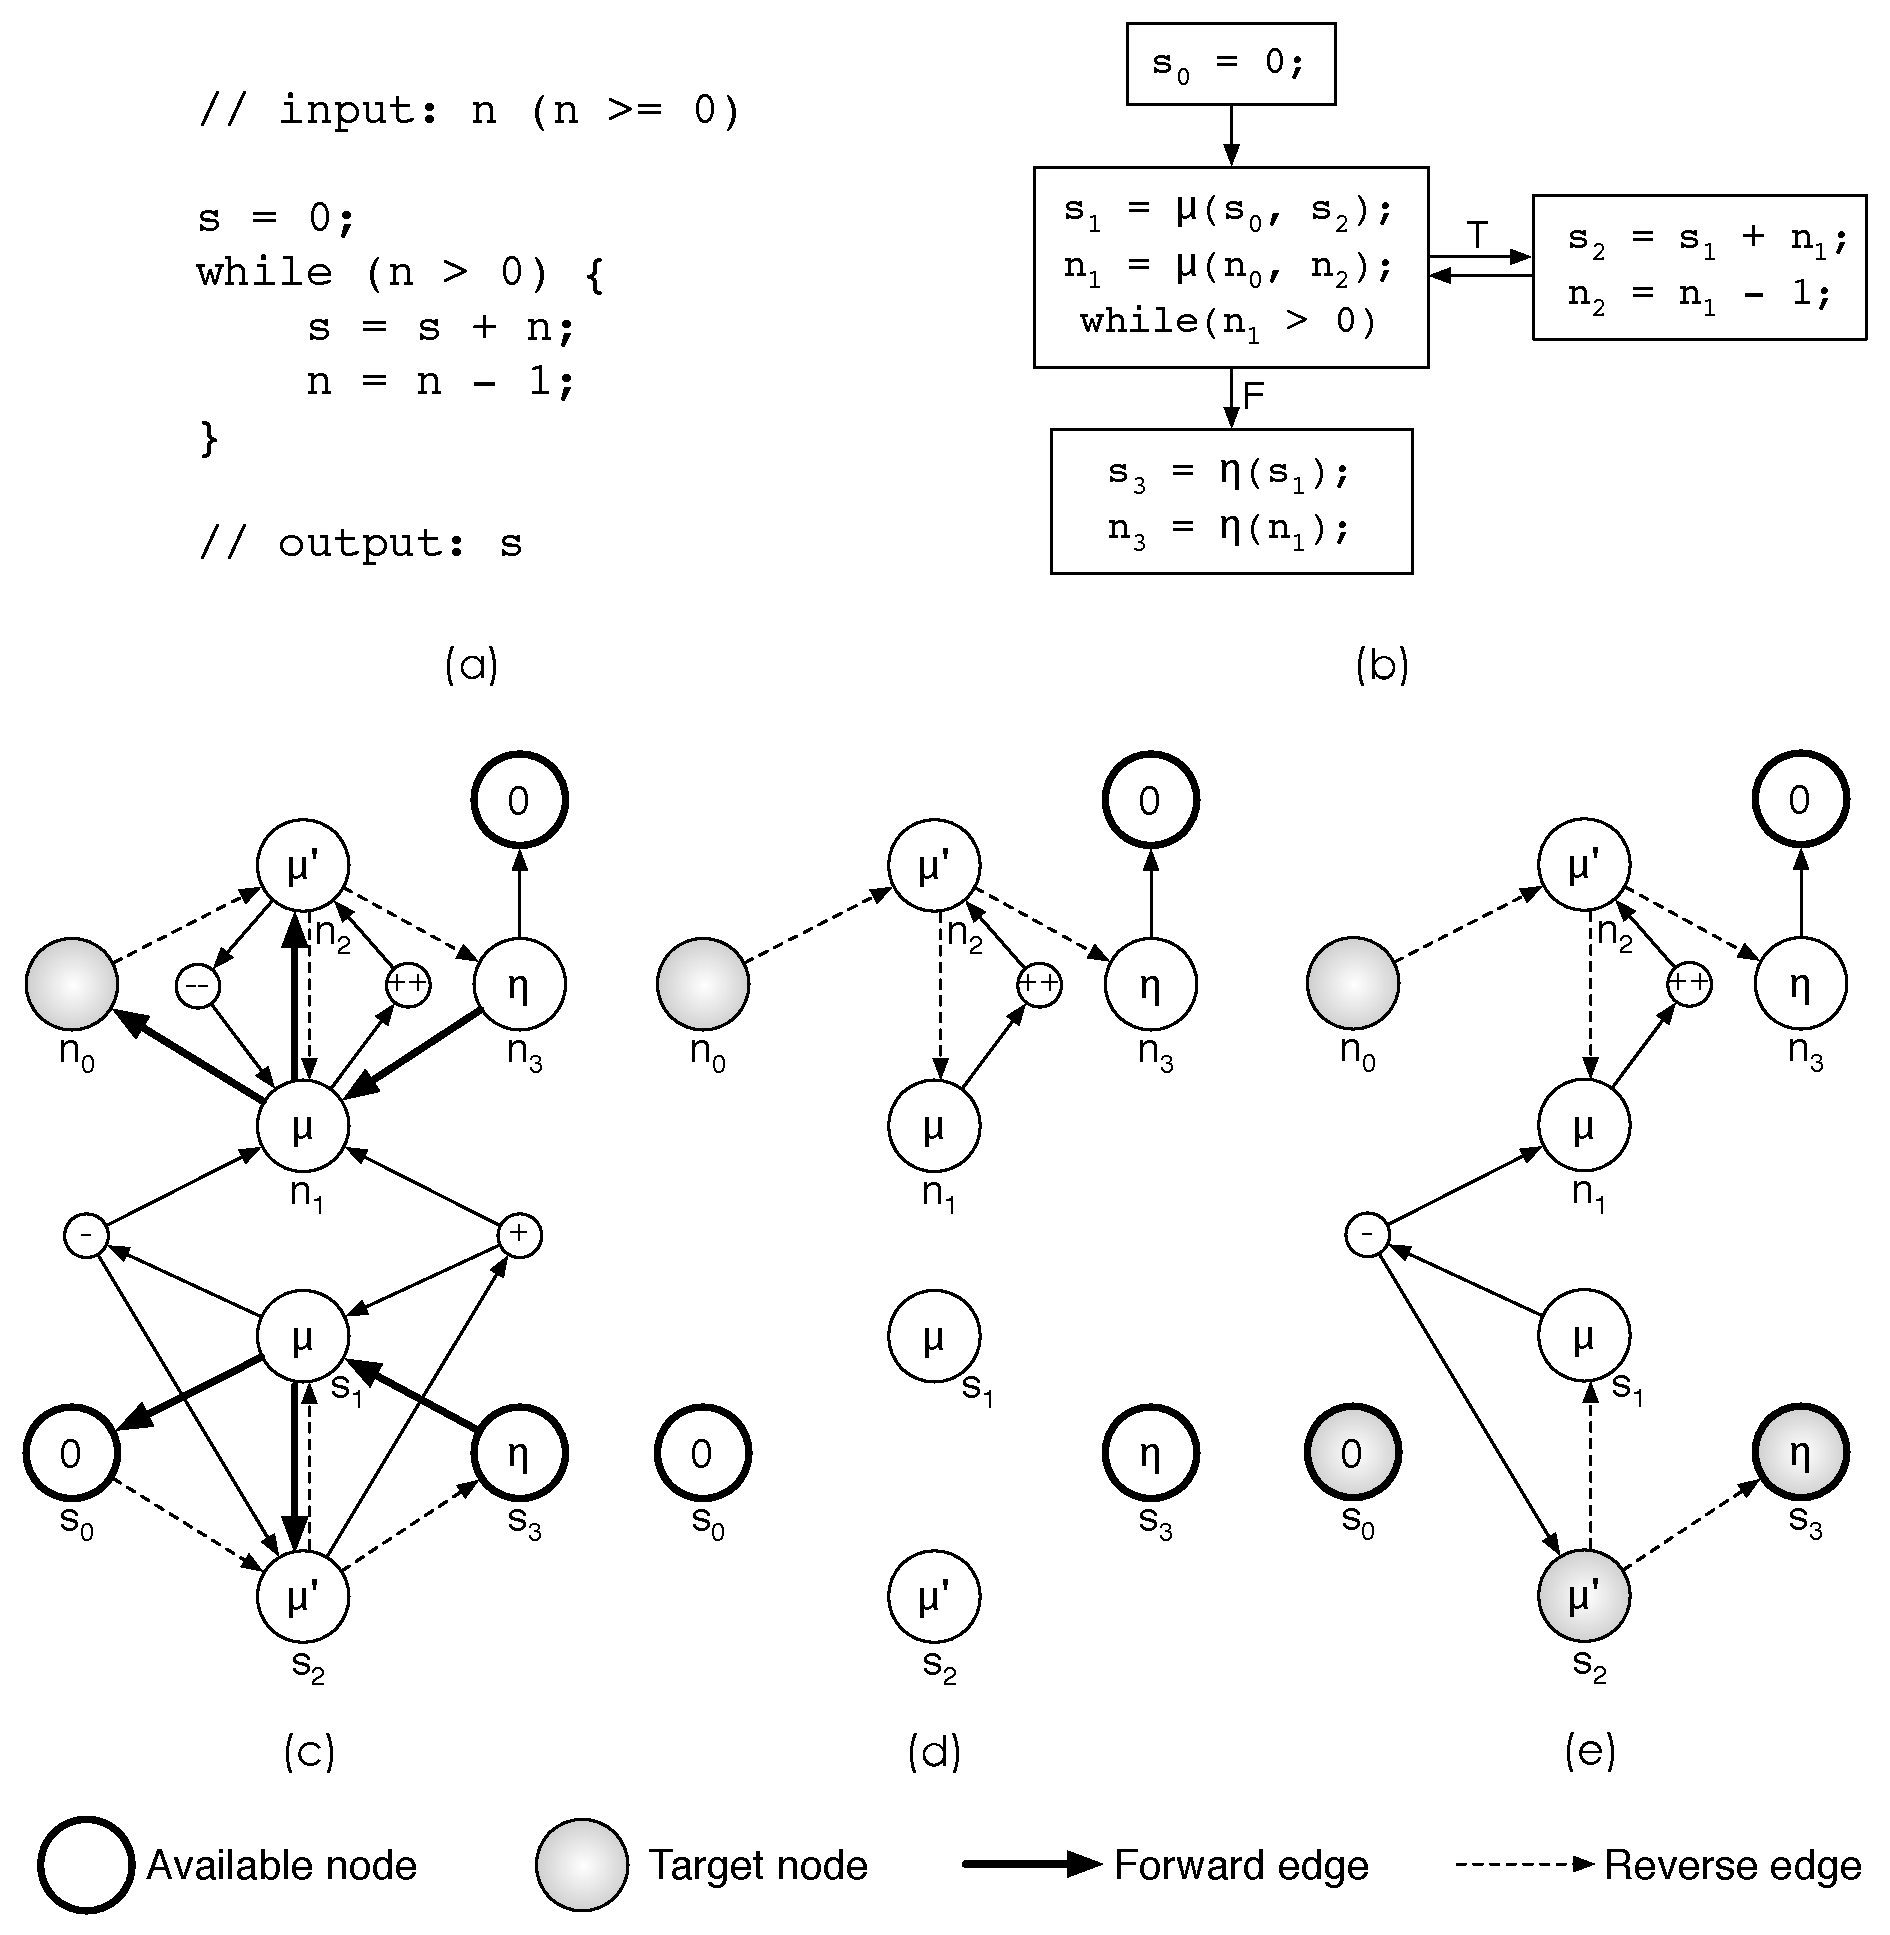
\includegraphics[width=400pt]{figures2/loopVSG.pdf}}
\caption{(a) The program of our example. (b) The CFG in loop-closed SSA form. (c) The VSG.  (d) The RG for retrieving $n_3$. (e) The RG for retrieving $n_0$ and $s_2$.}
\label{fig:loop_vsg}
\end{figure}

As an example, suppose we apply this algorithm to the loop in Figure~\ref{fig:loop_vsg}(a).
Figure \ref{fig:loop_vsg}(b) shows its CFG in loop-closed SSA.
The input is $n_0$ and the output $s_3$.
Our goal is to generate a reverse program that takes $s_3$ as input and produces $n_0$.
We build the VSG shown in Figure~\ref{fig:loop_vsg}(c), with forward and reverse edges shown as bold and dashed edges, respectively.
Note that the equality between $n_3$ and 0 is acquired from solving constraints, a standard compiler technique.%
%
\footnote{For clarify, we remove the equality $n_1=s_2-s_1$, as this relation will not be used during the search.}
%
The search result for value $n_0$ is shown in Figure \ref{fig:loop_vsg}(d), from which we can build the loop body as \texttt{\{ n = n + 1;  \}}.

Next, we build the loop predicate.
In our example, because we wish to retrieve the initial value of $n$, we cannot use it to build the loop predicate.
We can discover that $s$ is a monotonic variable, and that both the initial and final values of $s$, which are 0 and $s_3$, respectively, are available.
To get $s_2$, we search its value on the VSG and the search result is shown in Figure \ref{fig:loop_vsg}(e). 
As a result, we build the loop predicate from $s$ and the reverse program is generated as below.


\begin{lstlisting}
while (s != 0) {
    n = n + 1;
    s = s - n;
}
\end{lstlisting}


Above we have built a reverse loop in the reverse program, but it is also possible that the reverse program contains a forward loop. 
For instance, if we change our example into the program shown  below:


\begin{lstlisting}
s = 0;
i = 0;
while (i < n) {
    i = i + 1;
    s = s + i;
}
\end{lstlisting}


Without modifying its semantic, its inverse will contain a forward loop which is shown below:

\begin{lstlisting}
s2 = 0;
i = 0;
while (s2 != s) {
    i = i + 1;
    s2 = s2 + i;
}
n = i;
\end{lstlisting}

 This is because the input of the new program $n_0$ is equal to $i$'s final value, which is the output of the loop. 

%\subsubsection{Other single-exit loops}
%The while loop we discussed above is just one kind of the single-exit loops. %Do-while loop is another single-exit loop. 
%For other single-exit loops, we can transform them into while loops, and we can also utilize the similar technique as above to handle them. However, as we will see later, the transformation described below can handle those cases including loops with several exits. 

\subsection{Dealing with loops other than while loops}
\label{sec:other-loops}

In practice, the vast majority of loops have a single entry, which are called \emph{natural loops}~\cite{Muchnick}. 
Loops with more than one entry are quite rare and can in fact be transformed into natural loops~\cite{Muchnick}. 
However, it is quite common that a loop has several exits. 
For example, in C/C++ we may exit a loop early through \texttt{break}, \texttt{return}, or \texttt{goto} statements.
Nevertheless, given a non-while natural loop, we can transform it to separate the last iteration from the loop;
then, the remaining iterations form a new while loop, and the last iteration will not belong to the loop and hence can considered with the control flows outside of the loop. 
We then process the new while loop as previously described.
Note that this ``transformation'' is only applied to the CFG during the analysis, and not to the original program.
As such, in the forward program \Forward the last iteration and other iterations of each loop continue to share the same code.


Figure~\ref{fig:loop}(a) shows a loop in a CFG, with a header (node 1) and two back edges (4$\to$1 and 5$\to$1). 
There are two different exits from this loop, which are nodes 6 and 7.
%An exit edge of a loop is an edge connecting a loop node to an exit. 
%1$\to$6 and 3$\to$7 are two exit edges.
Figure~\ref{fig:loop}(b) shows the CFG of the transformed loop.
This transformation is performed as follows.

In a natural loop, only the last iteration takes the exit, and any other iteration goes back to the loop header.
Therefore, if the last iteration is peeled off from the loop, this loop will turn into a while loop. 
%Suppose we can predicate the number of iterations (the number of back edges being traversed) before a loop is taken, which is although impossible for most loops. Let \texttt{k}  be a virtual variable whose value is the number of the back edges being taken at runtime, 
To implement this transformation, we create a new branch node with an unknown predicate that returns $true$ if the next iteration is not the last one and $false$ otherwise.
Note that we will not build this predicate in the forward program. 
The new branch node turns over all in-edges of the loop header. 
%Note that  \texttt{k}'s initial value usually cannot be determined at compile time, but we are not actually doing this transformation to the original function and hence it won't bring any problem here. 
Its $true$ labeled out-edge will point to the loop header of a copy of the loop (node $1'$) with back edges but without exit edges, and all back edges are redirected to this new branch node making it a new loop header. 
Note that after removing exit edges it is possible that a previous branch node becomes a non-branch node (node $3'$, for example), which is fine because the removed branch edge will not be taken. Then, we can remove the (side effect free) predicates from those nodes. The edge labeled with $false$ from the new branch node will point to the original loop header (node 1) and all back edges in the original loop are removed, since the last iteration won't take the back edge. The nodes from which the exit of the program is not reachable due to the back edge removal are removed (node 4 and 5, for example). Again the predicate is removed from a node once it is not a branch node anymore (node 2 and 3).
%Fig \ref{fig:loop}(b) shows the transformed flow graph where the node 0 is the new branch node and loop header. Note that the node 4 and 5 are removed since they are not reachable anymore.
 %At runtime, the true edge must be traversed and the false edge may not. 
%The true edge postdominates the false edge, but the latter does not dominate the former. 

\begin{figure}%[htb]
\center{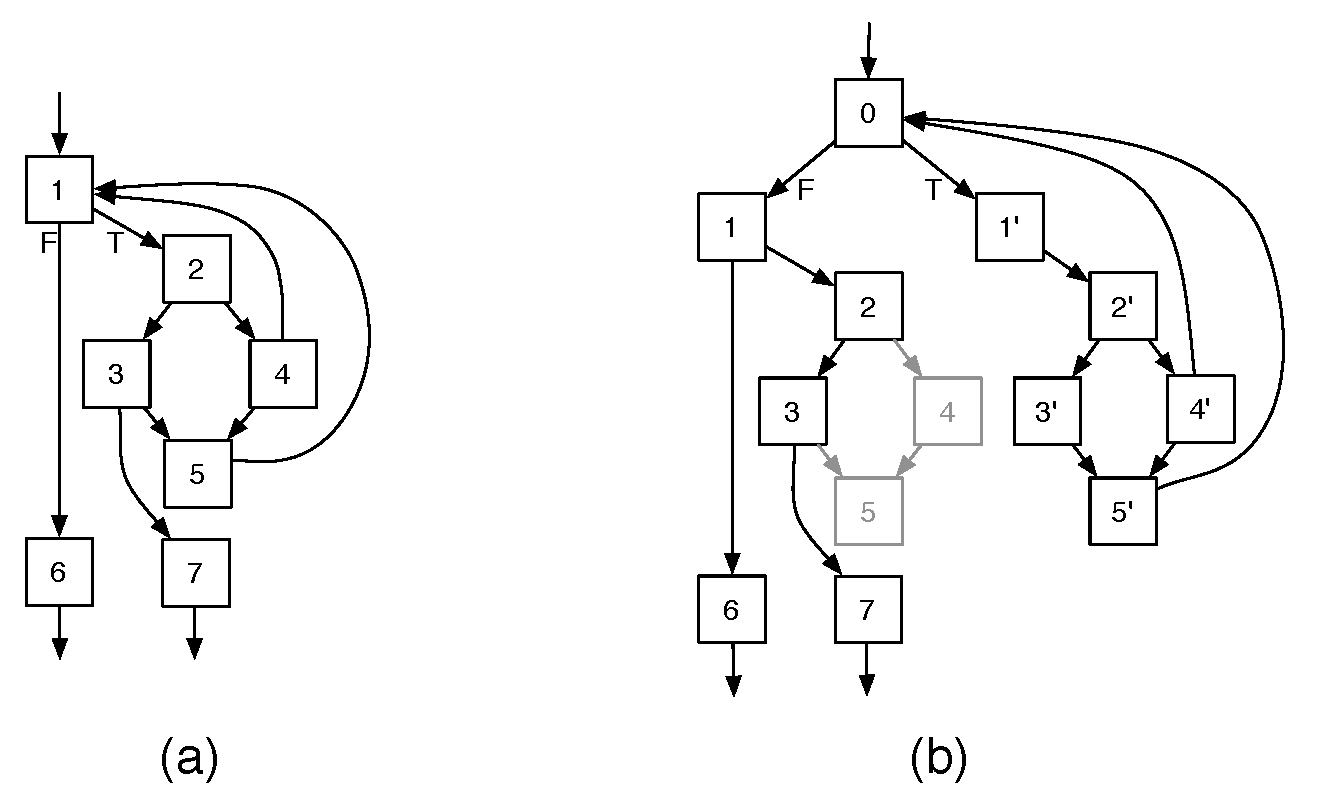
\includegraphics[width=350pt]{figures2/Loop.pdf}}
\caption{(a) A loop in CFG with two back edges and two exits. (b) The CFG of the transformed loop.}
\label{fig:loop}
\end{figure}

After the transformation, all loops in the program become while loops and our method applies.
Since the new generated loop predicate  is unknown, to build the loop predicate  in the reverse program, we cannot use the first approach proposed above any more. %Therefore, it is preferred that a loop be transformed into a while loop normally, not in the above method. For example, a do-while loop can be easily converted into a while loop.

Because those two newly created branch bodies share the same code in the forward program,  any instrumentation will also be shared between them. 
For example, if a value defined in the false body above needs a state saving, in the forward program we can only perform the state saving in the loop, which results in saving a value many times and then larger time overhead. 
For this reason, we could forbid state savings on any variable in the false body.
Properly defining the cost of this operation may help to get the better search result. 
%On the other hand, if a state saving is made from reversing the loop hammock, at the exit of the loop, any side effect should be taken care. For example, if a stack is used to store variables, the pop operations may be needed at the exits.




%============================================================
%============================================================


\chapter{Synthesis for programs with arrays}
\label{chapter:arrays-loop-free}

In this chapter, we extend the previous method to handling arrays in both loop-free programs and those with loops.
We will still use the same framework. 
That is, we will build a VSG for the program with arrays, then perform a search on it to build a RG.
Then we translate the RG into the source code.
%There are two motivations for us to handle arrays: in OPDES, storing an array is very expensive. We need to improve the performance by using as less state savings as possible on arrays. If we can avoid performing state saving on an array that is modified in a loop and can be retrieved by another loop in the reverse program, the performance will be improved; 
%we also consider to generate the inverse for injective programs, such as lossless compression and encryption,  when state saving is not allowed (because the program is already injective or reversible, it is not necessary to generate a forward program). 
%Arrays are a particularly important case: naively saving the entire array too frequently will be very expensive in space and time. Our method permits saving of just the elements that have changed, and better yet, can often use cheaper computation in place of state saving.
To build the VSG for arrays, we apply a modified Array SSA based on \cite{rus2006scalable}, and define several special VSG nodes for arrays. 
To represent the equality between two arrays, we employ the array subregion as the constraint. 
During the search those subregions will be calculated to guarantee that all array elements will be retrieved. We also develop a demand-driven method to retrieve array elements from a loop. 

%============================================================
\section{Handling loop-free programs with arrays}
\label{sec:array-loop-free}
\newcommand{\arraylen}{\ensuremath{a.length}\xspace}
\newcommand{\EquivRange}[3]{\ensuremath{(#1\equiv#2)@#3}\xspace}

We first consider how to extend the VSG and RG machinery to handle arrays in loop-free programs.
(We treat loops in Section~\ref{sec:array-loops}.)
%, and propose a method to deal with more challenging programs with loops in the next section.
%In this section, we first introduce the Array SSA, then describe how we make use of it and build array nodes and edges in the VSG. 
%Then we still divide the programs with arrays into two categories: programs without and with loops. 
%In this chapter we will use an Array SSA proposed in [] in which concrete array regions are employed.
%Based on this Array SSA, we could build the VSG with special array nodes inside.
%By modifying the searching rules on the VSG, we will see that we could handle programs with arrays using the same framework as before. 
The key idea behind our method is explicit representation of array subregions (subsets of array elements) combined with a modified form of Array SSA~\cite{rus2006scalable}.

\subsection{Array subregion representations and operations}

%Unless explicitly indicated, when we retrieve an array, we are retrieving all elements of it. 
Given an array $a$ with length \arraylen, all elements can be represented by their indices as an interval $[0,\arraylen)$.
We denote this index set, $[0,\arraylen)$, as the \emph{universal set}, $\mathcal{U}(a)$.
A (strict) subregion of $a$ is a (strict) integer subset of the universal set.

Among all possible subregions of an array, notable cases we will consider include:
%
\begin{itemize}
\item The subregion containing a single index $i$, denoted $\{i\}$, where $i$ is a constant or an SSA name.
%\footnote{Note that an SSA name normally has a version. But for clarity we ignore this version when it is unnecessary to show it.}. 
\item The set of all indices other than $i$, or $\overline{\{i\}} = \mathcal{U}(a)-\{i\}$.

\item The triplet $[p:s:q]$ is the set of all indices starting from $p$ up to (and possibly including) $q$ with stride $s$. We use the shorthand $[p:q]$ when $s=1$.
\end{itemize}

We need index set operations so that our analysis algorithm can conclude whether or not we have restored all elements of the array on all paths.
However, our analysis, being symbolic at compile-time, will also need to be conservative.
%All set operations can be performed on array subregions. Actually, later during the search we will use those operations on array subregions and inspect the results to guarantee that all array elements in a specific subregion are retrieved. 
%However, because of symbols in subregions, we could not get the result of every set operation if some necessary informations are missing.
For example, given an intersection $\{i\} \cap \{j\}$, the result of it could be  $\{i\}$ or $\emptyset$, depending on whether $i=j$ or $i\ne j$, which may be indeterminate at compile-time.
As such, key operations we will use are:
%, which, however, possibly could not be determined at compile time.
%From the operations and the results shown below, we can conclude that checking the equality and inequality between two symbols at compile time is essential to get the results.

$$
\{i\}\cap {\{j\}} = \left\{ \begin{array}{ccl}  \{i\} & \mbox{if }  i = j \\ \emptyset & \mbox{if }  i \ne j  \end{array}\right.
$$
$$
\{i\}\cap \overline{\{j\}} = \left\{ \begin{array}{cc}  \{i\} & \mbox{if }  i \ne j \\ \emptyset & \mbox{if }  i = j \end{array}\right. 
$$
$$
\{i\}\cup {\{j\}} = \left\{ \begin{array}{cc}  \{i\} & \mbox{if } i = j \\ \{i\}\cup {\{j\}}  & \mbox{if }  i \ne j \end{array}\right. 
$$
$$
\{i\}\cup \overline{\{j\}} = \left\{ \begin{array}{cc}  \mathcal{U} & \mbox{if } i = j \\ \overline{\{j\}} & \mbox{if }  i \ne j \end{array}\right.
$$
$$
\{i\}\cap [p:q] = \left\{ \begin{array}{cc}  [p:q] & \mbox{if } i \ge p \mbox{ and } i\le q \\ {\emptyset} & \mbox{if } i < p \mbox{ or } i> q \end{array}\right.
$$

%But at compile time if we can determine if $i=j$  or $i\ne j$, we cat get the result of this intersection as $\{i\}$ or $\emptyset$.
%Or else, we will leave the operation there. 
%In order to build a more accurate RG, we need to simplify an expression with set operations.

Because the VSG reveals equalities between values, we can use it to check if $i=j$ by starting a path search from $i$ to $j$. 
To check inequality, we can use the previously proposed \emph{inequality graph} ~\cite{ABCD}.
In this representation, each node is a constant or an SSA name;
each directed edge $x \xrightarrow{c} y$ represents $x-y\le c$. 
The inequalities are obtained from, for instance, branch predicates like $\texttt{if}(x>y)$ and assignments like $x = y + c$, where $c$ is a constant. 
From the inequality graph, checking whether $x \ne y$ is equal to checking if $x-y\le -1$ or $y-x\le -1$.
%Note in our application we don't care if $a>b$ or $a<b$.
%Therefore, we can make use of more informations like the predicate $if(a\ne b)$ and $if(a=b)$ (where $a\ne b$ in the false body).

As our analysis manipulates and simplifies set operations, we may need to normalize the operations according to the set operation laws, including identity laws, domination laws, idempotentency, commutativity, associativity, distributivity, among others.
%In addition, since an array subregion may contain SSA names. 
%The knowledge of the relations between them can also help to simplify an set expression.
%For example, $\{i\} \cup \{j\} = \{i\} =\{j\}$ if $i=j$, and $\{i\} \cap \{j\} = \emptyset$ if $i\ne j$.
%For example, $\{i\} \cup \overline{\{i\}} = [0,N)=U$. 

%For induction variables in a loop (assume it has depth one), we use two regions for arrays indexed by an induction variable: one for the local iteration, and one for a summary for the scope outside of the loop. 

%\TODO{Show why we need to simplify those set operations.}

\subsection{Modified $\delta$ function in Array SSA}
\label{modified-ssa}


In scalar SSA, the entire array receives a new version number even when just a single element is modified, i.e., even assigning one element effectively kills all preceding array definitions.
To better support array-based programs, we adapt Array SSA~\cite{rus2006scalable}.
In Array SSA, defining an array element only kills the previous definition of that element instead of the whole array. 
Therefore, it more accurately represent the use-def relations between array subregions. 

%We will build the VSG for arrays based on Array SSA.
%To make it easier to build a VSG, we make some modifications on the original Array SSA. 
%Let's see first how we build arrays nodes for a $\delta$ function.
Our modified form of Array SSA is simple:
after an array element is modified, we (a) assign a new version to the corresponding array, and also (b) define a $\delta$ function (as in Array SSA) to maintain equality relations between the unmodified array subregions in the new array and the previous array.
Because we only care equality relations instead of def-use, our modified Array SSA has fewer SSA names and simpler $\delta$ functions compared to the original one.
%, and they create two names of the same array. 
%The only use of the first name is as an argument of the $\delta$ function. 
%Therefore, we can combine those two names into one.
%, and connect this array node to other array nodes and the definition of its element. 
For example, consider the following program.
%
\small
\begin{flalign*} 
& int \; a[N]; \\
& a[i] := 0;\\
& a[j] := a[j] + 1;\\
\end{flalign*} 
\normalsize
%
The program in our modified array SSA is shown below:
\small
\begin{flalign*} 
& int \; a_0[N]; \\
& a_1[i] := 0;\\
& [a_1, \overline{\{i\}}] := \delta ([a_0, \overline{\{i\}}]);  \\
& a_2[j] := a_1[j] + 1;\\
& [a_2, \overline{\{j\}}] := \delta ([a_1, \overline{\{j\}}]); 
\end{flalign*} 
\normalsize
%
Note that when $a[i]$ is modified, we give the array $a$ a new version $1$ as in original SSA, and just after this definition, we create a $\delta$ function $[a_1, \overline{\{i\}}] := \delta ([a_0, \overline{\{i\}}])$ that defines the subregion $\overline{\{i\}}$ of $a_1$ by the same subregion of $a_0$.
From this $\delta$ function, we know $a_0$ and $a_1$ have identical elements in the subregion $\overline{\{i\}}$.
We use the notation \EquivRange{a_0}{a_1}{\overline{\{i\}}} to represent such a relationship;
thus, in this example, we also have \EquivRange{a_1}{a_2}{\overline{\{j\}}} from the other $\delta$ function, $[a_2, \overline{\{j\}}] := \delta ([a_1, \overline{\{j\}}])$.

In addition, the $\phi$ functions that appear in SSA, when defined for arrays with several array definitions from different control flow paths as the arguments, have the same meaning as those for scalars.
That is, for a $\phi$ function $a_1 := \phi(a_2, a_3)$, we have \EquivRange{a_1}{a_2}{\mathcal{U}(a)} and \EquivRange{a_1}{a_3}{\mathcal{U}(a)} with different control flow path sets as conditions.


\subsection{Arrays in the VSG}

Since an array is a collection of values, we would like the VSG to be able to express equalities between individual values where needed.
Here, we describe a technique for doing so.
 
Let $a_u$ be version $u$ of an array definition.
We augment the VSG with an \emph{array node} to represent it, and refer to this array node by $a_u$ directly.
%To represent an array definition,  e.g. $a_u$,  we create a special node in the VSG that we call an \emph{array node}. 
%We will refer to this array node by $a_u$ directly.
Any element $a_u[i]$ is a scalar value
%\footnote{We don't consider arrays of multi-dimensions.}
and may still have a scalar value node in the VSG.
%Remember that every edge in a VSG is attached with the path information.
A $\delta$ relation, $[a_u, \overline{\{i\}}]=\delta ([a_v, \overline{\{i\}}])$, expresses the equalities $a_u[j]=a_v[j], \forall j\in \overline{\{i\}}$.
To represent this relation, we add an \emph{array edge} in the VSG between the array nodes $a_u$ and $a_v$, and attach the subregion $\overline{\{i\}}$ to this array edge.
For each array access $a_u[i]$ in the program, we add a relation between this element and the array $a_u$ by adding an edge connecting the corresponding two nodes in the VSG.
We call this edge as an \emph{array access edge}.
Similarly, we attach the subregion $\{i\}$ to this edge.
As before, every edge in the VSG is also attached with a control flow path set, including array and array access edges.
%Except the path set, we also attach a region set to each array edge and array access edge.
%Each array edge connects two array nodes, or an array node and a value node representing an access of that array.
%For an array edge between two array nodes $a_x$ and $a_y$, an array region $R$ is attached to it, showing that for each index $i \in R, a_x[i]=a_y[i]$.
%$a_x$ and $a_y$ have the same values for all elements in the region $R$.
%For an array access edge connecting an array node $a_x$ with an access of it $a_x[i]$, we add a region $\{i\}$ on this edge.


Figure~\ref{fig:array-simple-vsg} shows the VSG built for the above array example above.
%program in \TODO{Section~\ref{modified-sea}}.
Each array node is a square, to differentiate from circular nodes for scalars. 
Since there is only one control flow path in this program, the path information on each VSG edge is not shown here.
%For each element access of an array $a_x[i]$, the corresponding value node will be connected to the array node for $a_x$ with region $\{i\}$.
%The region informations are attached to edges incident to array nodes.

\Drawgraph{
    \node [array, label=above:$a_0$] (a0) at (0,0) {};
    \node [scalar, label=below:${a_1[i]}$] (a1i) at (0,-3) {0};
    %\node [scalar, label=below:${a_0[j]}$] (a0j) at (-3,-3) {};
    \node [array, label=above:$a_1$] (a1) at (3,0) {};
    \node [scalar, label=below:${a_1[j]}$] (a1j) at (3,-3) {};
    \node [array, label=above:$a_2$] (a2) at (6,0) {};
    \node [scalar, label=below:${a_2[j]}$] (a2j) at (6,-3) {};
    \node[op] (p) at (4.5,-2) {$++$};
    \node[op] (m) at (4.5,-4) {$--$};
    \path
    (a1) edge [post] node  [lbl, swap] {${\{i\}}$} (a1i)
    (a1) edge [pre and post] node  [lbl, swap] {$\overline{\{i\}}$} (a0)
    (a1) edge [pre and post] node  [lbl] {${\{j\}}$} (a1j)
    (a2) edge [pre and post] node  [lbl, swap] {$\overline{\{j\}}$} (a1)
    (a2) edge [pre and post] node  [lbl] {${\{j\}}$} (a2j)
    (a2j) edge [post] (p)
    (p) edge [post] (a1j)
    (a1j) edge [post] (m)
    (m) edge [post] (a2j)
    ;
}{The VSG.}{fig:array-simple-vsg}


For each $\phi$ function defined for arrays, in the VSG we build a $\phi$ array node and connect it to all of its arguments. 
Again, we attach a control flow path set and the full array region to the edge.


\subsection{State saving on an array and its elements}

Recall that in the forward program we may choose to save state;
to enable this possibility, we create a state saving node in the VSG and connect all value nodes to it.
%Recall that to guarantee that each desired value can be retrieved in the reverse program, some values may be stored in the forward program and restored in the reverse program, assuming there are no better ways to retrieve them.
%We call this technique as state saving.
%To generate state saving statements in forward program, a state saving node is created in the VSG and connected to all value nodes.
During the search, selecting such a state saving edge generates a state saving statement in the forward program.
If we wish to regard state saving as expensive, we can attaching costs to all edges and penalize state saving by assigning higher weights to state saving edges.
%use a cost model for the VSG, in which  state saving edges have larger costs than other edges. 
It is possible to formulate the search algorithm to account for such costs~\cite{Hou2012}.


For each array node $a_u$ in the VSG, we also connect it to the state saving node using an edge that we call  a\emph{ state saving array edge}. 
The subregion on this edge is the full region $\mathcal{U}(a)$. 
For example, Figure~\ref{fig:array-ss-vsg} shows the VSG with a new added state saving node and three state saving array edges for the VSG shown in Figure~\ref{fig:array-simple-vsg}.
During the search, the subregion on a state saving array edge will be updated, and the cost of this edge is calculated based on the size of the updated subregion. 
Assume the cost of storing an array element is $c$, and the size of the subregion on the state saving edge in the search result is $s$, then the cost of this edge is $s\times c$.  

\Drawgraph{
\node [array, label=above:$a_0$] (a0) at (0,0) {};
    \node [scalar, label=below:${a_1[i]}$] (a1i) at (0,-3) {0};
    %\node [scalar, label=below:${a_0[j]}$] (a0j) at (-3,-3) {};
    \node [array, label=above:$a_1$] (a1) at (3,0) {};
    \node [scalar, label=below left:${a_1[j]}$] (a1j) at (3,-3) {};
    \node [array, label=above:$a_2$] (a2) at (6,0) {};
    \node [scalar, label=below:${a_2[j]}$] (a2j) at (6,-3) {};
    \node[op] (p) at (4.5,-2) {$++$};
    \node[op] (m) at (4.5,-4) {$--$};
    \node [scalar] (ss) at (9,0) {SS};
    \coordinate (c1) at (6.3,-5) {};
    \coordinate (c2) at (6,-4.5) {};
    \path
    (a1) edge [ post] node  [lbl, swap] {${\{i\}}$} (a1i)
    (a1) edge [pre and post] node  [lbl, swap] {$\overline{\{i\}}$} (a0)
    (a1) edge [pre and post] node  [lbl] {${\{j\}}$} (a1j)
    (a2) edge [pre and post] node  [lbl, swap] {$\overline{\{j\}}$} (a1)
    (a2) edge [pre and post] node  [lbl] {${\{j\}}$} (a2j)
    (a2j) edge [post] (p)
    (p) edge [post] (a1j)
    (a1j) edge [post] (m)
    (m) edge [post] (a2j)
    (a0) edge [post,bend left=60] node  [lbl] {$\mathcal{U}(a)$} (ss)
    (a1) edge [post,bend left=50]  node  [lbl, xshift=-8, yshift=-3] {$\mathcal{U}(a)$} (ss)
    (a2) edge [post] node  [lbl] {$\mathcal{U}(a)$} (ss)
    (a1j) edge [ bend right=37]  (c1)
    (c1)edge [post, bend right=45] (ss)
    (a2j) edge [post,  bend right=28] (ss)
    ;
}{A state saving node connecting all value nodes.}{fig:array-ss-vsg}

\subsection{Search the VSG to retrieve an array}

For array programs, we need to modify the scalar VSG search procedure of Section~\ref{sec:Prior-Foundations} to take the appropriate action when it encounters an array node.

%For a VSG with array nodes, 
%The searching rules for arrays on the VSG is similar to that for scalars, except we have to take the array region into account.
%In the VSG, every edge incident to an array node has both control path information and array region information. 

There are three scenarios in which a search may reach an array node:
(a) at the start of the search, when the whole array $a_0$ needs to be retrieved;
(b) when the search reaches the array node $a_u$ from an element node $a_u[i]$, while searching for the subregion $\{i\}$;
or
(c) when the search reaches the array node $a_u$ from another array node $a_v$.
In any of these cases, there will be a particular subregion that is the search target. 
The search needs to explore the incident edges in order to find all values of the array elements in this target subregion.
%In either case, the search continues with each incident edge with subregion $R$.
That is, let $R_t$ be the target subregion whose values we seek at some point during the search.
Suppose the search selects a particular outgoing edge $e$ with subregion $R_e$.
Then, $R_e \cap R^t$ is the subregion of the array that could be retrieved using this edge.
The search may need to continue to select edges until their union $\bigcup R_i=R^t$.

%once such an edge is selected, the search begins to have an addition goal to retrieve all elements of the corresponding array in the region on that edge.
%Only when the search reaches available array nodes or scalar value nodes can the region goal added to the search be removed.
%At the beginning of the search, if an array node is the target node, then the search needs to retrieve all elements of the array.
%The special searching rules for arrays:

Before giving a search algorithm for array-based programs, we first state the desired properties of the search result, i.e., the RG.
%
Similar properties of a RG for scalar programs appeared in the original work we are using~\cite{Hou2012}.
Here, we generalize these properties for both scalar and array value nodes.
To formalize these properties, let $\mathcal{G}$ be a RG and consider a filtered RG, $\mathcal{G}_p$, under a control flow path $p$.
That is, $\mathcal{G}_p$ is a graph obtained from $\mathcal{G}$ by selecting only edges with and their incident nodes if the control flow path set the edge contains $p$.
%The properties that we will list work for $G(p)\forall p$.
%removing every edge $e$ in $G$ if the control flow path set on $e$ does not include the path $p$ in the program. 
%Then we can focus on each control flow path when we describe the properties of the RG.
%From this filtered graph, when we describe the properties of each node, we need not to concern the control flow path sets any more.
%For each edge $e$ in the RG, let $P(e)$ denote the control flow path set on it, and let $R(e)$ denote the array region set on it.
The formal properties appear in Table~\ref{fig:RG-properties} and apply to $\mathcal{G}_p,\forall p$.
%Each property works for every control flow path in the program.
%
Here, we summarize the key intuition behind each property:
%
\begin{itemize}
\item Property I states that to retrieve a whole array is to retrieve all elements thereof.
\item Property II states that every desired array element during the search must be retrieved. 
\item Property III states that the value of each array element needs to be retrieved only once.
\item Property IV forbids cyclic data dependence in the RG: given a loop-free program, we wish to build loop-free forward and reverse programs, which should not have any cyclic data dependences.
\end{itemize}

\begin{table}
\centering
\begin{tabular}{| m{0.3cm} || p{5cm} | p{5cm} |}
%\begin{tabular}{| c || m{1cm} | m{1cm} |}
  \hline
   & Scalar node & Array node \\
  \hline\hline
  I 
  & 
  For each target scalar node $n$, if it is not an available node, then $OutDegree(n)>0$. 
  &
  For each target array node $n$, if it is not an available node, then $OutDegree(n)>0$, and $\bigcup_{\mathit{out} \in {OutEdges}(n)}{}=  \mathcal{U}(a) $.  
   \\
  \hline
    II
  & 
  For each scalar node $n$ that is neither a target node nor an available node, then if $InDegree(n)>0$, then $OutDegree(n)>0$. 
  &
  For each array node $n$ that is neither a target node nor an available node, then if $InDegree(n)>0$, then $OutDegree(n)>0$, and $\bigcup_{\mathit{out} \in \text{OutEdges} (n)} R_{out} = \bigcup_{\mathit{in} \in \text{InEdges} (n) }R_{in} $.  
   \\
  \hline
    III
  & 
  For each scalar node $n$, $OutDegree(n) \le 1$.
  &
 For each array node $n$, if $OutDegree(n) > 1$, then  for $e,f \in OutEdges(n)$, $e \ne f$,$R_e \cap R_f = \emptyset$.
   \\
  \hline
  IV & 
  There is no directed cycle that contains no array node.
 &
 For each directed cycle with array and array access edges $e_1 \dots e_n$,  $\quad \bigcap_{i=1}^n{R_{e_{i}}} = \emptyset$.
  \\
  \hline
\end{tabular}

\caption{The properties of the RG. The ``scalar'' column shows the properties as stated in other work~\cite{Hou2012}; the ``array'' column shows our generalizations for array-based programs.}
\label{fig:RG-properties}

\end{table}


The formal search algorithm for array nodes
%The principle of the search is: if an array or an element can be retrieved in all cases without state saving, our algorithm should produce this result. Else, if state saving is needed at least in some cases, the search result will also include state savings, but possible in more cases.
appears in Algorithm~\ref{algorithm:loopfree}.
We retrieve each desired array $a_0$ by starting a search $\texttt{SearchSubregion}(a_0, \mathcal{U}(a), \emptyset)$, thereby fulfilling Property I.
In Lines 7-13, the algorithm tries to retrieve a subset of \texttt{subregion} through each outgoing edge from \texttt{target}, and those search results are sorted in Line 14 by cost.
Lines 15-21 pick the best search results while also satisfying Property III.
Note that in Line 20, if a candidate edge in \texttt{route} already exists in \texttt{resultRoute}, we update the subregion on it in \texttt{resultRoute} to be the union of itself and the subregion on the same edge in \texttt{route}. 
Line 22 checks whether Property II is satisfied.
Because of the existence of state saving edges, Property II can always be eventually satisfied.
Property IV is satisfied by the cycle checks in Lines 12 \& 18.
Finally, the search result is returned.


This algorithm works only on array nodes.
When the search reaches a scalar value node, we invoke the earlier version of this algorithm for scalars~\cite{Hou2012}, which is similar to Algorithm~\ref{algorithm:loopfree} but without the operations related to subregions.
In addition, note that Algorithm~\ref{algorithm:loopfree} is run for each control flow path.
We need to perform this algorithm on all control flow paths in the original program to retrieve any desired value.

%This last fact reveals a weakness of the scheme, which was already a weakness of the scalar case and related path profiling algorithms:
%the asymptotic cost of search grows with the number of control flow paths.
%This cost is exponential in the program size in the worst case.
%However, for the vast majority of reasonably structured programs, the absolute number of such paths per subprogram is not typically very large, thereby yielding reasonable compile-time costs as Section~\ref{sec:experiments} shows.

An additional detail is that we must also retrieve all indices that appear in an array element node and subregions on the edges.
To do so, we start another search to retrieve those index values and then combine the search result to the RG.
 

\begin{algorithm}
\DontPrintSemicolon
\LinesNumbered

\SetKwData{vertex}{arrayNode}
\SetKwData{cond}{c}
\SetKwData{vertexa}{v}
\SetKwData{vertexb}{w}
\SetKwData{subr}{subregion}
\SetKwData{region}{r}
\SetKwData{mask}{mask}
\SetKwFunction{bitPosition}{position}
\SetKwFunction{maxVal}{max}
\SetKwFunction{SearchSubregion}{SearchSubregion}
\SetKwFunction{OutEdges}{OutEdges}
\SetKwInOut{Input}{Input}


\SetKwData{NewCond}{newSubregion}
\SetKwData{condition}{pathSet}
\SetKwData{cond}{paths}
\SetKwData{vertex}{target}
\SetKwData{edge}{edge}
\SetKwData{edges}{edges}
\SetKwData{edgeb}{e}
\SetKwData{target}{target}
\SetKwData{visited}{visited}
\SetKwData{subRoute}{newRoute}
\SetKwData{curRoute}{currentRoute}
\SetKwData{subGraph}{subGraph}
\SetKwData{route}{route}
\SetKwData{cost}{cost}
\SetKwData{eCopy}{eCopy}
\SetKwData{target}{target}
\SetKwData{subRoutes}{subRoutes}
\SetKwData{result}{resultRoute}
\SetKwData{costSet}{costSet}
\SetKwInOut{Input}{Input}

\SetKwFunction{OutEdges}{OutEdges}
\SetKwFunction{Max}{max}
\SetKwFunction{HasNoCycle}{HasNoCycle}
\SetKwFunction{SearchSubRoute}{SearchSubRoute}
\SetKwFunction{SearchRoute}{SearchRoute}
\SetKwFunction{UpdateConditions}{ChooseMinimalCosts}

\Input{The search start point \vertex which is an array node, the target subregion \subr, and the already collected edges in the previous search \curRoute.}

\BlankLine

\BlankLine
\SearchSubregion{\vertex, \subr, \curRoute} \;
%\SearchSubregion{\vertex, \cond, \visited} \;
\Begin{
  \result $\leftarrow \emptyset$,  \subRoutes $\leftarrow \emptyset$, \region $\leftarrow\emptyset$ \;
  \If{\vertex \mbox{is available}}{
      Add \vertex to \result \;
      %add $\langle \cond, 0 \rangle$ to \result.\costSet \;
      \Return \result \;
  }
  \ForEach{\edge $\in$ \OutEdges{\vertex}}{
    \edge.\subr $\leftarrow$ \edge.\subr $\cap$ \subr\; 
    \lIf{\edge.\subr $=  \; \emptyset$}{continue} \;
    %\BlankLine
    \subRoute $\leftarrow$ \SearchSubRoute{\edge.\target, \NewCond, $\curRoute + \edge$}\;
 
   Add \edge to \subRoute\;
   \If{\HasNoCycle{ $\curRoute + \subRoute$}}{
      Add \subRoute to \subRoutes \;
      }

  }
  Sort \subRoutes according to cost\ in ascending order\;
  \ForEach{\route in \subRoutes}{
      \route.\subr $\leftarrow \route.\subr - \region$\;
      \lIf{$\route.\subr  = \emptyset$}{
          continue\;
      }
      
   \If{\HasNoCycle{ $\result + \route$}}{

      \region $\leftarrow \region \cup \route.\subr$\;
      Add \route to \result\;
      
      \lIf{$\region = \subr$}{
          break\;
      }
      }
  }      
  \lIf{$\region \ne \subr$}{
          return $\emptyset$\;
          }
  Add \vertex to \result \;
  \Return \result \;
}

\caption{Search for a subregion of an array in the VSG.}
\label{algorithm:loopfree}
\end{algorithm}




\subsection{Generating code from Route Graph}
Recall that a RG shows explicit data dependences in the corresponding reverse program, and that we need to translate the edges in the RG, visited in the reverse topological order, into statements in the reverse program.
The Hou et al. scheme gives a concrete translation algorithm~\cite{Hou2012}.
%Now let's look at the search result RG. 
The biggest twist in the array case is the presence of subregions on array edges (including access and state saving edges).
%Given a RG for programs with arrays, one big difference of it from the RG for programs with only scalars is that there are subregions on some edges, which are array edges, array access edges, and state saving array edges.
Array edges and array access edges will not be translated into any statements because they don't really define any values---array edges come from $\delta$ functions which are pseudo-definitions that will not appear in reverse program.
Therefore, the subregion on such an edge does not affect the generated code, as long as it is not an empty set.
If the subregion on an edge is an empty set, this edge should be removed from the RG.
Since a subregion is symbolically represented, as we discussed before it may be an empty set conditionally.
%However, checking whether a subregion is empty or not may be impossible at compile time.
For example, given a subregion $\{i\}\cap\{j\}$ where we cannot determine if $i\ne j$ at compile time, we also cannot determine if it is an empty set or not.
If we still keep this edge during code generation, and at runtime $i\ne j$, then we may retrieve some additional values that are unnecessary to be retrieved.

To avoid such redundant retrievals, in the reverse program we can add a condition as a runtime check to all code translated from this edge and following edges. 
This extra condition guarantees the subregion cannot be empty.
For example, the condition to be added for the subregion $\{i\}\cap\{j\}$ is $if\;(i\ne j)$.

An alternative method is to avoid adding runtime conditions, which makes the code generation easier and reduces the number of conditions in the reverse program.
The price is that we may recover some values which are not really needed, or we may retrieve a value more than once.
However, such redundant restores do not affect the correctness of the reverse program.
%The search algorithm guarantees that we won't make additional state savings, because once the state saving is needed with some runtime conditions, we'd better to select to directly store that element to minimize the cost.


Let us now consider the overall scheme for the running example used in this section.
Assume that the input is $a_0$, that the output is $a_2$, and that the indices $i$ and $j$ are available values.
To build a reverse program with input $a_2$ and output $a_0$ from the VSG shown in Figure~\ref{fig:array-ss-vsg}, we will search the for values of all elements of $a_0$ from $a_2$. 
The search result is shown in Figure~\ref{fig:rg-loopless}.


\Drawgraph{
 \node [array, label=above:$a_0$] (a0) at (0,0) {};
    %\node [scalar, label=below:${a_0[j]}$] (a0j) at (-3,-3) {};
    \node [array, label=above:$a_1$] (a1) at (3,0) {};
    \node [scalar, label=below:${a_1[j]}$] (a1j) at (3,-3) {};
    \node [scalar, label=below:${a_2[j]}$] (a2j) at (6,-3) {};
    \node [array, available, label=above:$a_2$] (a2) at (6,0) {};
    \node[op] (m) at (4.5,-4) {$--$};
    \node[scalar, available] (ss) at (9,0) {SS};
    \path
    (a1) edge [post] node  [lbl, swap] {${\overline{\{i\}}\cap\{j\}}$} (a1j)
    (a1) edge [pre] node  [lbl, swap] {$\overline{\{i\}}$} (a0)
    (a2) edge [pre] node  [lbl, swap] {$\overline{\{i\}}\cap\overline{\{j\}}$} (a1)
    (a1j) edge [post] (m)
    (a2j) edge[post] (a2)
    (m) edge [post] (a2j)
    (a0) edge [post,bend left=60] node  [lbl] {$\{i\}$} (ss)
    %(a1) edge node  [lbl] {${\{i\}}$} (a1i)
    %(a2) edge  node  [lbl] {$\mathcal{U}(a)$} (ss)
    %(a1i) edge [bend right=60] (ss)
    %(a2j) edge (ss)
    ;
}{The RG built from the search on the VSG shown in Figure~\ref{fig:array-ss-vsg}.}{fig:rg-loopless}

From this RG, the overall algorithm will generate the following forward (left) and the reverse (right) programs:
%
\small
\begin{multicols}{2}  
%
 \begin{flalign*} 
& store(a[i]);\\
& a[i] := 0;\\
& a[j] := a[j] + 1;\\
\end{flalign*} 

 \begin{flalign*} 
& if (i\ne j)\\
& \;\;\;\; a[j] := a[j] - 1;\\
& restore(a[i]);\\
\end{flalign*} 
\end{multicols}
\normalsize
%
Observe that the condition $if(i\ne j)$ in the reverse program is generated according to the subregion $\overline{\{i\}}\cap\{j\}$ on the edge $a_1\to a_i[j]$, which is necessary to ensure it is not empty.
If we remove this condition  from the reverse program, we still get a correct result.
Moreover, in the case of $i=j$, the operation $a[j] = a[j] - 1$ is unnecessary but it does not have any correctness side effects.


% eof


%============================================================
\section{Handling programs with loops and arrays}
\label{sec:array-loops}

In this section we discuss how to retrieve an array or a subregion of it from a do-while loop. 
(Remember that in Section~\ref{sec:other-loops} a method is proposed to transform an arbitrary loop into a while loop, which can also be further transformed into a do-while loop.)
We will consider two scenarios: the array is modified in the loop, and it is just used in the loop.

%Given an array, an element of it can only be retrieved from a loop if it is used inside.
%No matter in which case, an element can only be retrieved only if it is defined or used in the loop. 
%Because each element of an array is referenced by an index. 
%In a loop, the index used on an array can either be a loop invariant or variant. 
%If it is an invariant, it always references the same element of the array, which means it is only possible to retrieve that element from the loop through this index.
%So let's look at loop variants as indices.


%Also, here we assume that there are no nested loops.
%We will discuss how to handle nested loops later.



\subsection{The array being retrieved is modified in the loop}


\newcommand{\Iuse}{\ensuremath{\mathcal{I}^a_{use}}\xspace}
\newcommand{\Idef}{\ensuremath{\mathcal{I}^a_{def}}\xspace}
\newcommand{\iternum}{\ensuremath{l.len}\xspace}
\newcommand{\Ra}{\ensuremath{\mathcal{R}^t_{I}}\xspace}
\newcommand{\RaComp}{\ensuremath{\overline{\Ra}}\xspace}
\newcommand{\Rb}{\ensuremath{\mathcal{R}^t_O}\xspace}
\newcommand{\Rc}{\ensuremath{\mathcal{R}^t_{O}}\xspace}
\newcommand{\RcComp}{\ensuremath{\overline{\Rc}}\xspace}
\newcommand{\Rd}{\ensuremath{\mathcal{R}_{U}}\xspace}
\newcommand{\Subr}[2]{\ensuremath{R^a_{def}(#1,#2)}\xspace}
\newcommand{\Span}[1]{\ensuremath{\bigcup_{t\in[0,\iternum)}{#1}}\xspace}
\newcommand{\Edge}[2]{\ensuremath{#1\leftrightarrow#2}\xspace}\newcommand{\EdgeRight}[2]{\ensuremath{#1\rightarrow#2}\xspace}\newcommand{\EdgeLeft}[2]{\ensuremath{#1\leftarrow#2}\xspace}
\newcommand{\SearchVal}[2]{\ensuremath{\texttt{Search}(#1,#2)}\xspace}
\newcommand{\EdgeWithSubregion}[3]{\ensuremath{#1 \overset{#2}\longrightarrow #3}\xspace}
\newcommand{\LoopInput}[1]{\ensuremath{#1_{init}}\xspace}
\newcommand{\LoopOutput}[1]{\ensuremath{#1_{final}}\xspace}
\newcommand{\IterInput}[1]{\ensuremath{#1_{in}}\xspace}
\newcommand{\IterOutput}[1]{\ensuremath{#1_{out}}\xspace}
\newcommand{\AIn}{\ensuremath{\LoopInput{a}}\xspace}
\newcommand{\AOut}{\ensuremath{\LoopOutput{a}}\xspace}
\newcommand{\AInI}{\ensuremath{\IterInput{a}}\xspace}
\newcommand{\AOutI}{\ensuremath{\IterOutput{a}}\xspace}
\newcommand{\IterInputSet}{\ensuremath{\mathcal{A}_{in}}\xspace}
\newcommand{\IterOutputSet}{\ensuremath{\mathcal{A}_{out}}\xspace}




Given a do-while loop $l$ that modifies an array $a$,  in SSA there are at least four important definitions of $a$ as shown below: the input/output of the loop \AIn and \AOut, and the input/output of each iteration \AInI and \AOutI.
Now we consider the problem how to synthesize a loop in the reverse program to retrieve \AIn. 
%
\small
 \begin{flalign*} 
 & /*\;Input:\AIn \;*/\\
& do\;\{\\
& \;\;\;\;\AInI:=\mu(\AIn,\AOutI);\\
& \;\;\;\;...;\\
& \;\;\;\;\AOutI:=...;\\
& \}\;while\;(...);\\
& \AOut:=\eta(\AOutI);\\
\end{flalign*} 
\normalsize
%
%In Array SSA representation for the array $a$ the input and output of this loop are \AIn and \AOut, and the input and output of each iteration are $\AInI$ and $\AOutI$. 
%As shown above, the input of each iteration $\AInI$ is defined by a $\mu$ function in Array SSA.


A simple idea to retrieve \AIn is using the method developed for scalars~\cite{HouRC}: in each iteration, we retrieve all elements of \AInI from \AOutI and/or possibly other values.
%
We don't consider to store values in a loop in the forward program, because it always brings high cost.
%
Consequently, in each iteration it is not guaranteed that all elements of \AInI can be retrieved, but possibly only a subregion of it.
However, the retrieval of a subregion  in an iteration may require another subregion of the same or another array in the next iteration, and it difficult to check the equalities/inequalities between  values defined in different iterations, in order to resolve the set operations during the search. 
In addition, because of the data dependences between two successive iterations, the generated loop will have the opposite iteration order to the original one.
Given a variable $v$, let $v^t$ be its value in the iteration $t$. 
Assume this value is needed in the generated loop.
Then we say the generated loop has the the identical or opposite iteration order to the original loop, if this variable has the same value as $v^t$ in the iteration $t$ or $\iternum-t-1$ of the generated loop respectively, where \iternum is the number of iterations for both original and generated loop.
However, not like scalars,  there may not exist any data dependences between two iterations in an array that is updated in a loop, and then we may be able to choose either identical or opposite iteration order for the generated loop.
In some cases we may need this flexibility
(we will see such a case in Section~\ref{sec:case-study}).

To overcome those two drawbacks, we develop a new searching strategy, which  is based on the fact that each element can be retrieved through the loop only if it is used inside.
Indeed, if that element is not used in the loop, in the VSG we don't have any equality information of it. 
Assume the array $a$ is used in the loop through the index $i$.
%Let $i^t$ represent the value of $i$ in the iteration $t$.
We will try to retrieve the value of $\AIn[i^t]$ through $\AInI[i^t]$  if $\AIn[i^t]=\AInI[i^t], \forall t\in [0,\iternum)$.
The successful retrieval of $\AIn[i^t],\forall t\in [0,\iternum)$ then leads to the retrieval of the subregion $\bigcup_{t\in [0,\iternum)}{\{i^t\}}$ of \AIn.
Below we will introduce how we build the VSG as shown in Figure~\ref{fig:four-nodes}  to enable this approach and how to search the value of $\AIn[i]$ in each iteration.



%Given an index $i\in \Iuse$, if $i$ is a loop invariant, then we can take $a[i]$ as a scalar and get its value using our previous method.
%If $i$ is a loop variant, then it could have different values in different iterations. 
%Let $t$ be the loop index, where $t\in [0,\iternum)$ and \iternum is the number of iterations of the loop $l$.
%Given an index $i\in \Iuse$, then during all iterations, the subregion of $a$ accessed through $i$ is $\Span{i}=\bigcup_{t\in [0,\iternum)}{\{i^t\}}$.
%In the iteration $t$, $\AIn[i^t]$ can be retrieved if $\AInI[i^t]$ can be retrieved and $\AIn[i^t]=\AInI[i^t]$.
%Also, we assume in the loop $i$ is used in $a_x[i]$.
%Therefore, if we can retrieve each $a[i^t]$ from the loop, we can finally get $R_l(i)$ of $a$.
%However, there are several problems to be solved.
%We have to make sure that $a[i^t]$'s value is not modified through iterations from 0 to $t-1$. 
%If it is changed, then the value we retrieved through $a[i^t]$ is not $\AIn[i^t]$.
%Second, we have not defined an order of iterations when we retrieve $a[i]$.
%That is, we can do it for $t$ from $0$ to \iternum-1, or  from \iternum-1 to $0$, or other orders.


\subsubsection{Build the VSG for arrays modified in a loop}

%As seen above, an array that is modified in a loop has at least four definitions as the input/output of the loop/each iteration respectively. 
%Here we describe how to build the nodes and edges for those definitions in the VSG.

%
In SSA, the input of each iteration $\AInI$ is defined by a $\mu$ function, which is a special $\phi$ function whose arguments contain definitions from both inside and outside of the loop.
Given such a $\mu$ function: $\AInI=\mu(\AIn,\AOutI)$, 
let's consider   at the beginning of the iteration $t$, what is the subregion \Ra such that \EquivRange{\AIn}{\AInI}{\Ra}.

%Let $I(a,l)$ be a set containing all indices at which the array $a$ is modified in the loop $l$.
Let $\Subr{m}{n}$ define all indices at which the array $a$ is modified from the beginning of the iteration $m$ to the beginning of the iteration $n$. 
Also, let \Iuse and \Idef be two sets containing all indices of $a$ from which the elements of $a$ are used and defined in the loop respectively.
Since each modification to $a$ is made through an index in \Idef, we have:
%Then at the end of the iteration $t$, the subregion of the array that will be modified during the following iterations is 
$$\Subr{m}{n} = \bigcup_{i\in \Idef}{\bigcup_{t\in [m,n)}{\{i^t\}}}$$
And $\Subr{m}{m}=\emptyset$.
Then \Ra is a complementary set of \Subr{0}{t}:
$$\Ra=\overline{\Subr{0}{t}}$$
%
%From the $\mu$ function in (\ref{eq:mu-function})  we know at the beginning of the iteration $t$, we have \EquivRange{\AIn}{\AInI^t}{\Ra}, and \EquivRange{\AInI^t}{\AOutI^{t-1}}{\RaComp} if $t>0$.
%
To show \EquivRange{\AIn}{\AInI}{\Ra}, we attach \Ra to the VSG edge \Edge{\AIn}{\AInI} as shown in Figure~\ref{fig:four-nodes}.
With the assist of \Ra, checking if $\AIn[i^t]=\AInI[i^t]$ becomes checking if $i^t\in \Ra$.
%For each $i\in$ \Iuse, the element $\AIn[i^t]$ can be retrieved through $\AInI[i^t]$ only if $i^t \in \Ra$.
%Note that  the edge from $\AInI$ to $\AOutI$ is a directed edge, which only can be selected during the search if we are getting \AOut from the loop. \TODO{Reasons?}


Based on the $\mu$ function $\AInI=\mu(\AIn,\AOutI)$, we also connect \AInI and \AOutI with two directed edges. 
However, each edge shows an equality across iterations.
The edge $\AInI \to \AOutI$ implies the data dependence from values in the iteration $t$ to the values in the iteration $t-1$.
If this edge is selected  in the RG, the generated loop must follow the same iteration order as the original loop.
%, because in this order, the value in iteration $t$ depends on the value in previous iterations.
We call  this edge  a \emph{forward edge} as in~\cite{HouRC}.
Similarly, if the edge $\AOutI \to \AInI$ is selected in the RG, the generated loop should have the opposite iteration order to the original loop, and we call this edge a \emph{reverse edge}.
Apparently, the search result of one value (either scalar or array) cannot contain both forward and reverse edges, since the generated loop can only have one iteration order.
To show this difference, in Figure~\ref{fig:four-nodes}, a forward edge is shown as a dotted edge, and a reverse edge is shown as a dashed edge.


\begin{comment}
%
Note that once the edge \EdgeRight{\AOutI^t}{\AInI^{t+1}} is selected during the search, we get an explicit data dependence between two iterations.
That is, in order to obtain a value in the iteration $t$, we need another value in the iteration $t+1$. 
As a result, the generated loop will have the opposite iteration order as the original one.
Similarly, the edge from \AInI to \AOutI is actually \EdgeRight{\AInI^t}{\AOutI^{t-1}}, and if this edge is selected during the search, the generated loop will have the same running order as the original one. \TODO{Show rvs and fwd edges.}
%
\end{comment}



The output of the loop \AOut is the output of the last iteration. 
%And in SSA \AOut is defined by a $\eta$ function with only one argument $\AOutI$. 
At the end of the iteration $t$, let \Rb be a subregion in which the elements of $\AOutI$ will not be modified in the following iterations and hence \EquivRange{\AOutI}{\AOut}{\Rb}.
%Then we make a new version of this $\eta$ function from the view of the end of each iteration: $\AOut=eta(\AOutI)$.
Then we have 
$$\Rc=\overline{\Subr{t+1}{\iternum}}$$
We add this subregion to the edge \Edge{\AOutI}{\AOut}. 
With the help of \Rc, during the search if $\AOutI[i^t]$ is required and $i^t\in \Rc$, the search can exit the loop through the edge \EdgeRight{\AOutI}{\AOut}.
Otherwise, the search will pick the reverse edge \EdgeRight{\AOutI}{\AInI} and enter the next iteration.

%This edge can only be selected if we are retrieving inputs of the loop.

Finally, we add a summary edge between \AIn and \AOut with the subregion $\Rd=\overline{\Subr{0}{\iternum}}$, in which all elements remain unchanged after the loop.
Theoretically, each element that is not modified in the loop can be retrieved through this edge.

\begin{comment}
To sum up, the three special subregions we just defined are:
\begin{itemize}
\item \Ra: The subregion in which the elements of $a$ are not modified in the previous iterations at the beginning of the iteration $t$.
\item \Rb: The subregion in which the elements of $a$ will not be modified after the iteration $t$.
\item \Rd: The subregion in which the elements of $a$ are not modified in the loop.
\end{itemize}
\end{comment}

%Figure~\ref{fig:four-nodes} shows those four definitions of $a$ in the VSG and the edges between them with the subregions.

\Drawgraph {
  \node [array, label=above:\AIn] (a0) at (4,3) {};
  \node [array] (a1) [label=above:$\AInI$] at (0,3) {$\mu$};
  \node [array] (a2) [label=below:$\AOutI$] at (0,0) {};
  \node [array] (a3) [label=below:\AOut] at (4,0) {$\eta$};  
    \path
    (a0) edge  [pre and post]node  [lbl] {\Rd}  (a3)
    %(a2) edge [bend right, pre] node  [lbl,swap] {\RaComp}  (a1)
    (a2) edge [pre,forward,transform canvas={xshift=-.5mm}]   (a1) 
    (a2) edge [post,reverse, transform canvas={xshift=.5mm}]   (a1)
    %(a3) edge  [pre, reverse, transform canvas={yshift=.5mm}]   (a2)
    %(a3) edge  [post, forward, transform canvas={yshift=-.5mm}] node  [lbl] {\Rc}   (a2)
    %(a0) edge  [post, reverse,  transform canvas={yshift=-.5mm}] (a1)
    %(a0) edge  [pre, forward,transform canvas={yshift=.5mm}] node  [lbl,swap] {\Ra}  (a1)
    
    %(a2) edge [pre and post]   (a1) 
    (a3) edge  [pre and post] node  [lbl] {\Rc}   (a2)
    (a0) edge  [pre and post] node  [lbl,swap] {\Ra}  (a1)
    ;
}{The relations between four definitions of an array in a loop. The dashed edge (reverse edge) implies the data dependence from an iteration to the next one. The dotted edge (forward edge) implies the data dependence from an iteration to the prior one. }{fig:four-nodes}


\subsubsection{The search algorithm}

Now we present  an algorithm of retrieving \AIn in the VSG as shown in Figure~\ref{fig:four-nodes}.
We denote \SearchVal{\AIn}{\{i^t\}} as a search on the node \AIn for the index $i^t$, where $i\in\Iuse$.
Also let \IterOutputSet be a set of all array definitions as the output of the iteration.
We assume there is no nested loops, which we will discuss later.


\begin{algorithm}
\begin{enumerate}

\item If $i^t\in \Rd$, $\AIn[i^t]$ can be retrieved through \EdgeWithSubregion{\AIn}{\Rd}{\AOut}.

\item Else, if  $i^t\in \Ra$, the search continues  through the edge \EdgeWithSubregion{\AIn}{\Ra}{\AInI} and becomes \SearchVal{\AInI}{\{i^t\}}, which is the same as the search for loop-free programs (the loop body is treated as a loop-free program), until the following situations occur.


\begin{enumerate}

\item If the search reaches an array node $\IterOutput{b}$ with subregion $\mathcal{S}$, where $\IterOutput{b} \in \IterOutputSet$, then


\begin{enumerate}

\item If $\mathcal{S}\subseteq \Rc$, the search exits the loop through the edge \EdgeWithSubregion{\IterOutput{b}}{\Rc}{\LoopOutput{b}},  and becomes \SearchVal{\IterOutput{b}}{\mathcal{S}}.

\item Else, the search continues through the edge \EdgeWithSubregion{\IterOutput{b}}{}{\IterInput{b}} and enters the next iteration (and hence $t$ is incremented by one) and becomes \SearchVal{\IterInput{b}}{\mathcal{S}}.

\end{enumerate}

\item If the search reaches a scalar value node \IterOutput{s}, which is an output of the iteration, then it continues through the edge \EdgeRight{\IterOutput{s}}{\IterInput{s}} and enters the next iteration. Note that the search will then apply the method proposed to reverse programs with loops for scalar values \cite{HouRC}.

\item If the search reaches a value node defined outside of the loop, then it continues using the method for loop-free programs.

\end{enumerate}

\end{enumerate}

\caption{The algorithm of  \SearchVal{\AIn}{\{i^t\}} }
\label{algorithm:loop}
\end{algorithm}

For each $i\in \Iuse$, we do \SearchVal{\AIn}{\{i^t\}}.
If it is successful, the retrieved subregion of \AIn is $\bigcup_{t\in[0,\iternum)}{\{i^t\}}$. 
The final retrieved subregion is the union of each retrieved subregion for each index;
the elements not in this subregion still need to be retrieved outside of the loop.
If the search result does not contain reverse edges, the generated loop can have arbitrary iteration order (although we only consider the same and opposite order as the original loop).
If the search reaches the next iteration in Step 2-(a)-ii as \SearchVal{\IterInput{b}^{t+1}}{\mathcal{S}}, and it is quite possible that $\mathcal{S}$ contains values defined in the iteration $t$.
However, it is difficult to check the equality/inequality between two values  in two different iterations as required during the search.
%In some cases, it is possible that 
%The search should take care of it.
%Because it is difficult to get the equality/inequality between the subregion in the iteration $t+1$ and $\mathcal{S}$, \SearchVal{\IterInput{b}^{t+1}}{\mathcal{S}} may not be successful.
In Section~\ref{subsec:onlyuse}, we will propose a solution to this issue.

Once \SearchVal{\AIn}{\{i^t\}} is successful, we also need to retrieve $i^t$, and the search result should obey the same iteration order as the generated loop.


%Note that the precondition that the search enters the loop is  $i^t\in \Ra$. At compile time, there are possibly three results of it: true, false, or unknown. 
%Only $i^t\in \Ra$ is true can the search continues.
%Below we will see if $i$ is an induction variable, it is easier to check the membership.
%Further, because we don't store any value defined in the loop, it is possible that \SearchVal{\AIn}{i^t} may fail $\forall i \in \Iuse$.
%However, even a value could not be retrieved through the loop, it can always be retrieved outside the loop (at least we can use state saving). 


\begin{comment}
Using the similar method, we can also retrieve the output value of a loop from its input. 
If during \SearchVal{\AIn}{i^t}, there is no edge from the output of the iteration to the input of the iteration selected, then we can choose an arbitrary order of $t$ in $[0,\iternum)$ on \SearchVal{\AIn}{i^t}. Otherwise, the order of $t$ must be ascending from 0 to $\iternum-1$. 
\end{comment}

%However, 



\begin{comment}
To retrieve \AIn from the loop, we developed two approaches, which are described below:


Approach 1: We treat the loop body as another program, then try to retrieve $\AInI$ from $\AOutI$. 
Because there is no state saving edge for each value defined in the loop, it is possible that a subregion of $\AInI$ can be retrieved from $\AOutI$.
In the search result, 

To retrieve all elements of an array from a loop, our strategy is retrieving its elements one by one.
For an element $e$ of the array, roughly there are two ways to retrieve it:
if $e$ is not modified in the loop, it should be able to be retrieved through the edge $\AIn\to \AOut$ in Figure~\ref{fig:four-nodes}; 
%however, if at compile-time we cannot determine if $e\in R_{03}$
if $e$ is modified in the loop, it will be retrieved from one or more iterations in the loop.
If $e$ can be retrieved only from one iterations, in Figure~\ref{fig:four-nodes} the corresponding route will be $\AIn \to \AInI\to ... \to \AOutI\to \AOut$;
else, the search result will contain a directed cycle.

An array element can be retrieved through the loop body only if it is used in the loop. 
Therefore, to retrieve elements of an array, we can try all indices for uses of the array from \AIn. 
Given such an array index $i$, if it is a loop invariant, it it possible to retrieve only one element through $i$. 
Retrieving it is using the same method to retrieve a scalar value from a loop.
Here we consider the index as a loop variant. 

Given such an index $i$, we use $i^t$ to represent its value in the iteration $t$. 
To retrieve values in the region $\bigcup_{t=1...n}{\{i_t\}}$, we start a search from \AIn through the edge $\AIn \to \AInI$. 

\end{comment}

%\TODO{Multiple paths in loop body?}

\subsubsection{Induction variables as indices}

\newcommand{\IndVar}{\ensuremath{i}\xspace}
\newcommand{\IndVarInput}{\ensuremath{i_{in}^t}\xspace}
\newcommand{\IndVarOutput}{\ensuremath{i_{out}^t}\xspace}
\newcommand{\IndVarInit}{\ensuremath{i_{init}}\xspace}
\newcommand{\IndVarFinal}{\ensuremath{i_{final}}\xspace}
\newcommand{\IndVarStep}{\ensuremath{s_i}\xspace}

In the search algorithm above, checking the set membership between an index and a subregion is essential. 
This is difficult for an arbitrary index and subregion, but if all indices in \Iuse and \Idef are induction variables, their properties can make it possible to accomplish the membership inspection  at compile time.

An \emph{induction variable} \cite{Wolfe1992} is a variable whose value is systemically incremented or decremented by a constant value in a loop.
Given an induction variable \IndVar with an initial value \IndVarInit and the step \IndVarStep.
Let \IndVarInput and \IndVarOutput be the input and output value of the iteration $t$, then we have $\IndVarInput=\IndVarInit+\IndVarStep\times t$ and $\IndVarOutput=\IndVarInit+\IndVarStep\times (t+1)$ respectively.
Also denote \IndVar's output value of the loop  by \IndVarFinal, and $\IndVarFinal=\IndVarInit+\IndVarStep\times\iternum$.
Then we have $$\Span{\IndVarInput}=[\IndVarInit:\IndVarStep:\IndVarFinal-\IndVarStep]$$$$\Span{\IndVarOutput}=[\IndVarInit+\IndVarStep:\IndVarStep:\IndVarFinal]$$.

This triplet representation not only makes it easier to represent the result of set operations like union on several such subregions, but also makes it possible to check the set membership at compile time.
%
For example, in the search algorithm we need to know if $i^t\in \Ra$. 
If all indices in $\Idef$ are induction variables, then we have
$$\Ra%=\overline{\Subr{0}{t}}=\overline{\bigcup_{j\in \Idef}{\bigcup_{r\in [0,t)}{\{j^r\}}}}
=\overline{\bigcup_{j\in \Idef}{[j^0:s_j:j^{t-1}]}}=\overline{\bigcup_{j\in \Idef}{[j^0:s_j:j^t-s_j]}}$$

Then $i^t\in \Ra \Leftrightarrow  i^t\notin[j^0:s_j:j^t-s_j], \forall j\in \Idef$.
When $s_j=1$, we have $i^t\notin[j^0:j^t-s_j] \Leftrightarrow i^t < j^0 \vee i^t \ge j^t$, which could be resolved by checking the corresponding inequalities.
GCD test and Banerjee test can also be used to check the membership. 
Due to the space limit, we don't  discuss those methods here. 


\subsection{The array being retrieved is not modified in the loop}
\label{subsec:onlyuse}

If the array is not modified in the loop, we can also retrieve it through the uses of its elements.
Suppose the array to be retrieved is $a_0$, and it is used through the index $i$ which is a loop variant, then we search the value of $a_0[i]$ in each iteration. 
The search algorithm is similar to Algorithm~\ref{algorithm:loop}.
The difference is the search will directly enter the Step 2 without the membership inspection, and continue with the same three possible results 2-(a),2-(b), and 2-(c).
%We start the search from the desired array node with each index $i_t$ which is a loop variant as the target subregion.
%When the search reaches the output of the loop iteration, the searching rules remain the same as before.
%except we don't have to inspect if the index belongs to the subregion $\Ra$, which does not exist any more.

There is a special case that retrieving an array element requires the values of other elements in the same array. 
In this case, the search coming from the array node may reach the array itself and form a cycle.
For example, given a loop with loop condition $\texttt{while}(a_0[i]\texttt{==}a_0[j])$, in the VSG shown in Figure~\ref{fig:self-dependence}, retrieving $a_0[i^t]$ needs the value of $a_0[j^t]$, where $i$ and $j$ are both loop variants. 
%In the iteration $t$ of the loop, in order to get the value of $a[i^t]$, the search follows the path $a_0\to a_0[i^t]\to a_0[j^t]\to a_0$ and returns back to $a_0$, when the search is not completed because the subregion $\{j^t\}$ is still required.
%In the next iteration $t+1$, we get the similar result: retrieving $a[i^{t+1}]$ needs the value of $a[j^{t+1}]$. 
If there is no other way to retrieve $a_0[j^t]$, the only way to get its value is through $a_0[i^s]$ if $i^s = j^t$, and $s\ne t$.
If for every $j^t$ there is a $i^s$ such that $i^s = j^t$, and assume $s<t$, then the search for $a_0[i^t]$ will follow the path $a_0[i^t]\to a_0[j^t]\to a_0[i^s]\to a_0[j^s]\to a_0[i^r]\to a_0[j^r]  \to ..., (t>s>r)$ until the iteration number becomes less that 0. 
Note that the last value in this path should still be recovered in other ways.
%Therefore, we can retrieve $a[i^t]$ from $a[i^t]\to a[j^t]\to a[i^{t+n_1}]\to a[j^{t+n_1}]\to ...$ until $t+n_i$ exceeds \iternum, in which case we have to retrieve $a[j^{t+n_{i-1}}]$ in other ways.
This strategy works well when $i$ and $j$ are induction variables with the same step, and can also be applied in Algorithm~\ref{algorithm:loop} at Step (a)-ii (note that  $\mathcal{S}$ is calculated when searching for one element, so that $|\mathcal{S}|\le1$, and usually $\mathcal{S}$ only contains an index).


\begin{comment}
%Depends on the retrieving order of the $t$, $a[j^t]$'s value could already have been retrieved through $a[i^s]$. 
Here we consider the situation that $i$ and $j$ are both induction variables, represented by $i_0+s_i\times t$ and $j_0+s_j\times t$,
where $i_0<j_0$, with final values $i_1$ and $j_1$.
Then those $j$s which can be retrieved from $i$ is the one satisfying the following equation:
$$i_0+s_i\times t_1=j_0+s_j\times t_2, \mbox{where } t_1 > t_2, t_1,t_2 \in [0,\iternum)$$
%$$as+b=ct+d, \mbox{where } s < t \mbox{ or } s > t, s,t \in [0:N-1]$$
From above we can get $t_2=(s_i/s_j)t_1+(i_0-j_0)/s_j$.
If $s_i=s_j$ and $(i_0-j_0)\mbox{ mod }s_j=0$, then the subregion $[j_0:s_j:i_1]$ represented by $j$ can be retrieved from $a[i]$.
Since the subregion represented by $j$ is $[j_0:s_j:j_1]$, we have to retrieve the subregion $[j_0:s_j:j_1] - [j_0:s_j:i_1]= [i_1+s_j:s_j:j_1]$ in other ways.

\end{comment}

\Drawgraph {
  \node [array, label=below:{$a_0$}] (a0) at (0,0) {};
  \node [scalar] (a0i) [label=above:{$a_0[i]$}] at (4,1) {};
  \node [scalar] (a0j) [label=below:{$a_0[j]$}] at (4,-1) {};
    \path
    (a0) edge [pre and post] node  [lbl] {$\{i^t\}$}  (a0i)
    (a0) edge  [pre and post]node  [lbl,swap] {$\{j^t\}$}  (a0j)
    (a0i) edge  [pre and post](a0j);
}{The VSG of a loop with loop condition $\texttt{while}(a_0[i]\texttt{==}a_0[j])$.}{fig:self-dependence}



\subsection{A case study}
\label{sec:case-study}



\begin{figure*}
\centering

\begin{subfigure}{\textwidth}
\centering
\Drawgraph {
   \node [array, label=above:$a_0$] (a0) at (14, 3) {};
  \node [array] (a1) [label=above:$a_1$] at (9.5, 3) {$\mu$};
  \node [array] (a2) [label=below:$a_2$] at (9.5,0) {};
  \node [array, available] (a3) [label=below:$a_3$] at (14,0) {$\eta$};
  \node [scalar] (a1i1) [label=above:{$a_1[i_1]$}] at (6,3) {};
  \node [scalar] (a2i1) [label=below:{$a_2[i_1]$}] at (6,0) {};
  \node [scalar] (t) [label=above:{$t_0$}] at (4,3) {};
  \node [scalar, available] (delta0) [label=below:{$delta_0$}] at (-0.7,0) {0};
  \node [scalar] (delta1) [label=below:{$delta_1$}] at (2,0) {$\mu$};
  \node [scalar] (delta2) [label=above:{$delta_2$}] at (2,3) {};
  \node [scalar] (delta3) [label=above:{$delta_3$}] at (-0.7,3) {$\eta$};
  \node [op] (p) at (5,1.5) {$+$};
  \node [op] (m) at (7,1.5) {$-$};
  \node [op] (m2) at (3,1.5) {$-$};
  %[post, forward, transform canvas={yshift=-.5mm}] node  [lbl] 
    \path
   (a0) edge  [pre and post] node [lbl,swap]  {$\overline{[i_0:i^{t}_1-1]} $}  (a1)
    (a1) edge [pre, reverse, transform canvas={xshift=.5mm}] (a2)
    (a1) edge [post, forward, transform canvas={xshift=-.5mm}]  (a2)
    (a1) edge [pre and post, bend left=20] node [lbl]  {$\overline{\{i^t_1\}} $} (a2)
    (a2) edge [pre and post] node [lbl,swap]  {$\overline{[i^{t}_1+1:i_3-1]} $} (a3)
    (a1) edge [pre and post]  node [lbl,swap]  {$\{i^t_1\} $} (a1i1)
    (a2) edge  [pre and post]node [lbl]  {$\{i^t_1\} $} (a2i1)
    (a1i1) edge  [pre and post](t)
    (t) edge [post] (p)
    (t) edge [pre] (m)
    (a2i1) edge [pre] (p)
    (a2i1) edge [post] (m)
    (delta1) edge [post] (m2)
    (m2) edge [post] (t)
    (m2) edge [post] (a2i1)
    (a0) edge [pre and post] node [lbl]  {$\overline{[i_0,i_3-1]} $} (a3)
    (delta0) edge [pre and post] (delta1)
    (delta1) edge [post, forward, transform canvas={xshift=-.5mm}] (delta2)
    (delta1) edge [pre, reverse, transform canvas={xshift=.5mm}] (delta2)
    (delta2) edge  [pre and post](delta3)
    (delta2) edge [pre and post] (t)
    (delta1) edge [pre] (p)
    (delta1) edge [pre] (m);

}{The VSG.}{fig:delta-encoding-vsg}
\end{subfigure}%
\\
\begin{subfigure}{\textwidth}
\centering
\Drawgraph {
   \node [array, label=above:$a_0$] (a0) at (14, 3) {};
  \node [array] (a1) [label=above:$a_1$] at (9.5, 3) {$\mu$};
  \node [array] (a2) [label=below:$a_2$] at (9.5,0) {};
  \node [array, available] (a3) [label=below:$a_3$] at (14,0) {$\eta$};
  \node [scalar] (a1i1) [label=above:{$a_1[i_1]$}] at (6,3) {};
  \node [scalar] (a2i1) [label=below:{$a_2[i_1]$}] at (6,0) {};
  \node [scalar] (t) [label=above:{$t_0$}] at (4,3) {};
  \node [scalar, available] (delta0) [label=below:{$delta_0$}] at (-0.7,0) {0};
  \node [scalar] (delta1) [label=below:{$delta_1$}] at (2,0) {$\mu$};
  \node [scalar] (delta2) [label=above:{$delta_2$}] at (2,3) {};
  %\node [scalar] (delta3) [label=below:{$delta_3$}] at (-1,4) {$\eta$};
  \node [op] (p) at (5,1.5) {$+$};
  
    \path
   (a0) edge [post] node [lbl, swap]  {$\bigcup{\{i_1^t\}}$} (a1)
    (a2) edge [post]  node [lbl,swap]  {$\bigcup{\{i_1^t\}}$} (a3)
    (a1) edge [post,very thick] node [lbl,swap]  {$\{i^t_1\} $} (a1i1)
    (a2) edge [pre,very thick] node [lbl]  {$\{i^t_1\} $} (a2i1)
    (a1i1) edge [post,very thick] (t)
    (t) edge [post,very thick] (p)
    (a2i1) edge [pre,very thick] (p)
    (delta0) edge [pre] (delta1)
    (delta1) edge [post, forward](delta2)
    (delta2) edge [post,very thick] (t)
    (delta1) edge [pre,very thick] (p);

}{The RG for the first search result.}{fig:delta-encoding-rg}
\end{subfigure}%
\\
\begin{subfigure}{\textwidth}
\centering
\Drawgraph {
   \node [array, label=above:$a_0$] (a0) at (14, 3) {};
  \node [array] (a1) [label=above:$a_1$] at (9.5, 3) {$\mu$};
  \node [array] (a2) [label=below:$a_2$] at (9.5,0) {};
  \node [array, available] (a3) [label=below:$a_3$] at (14,0) {$\eta$};
  \node [scalar] (a1i1) [label=above:{$a_1[i_1]$}] at (6,3) {};
  \node [scalar] (a2i1) [label=below:{$a_2[i_1]$}] at (6,0) {};
  \node [scalar] (t) [label=above:{$t_0$}] at (4,3) {};
 % \node [scalar, available] (delta0) [label=below:{$delta_0$}] at (-0.7,0) {0};
  \node [scalar] (delta1) [label=below:{$delta_1$}] at (2,0) {$\mu$};
  \node [scalar] (delta2) [label=above:{$delta_2$}] at (2,3) {};
  \node [scalar] (delta3) [label=below:{$delta_3$}] at (-0.7,3) {$\eta$};
  \node [op] (m2) at (3,1.5) {$-$};
  
    \path
   (a0) edge [post] node [lbl, swap]  {$\bigcup{\{i_1^t\}}$} (a1)
    (a2) edge [post]  node [lbl,swap]  {$\bigcup{\{i_1^t\}}$} (a3)
    (a1) edge [post,very thick] node [lbl,swap]  {$\{i^t_1\} $} (a1i1)
    (a2) edge [pre,very thick] node [lbl]  {$\{i^t_1\} $} (a2i1)
    (a1i1) edge [post,very thick] (t)
    (t) edge [pre,very thick] (m2)
    (a2i1) edge [pre,very thick] (m2)
    (delta3) edge [pre] (delta2)
    (delta1) edge [pre, reverse](delta2)
    (delta2) edge [pre,very thick] (t)
    (delta1) edge [post,very thick] (m2);

}{The RG for the second search result.}{fig:delta-encoding-rg}
\end{subfigure}
~
\begin{subfigure}{\textwidth}
\centering
\Drawgraph {
  \node [scalar, available] (i0) [label=below:{$i_0$}] at (-.7,0) {0};
  \node [scalar] (i1) [label=below:{$i_1$}] at (2,0) {$\mu$};
  \node [scalar] (i2) [label=above:{$i_2$}] at (2,3) {};
  \node [scalar, available] (i3) [label=above:{$i_3$}] at (-.7,3) {$N$};
  \node [op] (p) at (3,1.5) {$++$};
  \node [op] (m) at (1,1.5) {$--$};
    \path
    (i0) edge [pre and post] (i1)
    (i1) edge [post, forward, transform canvas={xshift=-.5mm}](i2)
    (i1) edge [pre, reverse, transform canvas={xshift=.5mm}](i2)
    (i2) edge [pre and post] (i3)
    (i2) edge [post] (p)
    (i1) edge [pre] (p)
    (i2) edge [pre] (m)
    (i1) edge [post] (m)
    ;
}{The VSG of $i$.}{fig:delta-encoding-rg}
\end{subfigure}%
~
\begin{subfigure}{\textwidth}
\centering
\Drawgraph {
  \node [scalar, available] (i0) [label=below:{$i_0$}] at (-.7,0) {0};
  \node [scalar] (i1) [label=below:{$i_1$}] at (2,0) {$\mu$};
  \node [scalar] (i2) [label=above:{$i_2$}] at (2,3) {};
  \node [op] (p) at (3,1.5) {$++$};
    \path
    (i0) edge [pre] (i1)
    (i1) edge [post, forward] (i2)
    (i2) edge [post, very thick] (p)
    (i1) edge [pre, very thick] (p)
    ;
}{The RG of $i$ for the first search result.}{fig:delta-encoding-rg}
\end{subfigure}%
~
\begin{subfigure}[b]{0.15\textwidth}
\Drawgraph {
  \node [scalar] (i1) [label=below:{$i_1$}] at (2,0) {$\mu$};
  \node [scalar] (i2) [label=above:{$i_2$}] at (2,3) {};
  \node [scalar, available] (i3) [label=above:{$i_3$}] at (-.7,3) {$N$};
  \node [op] (m) at (1,1.5) {$--$};
    \path
    (i3) edge [pre] (i2)
    (i1) edge [pre, reverse] (i2)
    (i2) edge [pre, very thick] (m)
    (i1) edge [post, very thick] (m)
    ;
}{The RG  of $i$ for the second search result.}{fig:delta-encoding-rg}
\end{subfigure}
\caption{The VSGs and RGs.}
\label{fig:deltaencoding}
\end{figure*}




As an example, let's  look at how to reverse a delta encoding program, which is shown below together with its SSA form.
The VSG is built and shown in Figure~\ref{fig:deltaencoding}(a)\&(d).
There are three available value nodes: $a_3$, which is the output of the program;  $delta_0$, which is a constant value; and $i_3$, whose value  $N$ is calculated by solving constraints~\cite{HouRC}. Their corresponding value nodes are shown in bold in the VSG.
Our goal is searching the VSG for $a_0$.


\small
\Code{
& /*\; Input: a\;*/\\
%& int \; a[N]; \\
& int \; delta := 0; \\
& int \; i := 0; \\
& do\; \{ \\
& \;\;\;\; int \; t := a[i]; \\
& \;\;\;\; a[i]:=t - delta; \\
& \;\;\;\; delta := t; \\
&\;\;\;\; i:=i+1; \\
& \}\;while(i < N); \\
& /*\; Output: a\;*/\\
}
{
& /*\; Input: a_0\;*/\\
& int \; delta_0 := 0,\;i_0 := 0; \\
& do \;\{ \\
& \;\;\;\; i_1:=\mu(i_0, i_3); \; a_1 := \mu (a_0, a_2); \\
& \;\;\;\; delta_1:=\mu(delta_0, delta_2); \\
& \;\;\;\; int \; t_0 := a_1[i_1]; \\
& \;\;\;\; a_2[i_1]:=t_0- delta_1; \\
& \;\;\;\; [a_2, \overline{\{i_1\}}]:=\delta([a_1, \overline{\{i_1\}}]); \\
%&\;\;\;\; [a_3, \{ i_1 \}] = \delta (a_1, [a_2,  \{ i_1 \}]) \\
& \;\;\;\; delta_2 := t_0; \\
&\;\;\;\; i_2:=i_1+1; \\
& \}\;while \; (i_2 < N);  \\
& i_3 := \eta (i_2); \; a_3 := \eta (a_2); \\
& delta_3 := \eta (delta_2); \\
& /*\; Output: a_3\;*/\\
}
\normalsize


There is only one use of the element of $a_1$ in the loop through the index $i_1$. 
Therefore, we inquire the value of $a_1[i_1]$ for all iterations.
At the iteration $t$, from the subregion on the edge \Edge{a_0}{a_1} as shown in Figure~\ref{fig:deltaencoding}(a), we have $(a_0\equiv a_1)@\overline{[i_0:i^t_1-1]}$.
Because $i_1^t > i^t_1-1$, and hence $i_1^t\notin \overline{[i_0:i^t_1-1]}$, then we have $a_0[i_1^t]= a_1[i_1^t]$.
On the VSG, we can get $a_1[i_1^t]$ through $t_0$ from $a_2[i_1^t]+delta_1^t$, and then the search forks to two directions:
one begins with $a_2[i_1^t]$ and one begins with $delta_1^t$.





The search for $a_2[i_1]$ then passes through the edge $a_2[i_1^t]\to a_2$ and reaches an output of the iteration $a_2$. 
According to the searching rule, we inspect if $a_2[i_1^t]=a_3[i_1^t]$ by checking if $i_1^t$ belongs to the subregion on the edge $a_2\to a_3$ which is $\overline{[i_1^t+1:i_3-1]}$. 
Because $i_1^t<i_1^t+1$, the answer is true.
The search then exits the loop  and ends successfully at the available node $a_3$.

The search for $delta_1$ follows the searching rule in \cite{HouRC}.
%Basically, the search can only exit the loop through the edge $delta_2\to delta_3$  if the reverse edge $delta_2\to delta_1$ is selected. 
%Similarly,  the search can only exit through the edge $delta_1\to delta_0$  if the forward edge $delta_1\to delta_2$ is selected. 
%Because the search reaches $delta_1$ from $t_0$, it cannot go back to $t_0$ through the minus operation which forms an illegal cycle. 
%The only choice is taking the forward edge $delta_1\to delta_2$ and go back to $t_0$,  forming a legal cycle  because it contains a forward edge.
%Also because the forward edge is already taken, the edge $delta_1\to delta_0$ should also be selected to let the search exit the loop.
%
Figure~\ref{fig:deltaencoding}(b) shows one search result. 
As the value of $i_1$ is required as the index of $a_1$ and $a_2$, we start another search for it.
Note that previously a forward edge $delta_1 \to delta_2$ is already selected, forcing the generated loop to have the same iteration order as the original loop. 
Therefore, during the search for $i_1$ the reverse edge $i_2\to i_1$ cannot be selected.
The search result of $i_1$ is shown in Figure~\ref{fig:deltaencoding}(e).
In the reverse program we build the loop body from the bold edges in  Figure~\ref{fig:deltaencoding}(b)\&(e).
%Please refer to \cite{HouRC} for the reason and more details.
The loop condition of the generated loop is built as the same  one  in the original loop.
The synthesized reverse program is shown below on the left.
Since there is no state saving used, the forward program is identical to the original one.

Figure~\ref{fig:deltaencoding}(c)\&(f) show another search result that contains reverse edges.
However, since the value $delta_3$ is unknown, it needs to be stored in the forward program (there should be an edge connecting $delta_3$ to the state saving node, which is omitted here).
The resulted reverse program is shown below on the right.
We prefer the first result because there is no state saving used.
%
%
\small
\begin{multicols}{2}  
%
 \begin{flalign*} 
 & int \; delta:=0;\\
 & int \; i:=0;\\
& do\;\{\\
& \;\;\;\;int \; t:=a[i]+delta;\\
& \;\;\;\;a[i] := t;\\
& \;\;\;\;delta:=t;\\
& \;\;\;\;i:=i+1;\\
& \}\;while(i<N);\\
\end{flalign*} 

 \begin{flalign*} 
 & int \; delta;\\
 & restore(delta); \\
 & int \; i:=N;\\
& do\;\{\\
& \;\;\;\;i:=i-1;\\
& \;\;\;\;int \; t:=delta;\\
& \;\;\;\;delta:=t-a[i];\\
& \;\;\;\;a[i] := t;\\
& \}\;while(i\ne 0);\\
\end{flalign*} 

\end{multicols}
\normalsize

\begin{comment}

Assume at runtime the number of iterations of the loop is $n$.
Let $t$ be the loop index in the original loop, where $t\in [1:n]$.
For every value defined in the loop, we add $t$ to it as a superscript to show that value in the iteration $t$.

We acquire each element of $a_0$ from $a_1$ using the index $i_1^t$.
Assume during the loop, the subregion $R$ of the array $a$ is modified.
We add a summary edge between $a_0$ and $a_3$ with subregion $\overline{R}$ in which elements of $a$ stay unchanged.



In general, for an array updated in a loop, between the output of the iteration $t$ and the output of the loop for the array (in our example, $a_3$ and $a_4$ respectively), we add a subregion showing in which part of the array they have the same elements.
Let $I$ include all indices at which the array is modified in the loop (in our example, $I=\{i_1,j_2\}$).
Then at the end of the iteration $t$, the subregion of the array that will be modified during the following iterations is $R(t,n) = \bigcup_{i\in I}{\bigcup_{t\le r\le n}{\{i^r\}}}$.
Then $R=R(0)$.
At the beginning of the iterations $t$, the subregion on with $a_0$ and $a_1$ have the same elements is $R(0,t-1)$.

\end{comment}

%\subsection{The array being retrieved is not modified in the loop}

\subsection{Handling nested loops}
Handling nested loops is similar to handling a single loop.
Assume there is an outer loop $l_{out}$ and an inner loop $l_{in}$.
Given an index $i$ of the array $a$ in the inner loop, let $i^{s,t}$ be the value of $i$ in the iteration $s$ of $l_{out}$ and the iteration $t$ of $l_{in}$.
Then from the view of $l_{out}$, in the iteration $s$ we try to retrieve the subregion $\bigcup_{t\in[0,l_{in}.len)}{\{i^{s,t}\}}$ of $a$.
If we can retrieve such a subregion for every $s\in S$, the final subregion of $a$ retrieved is $\bigcup_{s\in S}\bigcup_{t\in[0,l_{in}.len)}{\{i^{s,t}\}}$.





\begin{comment}
\chapter{Synthesis for programs with arrays}

Usually data-flow analysis for arrays is more difficult than that for scalars. 
Unlike an scalar, each element in an array does not have a static unique name, but is represented as an array name and an index. 
Two variables as indices of the same array with the same value bring aliases to the indexed element, and this aliasing is difficult to be detected at compile time. 
Fortunately, with the help of the Array SSA \cite{Rus} proposed for programs with arrays, we could build the VSG for such programs and develop a searching rule in order to generate a valid RG. 
The Array SSA tries to match definitions and uses of partial array regions, and we will also employ such array regions in our VSG as another condition of equalities between arrays (the condition we previous used is  control flow path set). 
As a result, we can still reuse the whole framework we previously proposed  to handle programs with arrays.

In this chapter, we first introduce the Array SSA, then describe how we make use of it and add array nodes and edges in the VSG. Then we still divide the programs with arrays into two categories: programs without and with loops. 
We will show how we handle loop-free programs, and propose a method to deal with more challenging programs with loops.
%In this chapter we will use an Array SSA proposed in [] in which concrete array regions are employed.
%Based on this Array SSA, we could build the VSG with special array nodes inside.
%By modifying the searching rules on the VSG, we will see that we could handle programs with arrays using the same framework as before. 


\section{Array SSA}

In the original SSA, when an element of an array is modified, the array itself is assigned with a new version, and the whole array is killed by that definition. 
In Array SSA, the definition of an array element only kills the previous definition of that element represented by a subregion but not the whole array. 
This new SSA form representation can accurately represent the use-def relations between array regions. 

There are three special $\phi$ functions defined for arrays: a $\delta$ function accounts for a partial kill after an element of the array is defined; a $\mu$ function is defined at the beginning of the loop header just as it for scalars; a $\eta$ function defined at the exit of a loop as the output of the loop. 
%a $\gamma$ function defined at the join node in CFG joining definitions of arrays from different control flow paths.

%there is one special $\phi$ function (called a $\delta$ function) added just after the definition, from which a partial kill is represented. For example:


\subsection{$\delta$ function}
 
 When an array element  is modified, except renaming the array's name (assigning it with a new version), a $\delta$ function is defined just after the definition to that element. 
The $\delta$ function summarizes the data-flows of all elements in the array and builds accurate def-use relations with the help of array regions.
 The syntax of a $\delta$ function is shown below:
 $$[a_n, @a_n] = \delta(a_0, [a_1, @a_1^n], [a_2, @a_2^n],  ... , [a_m, @a_m^n] )$$
 $$where \; @a_n=\bigcup_{k=1}^m@a_k^n \; and \; @a_i^n \cap a_j^n = \emptyset, \forall 1\le i,j \le m, i \ne j$$

In the equation above, $@a_k^n$ represents the array region in which the definitions of all elements of $a_k$ are not killed before the definition of $a_n$.
 The code below shows two $\delta$ functions after the definitions of two array elements respectively.
 \begin{flalign*} 
& int \; a_0[N], i_0, j_0; \\
& a_1[i_0] = ...;\\
& [a_2, @a_2] = \delta (a_0, [a_1, @a_1^2]); \\
& a_3[j_0] = ...;\\
& [a_4, @a_4] = \delta (a_0, [a_2, @a_2^4], [a_3, @a_3^4]); 
\end{flalign*} 
where $@a_1^2=@a_2=\{i_0\}, @a_2^4=\{i_0\}-\{j_0\}, @a_3^4=\{j_0\}, @a_4=\{i_0\}\cup\{j_0\}$. Note each array region is represented by a set including symbols (constants or SSA names). We will discuss the representation of array regions later.

In this example, after the definition in the second line, there is a $\delta$ function that defines a new version of the array $a$ as $a_2$. 
%In addition, each argument of the $\delta$ function is a definition of the array with a region. 
The argument $ [a_1, @a_1^2]$ of the $\delta$ function means that all elements of $a_2$ in the region $@a_1^2=\{i_0\}$ are defined by $a_1$. 
The first argument $a_0$ has the definitions of the elements in the region not belonging to other arguments.
 %Each argument except the first one is a tuple $[a_n, @a_n]$ including a definition of the array and the corresponding array region. 
% All elements in this region The $\delta$ function summarizes the reaching definitions of all elements: after one of them is redefined: 

%In this example, after the definition in the second line, there is a $\delta$ function that defines a new version of the array $a$ as $a_2$. In $a_2$, only the value indexed by $i$ equals that in $a_1$, and any other value equals the corresponding one in $a_0$. This means only the $i$th value of $a_0$ is killed by the definition of $a_1$.


\subsection{$\mu$ and $\eta$ functions}

Preiously when we handle loops with scalars, we introduced a $\mu$ function for each variable modified in the loop. 
The arguments in the $\mu$ function come from outside and inside of the loop, and each definition of the $\mu$ function kills all previous definitions. 
In Array SSA,  for each array modified in the loop we also define a $\mu$ function in the loop header receiving definitions from outside and inside of the loop. However, like a $\delta$ function, a $\mu$ function only kills the definition in some regions of the array, and the region is related to the loop index. Let $i$ be the loop index, then all regions in a $\mu$ function are functions of $i$. The syntax of a $\mu$ function is defined by the following equation.
 $$[a_n, @a_n] = \mu(a_0, (i=1,p), [a_1, @a_1^n(i)], [a_2, @a_2^n(i)],  ... , [a_m, @a_m^n(i)] )$$

In this equation the sets $@a_k^n(i)$ are functions of the loop index $i$ and they represent the sets of memory locations defines in some iterations $j<i$ by definition $a_k$ and not killed before reaching the beginning of iteration $i$. 
For any array element defined by $a_k$ in some iteration $j < i$, in order to reach iteration $i$, it must not be killed by other definitions to the same element. 
There are two kinds of definitions that will kill it: definitions ($Kill_s$) that will kill it within the same iteration $j$ and definitions ($Kill_a$) that will kill it at iterations from $j +1$ to $i-1$.
The definition of $@a_k^n(i)$ is shown below.
 $$@a_k^n(i)=\bigcup_{j=1}^{i-1}\left[@a_k(j)-\left(Kill_s(j) \cup \bigcup_{l=j+1}^{i-1}Kill_a(l)\right)\right]$$
 $$ where \; Kill_s = \bigcup_{h=k+1}^m @a_h, \; and \; Kill_a=\bigcup_{h=1}^m@a_h$$

%\section{Arrays in the VSG}

\section{Handling arrays in loop-free programs}

\subsection{Array region representation}

%Unless explicitly indicated, when we retrieve an array, we are retrieving all elements of it. 
Given a C/C++ style array $a[N]$ with length $N$, then all elements can be represented by an interval $[0,N-1]$, or $[0:N-1]$. 
We will use this interval as a set that includes all integers in that interval, and hence an array region becomes an integer set.
%Here $[0,N)$ represents a set containing all integers in this interval. 
%We will use this representation through this report. 
$[0:N-1]$ represents the \emph{universal set} of all regions of the array $a$, denoted by $\mathcal{A}(a)$. 
%Instead of using $@a$, we use $R$ to represent a region in an array. 

Now we define some basic array regions that are commonly used later:
%Among all its subsets, there are some special ones: 

\begin{itemize}
\item The region containing only one integer is represented by $\{i\}$, where $i$ is a constant or an SSA name. 
\item The complementary set $\overline{\{i\}} = \mathcal{A}(a)-\{i\}$ represents all other elements except the $i$th one. 

\item The triplet representation $[a:b:c]$ represents all integers between $a$ and $c$ with stride $b$. If $b=1$, it can be simplified as $[a:c]$. 

\end{itemize}

All set operations can be performed on array regions. Actually, we will rely on those operations to determine if all elements of an array are retrieved during the search on the VSG. 
In order to build a more accurate RG, we need to simplify an expression with set operations.
The process of simplification  depends on the properties of set operations, including identity laws, domination laws, idempotent laws, commutative law, associative laws, distributive laws, etc..
In addition, since an array region set may contain SSA names. 
The knowledge of the relations between them can also help to simplify an set expression.
For example, $\{i\} \cup \{j\} = \{i\} =\{j\}$ if $i=j$, and $\{i\} \cap \{j\} = \emptyset$ if $i\ne j$.
%For example, $\{i\} \cup \overline{\{i\}} = [0,N)=U$. 

%For induction variables in a loop (assume it has depth one), we use two regions for arrays indexed by an induction variable: one for the local iteration, and one for a summary for the scope outside of the loop. 

\subsection{Arrays in the VSG}

For each definition of an array we add a special node in the VSG as its representation and we call it an \emph{array node}. 
Any element of an array is a scalar and is still denoted by a normal value node. 
%Remember that every edge in a VSG is attached with the path information.
For any edge between two array nodes $a_x$ and $a_y$, an array region $R$ is attached to it, showing that $a_x$ and $a_y$ have the same values for all elements in the region $R$.
For each access of an array, e.g. $a_x[i]$, we also add a region $\{i\}$ on the edge between VSG nodes representing $a_x$ and $a_x[i]$.

We will build the VSG for arrays based on the Array SSA with some modifications. 
%Let's see first how we build arrays nodes for a $\delta$ function. 
In Array SSA, a $\delta$ function is always defined under a definition to an element of it, and those two definitions create two names of the same array. 
To reduce the number of array nodes in VSG, we combine those two names into one.
%, and connect this array node to other array nodes and the definition of its element. 
For example, for the following code:
\begin{flalign*} 
& int \; a_0[N]; \\
& a_1[i] = ...;\\
& [a_2, @a_2] = \delta (a_0, [a_1, @a_1^2]); \\
& a_3[j] = ...;\\
& [a_4, @a_4] = \delta (a_0, [a_2, @a_2^4], [a_3, @a_3^4]); 
\end{flalign*} 
We will transform it into the code below:
\begin{flalign*} 
& int \; a_0[N]; \\
& a_1[i] = ...;\\
& a_1 = \delta ([a_0, \overline{\{i\}}], [a_1, \{i\}]);  \\
& a_2[j] = ...;\\
& a_2 = \delta ([a_1, \overline{\{j\}}], [a_2, \{j\}]); 
\end{flalign*} 

After the definition of $a_1$, instead of creating a new name $a_2$, we maintain a correct equality relations between $a_1$ and $a_0$, and also $a_1$ and $a_1[i]$. 
In the VSG, we  add an edge with region $\overline{\{i\}}$ between nodes of $a_0$ and $a_1$, and  add another edge with region $\{i\}$ between node of $a_1$ and $a_1[i]$. 
With the help of this region information, we can make a full kill to $a_0$ when $a_1$ is defined (that is, $a_0$ will never be used after the definition of $a_1$). 
Similarly, when $a_2[j]$ is defined, we create another $\delta$ function that shows the equality between $a_1$ and $a_2$ in the region $\overline{\{j\}}$, and $a_2$ and $a_2[j]$ in the region $\{j\}$.
In this way, a $\delta$ function always has two arguments: one is the newly defined array with the region $\{i\}$ where $i$ is the index of the defined element; one is the reaching definition of the array before defining the element, with the region $\overline{\{i\}}$.
%As a consequence, all later use of $a_2$ will be replaced by $a_1$.
The created nodes and edges in the VSG are shown below:


\Drawgraph{
    \node [array, label=above:$a_0$] (a0) at (0,0) {};
    \node [array, label=above:$a_1$] (a1) at (3,0) {};
    \node [scalar, label=above:${a_1[i]}$] (a1i) at (6,0) {};
    \node [array, label=below:$a_2$] (a2) at (3,-3) {};
    \node [scalar, label=below:${a_2[j]}$] (a2j) at (6,-3) {};
    \path
    (a1) edge node  [lbl, swap] {$\overline{\{i\}}$} (a0)
    (a1) edge node  [lbl] {${\{i\}}$} (a1i)
    (a2) edge node  [lbl, swap] {$\overline{\{j\}}$} (a1)
    (a2) edge node  [lbl] {${\{j\}}$} (a2j)
    ;
}{The VSG edges with array regions between array nodes.}{fig:array-vsg}

In the VSG, each array node is represented by a square node, being differentiated from circle nodes for scalars. 
For each element access of an array $a_x[i]$, the corresponding value node will be connected to the array node for $a_x$ with region $\{i\}$.
%The region informations are attached to edges incident to array nodes.

In Array SSA,  $\phi$ functions\footnote{In the original paper of Array SSA, it is called a $\gamma$ function.} defined for arrays at a join node in the CFG has the same meaning as those for scalars.
%there is also a for an array if it has different definitions from incoming edges. In this case, we take it in the same way as scalars. 
Therefore, in the VSG we build a $\phi$ array node representing the array defined by the $\phi$ function and connect it to all of its arguments with correct control flow path set and  the full array region. 






%Note that an array can only be modified through each of its elements.

\subsection{Search the VSG to retrieve an array}

The searching rules for arrays on the VSG is similar to that for scalars, except we have to take the array region into account.
In the VSG, every edge incident to an array node has both control path information and array region information. 
During the search, once such an edge is selected, the search begins to have an addition goal to retrieve all elements of the corresponding array in the region on that edge.
Only when the search reaches available array nodes or scalar value nodes can the region goal added to the search be removed.
At the beginning of the search, if an array node is the target node, then the search needs to retrieve all elements of the array.
%The special searching rules for arrays:

During the search on the VSG, it is possible that an edge is selected several times in searching for more than one values with different control flow paths and array regions. 
Therefore, in the RG, the control flow path and array region sets are paired as $[P,R]$, where $P$ and $R$ stand for the path set and array region set respectively.
 And it is possible that an edge $e$ has several such pairs $[P_0,R_0],[P_1,R_1],...,[P_n,R_n]$.
We require that $P_i \cap P_j = \emptyset, i\ne j$.
Then for the edge $e$ we can get those sets through $P_i(e)$ or $R_i(e), i = 0,...,n$.

As previously, the searching rule should guarantee the search result RG to meet several properties. 
For each edge $e$ in the RG, let $P(e)$ denote the control flow path set on it, and let $R(e)$ denote the array region set on it.
Those properties include:

\begin{enumerate}[I)]

\item For each target array node $n$ of the array $a$, and for each control flow path $p$,
	$$\bigcup_{\substack{\mathit{out} \in \text{OutEdges}(n)  \\  p \in P_i(out)}}R_i(\mathit{out}) \quad = \quad \mathcal{A}(a) $$ 
	\label{rg-property-1}

\item For each array node $n$ that is neither a target node nor an available node, and for each control flow path $p$,
	$$\bigcup_{\substack{\mathit{out} \in \text{OutEdges} (n) \\ p \in P_i(out)}} R_i(out) = \bigcup_{\substack{\mathit{in} \in \text{InEdges} (n)  \\  p \in P_j(in) }}R_j( \mathit{in} )$$ 

\item For each array node $n$, given any two outgoing edges $n\to s$ and $n\to t$, for each control flow path $p$, and $p \in P_i(n \to s)$, and $p \in P_j(n \to t)$, then $R_i(n\to s) \cap R_j(n\to t) = \emptyset$.

\item If $e$ is a route graph edge and its corresponding edge in the VSG is $e'$, then for each $R_i(e)$,
$R_i(e) \subseteq R(e')$.
	\label{rg-property-4}

%\item For each directed cycle with edges $e_1 \dots e_n$,  $\quad \bigcap_{i=1}^n{P(e_{i})} = \emptyset$
	%\label{rg-property-5}

\end{enumerate}




%1. For each edge incident to an array node, except the path information, there is also region information. 

%2.  If the search starts from an array node, it tried to retrieve all elements of that array. Then the region $[0,N)$ is attached to this search. This is very similar to the path information. 

%3. When the search reaches an element node from an array node, the region of the search can be removed. The search from node a to node b has the region information iff a or b is an array node.

%4. In the RG, for each array node, R(in)=R(out).


\subsection{State saving on an array and its elements}

In the VSG, to enable the capability of generating state saving statements in forward program, there is still a state saving node, which is connected to all scalar value nodes as well as array nodes. 
Each state saving edge connected to an array nodes of the array $a$ has the region   $\mathcal{A}(a)$.
When the search reaches a state saving edge incident to an array node, the array region on it will be calculated and updated according to the searching rule. 
As a result, it is possible that the final region on this state saving edge is unknown at compile time or is represented by an expression with several set operations.
To facilitate the code generation, we require that the region on a state saving edge must fall into two categories: a single element, or the full region. 
In the first case, we only need to store a single element of the array; in the second case, we will store the whole array by building a loop, and the size of the loop needs to be retrieved before storing the whole array. 


\Drawgraph{
    \node [array, label=above:$a_0$] (a0) at (0,0) {};
    \node [array, label=above:$a_1$] (a1) at (3,0) {};
    \node [scalar, label=below:${a_1[i]}$] (a1i) at (6,0) {};
    \node [array, label=below:$a_2$] (a2) at (3,-3) {};
    \node [scalar, label=below:${a_2[j]}$] (a2j) at (6,-3) {};
    \node [scalar] (ss) at (9,0) {SS};
    \path
    (a1) edge node  [lbl, swap] {$\overline{\{i\}}$} (a0)
    (a1) edge node  [lbl] {${\{i\}}$} (a1i)
    (a2) edge node  [lbl, swap] {$\overline{\{j\}}$} (a1)
    (a2) edge node  [lbl] {${\{j\}}$} (a2j)
    (a0) edge [bend left] (ss)
    (a1) edge [bend left] (ss)
    (a1i) edge (ss)
    (a2j) edge (ss)
    ;
}{A state saving node connecting all value nodes.}{fig:array-ss-vsg}

\Drawgraph{
    \node [array, label=above:$a_0$] (a0) at (0,0) {};
    \node [array, label=above:$a_1$] (a1) at (3,0) {};
    \node [scalar, label=below:${a_1[i]}$] (a1i) at (6,0) {};
    \node [array, label=below:$a_2$] (a2) at (3,-3) {};
    \node [scalar, label=below:${a_2[j]}$] (a2j) at (6,-3) {};
    \node [scalar] (ss) at (9,0) {SS};
    \path
    (a1) edge [pre, red,ultra thick] node  [lbl, swap] {$\overline{\{i\}}$} (a0)
    (a1) edge node  [lbl] {${\{i\}}$} (a1i)
    (a2) edge [pre, red,ultra thick] node  [lbl, swap] {$\overline{\{j\}} \cap \overline{\{i\}}$} (a1)
    (a2) edge node  [lbl] {${\{j\}}$} (a2j)
    (a0) edge [post, red,ultra thick,bend left] node  [lbl] {$\{i\}$} (ss)
    (a1) edge [post, red,ultra thick,bend left] node  [lbl,swap] {$\{j\}\cap \overline{\{i\}}$} (ss)
    (a1i) edge (ss)
    (a2j) edge (ss)
    ;
}{The search result is shown in bold red edges.}{fig:array-ss-rg}


For example, Figure~\ref{fig:array-ss-vsg} shows the VSG for the code we used before, and Figure~\ref{fig:array-ss-rg} is the search result RG shown as bold edges.
The array region on the edge from $a_1$ to $SS$ node is $\{j\}\cap \overline{\{i\}}$.
And $\{j\}\cap \overline{\{i\}} = \left\{ \begin{array}{rcl}  \{j\} & \mbox{if} & i \ne j \\ \emptyset & \mbox{else} \end{array}\right.$. 
If we cannot resolve the result of it at compile-time (that it, we don't know if $i$ and $j$ have the same value), we will use $\{j\}$ instead of $\{j\}\cap \overline{\{i\}} $ in the RG.
In the generated code, we always perform a state saving on $a_1[j]$.

\end{comment}

%\section{Handling arrays with loops}

%\section{Handling object access}

%\section{Handling linked data structure}

%This is what to be proposed in this proposal.


\section{Handling linked data structures}
\label{linked-data-structure}

A linked data structure contains elements which have one or more ``links'' to other elements such that each element could reside in separate memory place from others, comparing to arrays whose elements are always stored together.
Typical linked data structures include linked list, tree, graph, etc..
Since an element can be linked by several links from other elements, aliasing prevalently exists among linked data structures.
But this is similar to the aliasing brought by indices in arrays.

If we treat the address (normally saved in links) of elements in linked data structure as indices in arrays, it is possible to handle those linked data structures using the method we developed for arrays.
Let's take the linked list (we will call it as list briefly) as an example.
Let $Node$ define a node in the list and its definition is shown below:


\begin{lstlisting}
struct Node {
    int val;
    Node* next;
};
\end{lstlisting}

Now suppose we have a list and would like to increment the value in each node by one. 
The code should look like this:

\begin{lstlisting}
void increment(Node* n) {
    while (n != NULL) {
        n->val++;
        n = n->next;
    }
}
\end{lstlisting}

Then we perform a transformation on this code by taking each field of $Node$ as an array and the address of the node as the index.
Here we create two new arrays: $val$ and $next$.
Whenever we access the field with the same name by an instance of $Node$, we transform it into an access to an array.
That is, for $n\to val$ we get $val[n]$.
The transformed code is shown below:

\begin{lstlisting}
void increment(Node* n) {
    while (n != NULL) {
        val[n]++;
        n = next[n];
    }
}
\end{lstlisting}
 
However, unlike the index of an arrays that may have regular access patterns, we usually don't have enough information of the pointers pointing to linked data structures. 
We may use some high-level semantics like during the traversal of a list, each element only appear at most once (otherwise a cycle will exist in the list which breaks the definition of it). 

\chapter{Synthesis for C++ programs}
\label{chapter:cpp}

In prior chapters, we target programs in no specific languages, as our method is general and can be applied on any imperative language.
In this chapter, we introduce some techniques of handling several high-level constructs of C++ programs. 
We choose C++ for three reasons:
first, Backstroke is based on ROSE compiler, which is a C++ source-to-source compiler; 
second, C++ is an object-oriented (OO) language, and our discussion in this chapter can also be extended to other OO languages like Java;
third, initially Backstroke is used to generate reverse functions for OPDES events, and our  simulation engines (GTNets and ROSS) are writing in C/C++.

\section{Normalizing C++ programs}

Backstroke is a source-to-source translator.
It is based on ROSE,  which is a C++ source-to-source compiler. 
The ROSE compiler parses the source code and transform it into an abstract syntax tree (AST) as the intermediate representation (IR).
The AST preserves almost all syntax informations on source level of the source code, such that it can reproduce the similar code as the input together with the transformations as desired.
But it is not sufficient for some low level analysis, where other IRs like three address code, in which each statement only has one operation with at most three operands, is easier to analyze.
As seen in the prior two chapters, our method heavily depends on SSA form.
Building the SSA form on source code is challenging, as the source may contain complex statements or expressions.

To amortize those problems, given an input program, we will firstly normalize it into another form without changing the behavior of the original program.
We will break some complex expressions or statements into simpler ones, and try to let each statement only have one side effect.
Then the data flow analysis including SSA form can be easily generated.
In addition, because the forward program is generated by instrumenting state saving and path recording statements in the original program, normalizing the program can make it easier to find those instrumentation locations in the program. 
%Therefore, before we generate the SSA form, we first normalize the AST into a regular one.

\subsection{Forcing a specific execution order of several expressions}
%1. If the execution order of two expressions are not defined, we force a specific order.

In C++, there is a concept called \emph{sequence point} that is used to indicate the execution order of several expressions. 
A sequence point defines any point in a computer program's execution at which it is guaranteed that all side effects of previous evaluations will have been performed, and no side effects from subsequent evaluations have yet been performed.
Normally, all expressions in a statement are executed before the next statement. 
But in one statement, several expressions with side effects may exist. 
In this case, the C++ standard  only guarentees the execution order for the following expressions:

\begin{itemize}

\item Comma expression: $expr1, expr2$. 
In this expression, $expr1$ must be executed before $expr2$, and the returned value of $expr2$ is used as the returned value of this comma expression.

\item Logical and/or operator: $expr1 \;\&\&\; expr2$ / $expr1\; ||\; expr2$. 
In this expression, $expr1$ must be executed first, and $expr2$ is  executed only if the returned value of $expr1$ is $true$/$false$ for logical and/or operations.
This is called \emph{short-circuit evaluation}.

\item Conditional operator: $expr1 \;?\; expr2 : expr3$. In this expression, $expr1$ will be executed first, and if the returned value is $true$, then $expr2$ is  executed; otherwise, $expr3$ is executed.

\end{itemize}

For other expressions with several side effects, their order is undefined. 
For example, if we have $++a = ++b$, the resulted value of $a$ can be either $b$ or $b+1$.
Although there is no syntax error in this expression, it may bring some problems for our data flow analysis.
To remove this ambiguity, we transform this kind of expression into several ones and force an execution order.
The new expression will be $++a, ++b,  a = b$, in which the comma expressions form a specific execution order of all three side effects.




\subsection{Facilitating instrumentations}

A forward program is always generated by instrumenting the original program with state saving and path recording statements.
We have to find the proper place to make the instrumentations.
However, some C++ constructs make it a little difficult to find such a place.

Take the logical and operator as an example.
The evaluation of a logical and operation follows the short-circuit rule: if the operand on the left hand side is evaluated as $false$, then the operand on the right hand side will not be evaluated.
Actually, such an operator implicitly creates additional control flow paths to the program, and during path recording we also have to count those paths, especially if there exists side effects in either operand. 

Below is an example showing this situation.

\begin{lstlisting}
if (a > 0 && b++ > c)
    /* true body */
else
    /* false body */
\end{lstlisting}

The CFG of it is shown in Figure~\ref{Fig:ShortCircuitCFG}.
During the path recording, we may have to insert a statement on the dashed edge in this CFG, which is a critical edge (an edge which is neither the only edge leaving its source block, nor the only edge entering its destination block).
However, at the source level it is very difficult to insert a statement on this edge.


\Drawgraph{
    \node [array,font=\small] (2) at (0,-2) {\texttt{if (a > 0)}};
    \node [array,font=\small] (3) at (0,-4) {\texttt{if (b++ > c)}};
    \node [array,font=\small] (4) at (-2,-6) {\texttt{/* true body */}};
    \node [array,font=\small] (5) at (2,-6) {\texttt{/* false body */}};
    \path
    (2) edge [post] node  [lbl,swap,yshift=-3] {T}(3)
    (2) edge [post, bend left] node  [lbl,yshift=-3] {F}(5)
    (3) edge [post, dashed] node  [lbl,yshift=-3] {F}(5)
    (3) edge [post]  node  [lbl,swap,yshift=-3] {T}(4)
    ;
}{The CFG for a logical and operation \texttt{a > 0 \&\& b++ > c} as a predicate.}{Fig:ShortCircuitCFG}

Our solution is first converting such an operator into a conditional operator, which will be converted into conditional statements later.
We convert logical and \& or operations into conditional operation according to the rules as below:
$$expr1 \;\&\&\; expr2  \;\to\;  expr1 \;?\; expr2 : false$$
$$expr1 \;||\; expr2  \;\to\;  expr1 \;?\; true : expr2$$

For a conditional operator as a predicate, we will declare a new boolean variable, then assign the result of the conditional operation to it.
Consequently, the code above becomes:

\begin{lstlisting}
bool f = a > 0 ? b++ > c : false;
if (f)
    /* true body */
else
    /* false body */
\end{lstlisting}

We then go ahead convert the conditional operator into a conditional if statement, and separate the statement $f = b++>c$ into two statements such that each statement only contains one side effect:

\begin{lstlisting}
bool f;
if (a > 0) {
    f = b > c;
    b++;
}
else
    f = false;
if (f)
    /* true body */
else
    /* false body */
\end{lstlisting}

Now the code is much cleaner and instrumentations are easier to made to it.
Note that after this conversion, we get one more control flow path which is a infeasible path (the path passing through the false body of the first branch and the true body of the second branch).
This is fine as the behavior of the program is not changed.


\section{State savings on C++ variables}

In the prior chapters, when we need a state saving, we normally call two functions: $store()$ and $restore()$.
But what is behind those two function calls?
In this section, we will introduce how and where to store variables in Backstroke.
Besides variables of basic types, we will also discuss how to correctly store a C++ object with class type, including the case where the object is referenced by a pointer or reference of its superclass type.

\subsection{The storage stack}

To perform state savings, we need a storage container that provides interfaces to perform the storing and restoring operations. 
Since the state saving made by Backstroke is incremental, the names and number of variables to be stored and the size of space needed are unknown at compile time.
Therefore, in Backstroke we use a stack that stores all variables.
As stack is a LIFO (last-in-first-out) data structure, a variable that is firstly saved and pushed will be popped lastly. 
And during the OPDES, reverse events are also implemented in a LIFO order (the first reverse event is used to remove the side effects produced by the last forward event in the sequence). 
Hence stack is the right container to store variables and we only need one stack for all event handlers.

To let our stack hold variables of arbitrary types, one way in C++ is that for each variable we store a pointer of \texttt{void *} type pointing to the copy of the variable, and during the restoration, the referenced variable should be casted to the proper type.
However, when a great number of variables are stored, the memories possessing their copies may be scattered, and for each variable an additional size information is needed in the heap memory and is usually attached to the memory containing the variable, which can bring significant time and space overhead.
To amortize this overhead, we could use a memory pool that allocates memories to store variables. In addition, we also observed that most stored variables are of basic types like integers and floating points.
To decrease the memory used to store those variables, we create several special stacks which are used to store variables of basic types. 

The storage stack should also provide an interface to clear the items inside.
We can do this by popping all items and release the memory for each item.
However, in some scenarios, instead of clear all items, we may only want to remove some old items but keep new ones, when it is more convenient if we can access the stack from both ends.
In Backstroke, our storage stack has the type \texttt{std::deque<void*>}, which is a double-ended queue that satisfies our needs.
The function $store()$ and $restore()$ are defined as below:

\begin{lstlisting}
std::deque<void*> storageStack;

template<class T>
void store(const T& obj) {
    storageStack.push_back(new T(obj));
}

template<class T>
void restore(T& obj) {
    T* t = static_cast<T*>(storageStack.back());
    storageStack.pop_back();
    obj = *t;
    delete t;
}
\end{lstlisting}

\subsection{Storing C++ objects}

For a variable with basic types or POD (plain old data) types, there are no side effects when copying it during state savings.
However, for a C++ object of class type, its copy constructor, assignment operator, and destructor (we will call them \emph{big three functions} below) are triggered when storing and restoring it.
Backstroke requires that those big three functions should be defined ``correctly''.
Here we discuss the correctness of them.

Given an object $obj$ of type $class \;S$ in the original program, if it is stored and restored in the forward and reverse programs, we have to make sure the state is recovered  after running the reverse program comparing to that  before running the  forward program.
We store an object by calling its copy constructor to create a copy of it which is stored in our storage stack. 
We don't use assignment operator here because the class of the object may not have a default constructor, in which case creating an object is not that straight forward.
When we restore this object, normally the object is already there, and we can just assign the copy to it by calling the assignment operator. 
After the restoration, we delete the stored object that calls its destructor.
We should guarantee that after storing and restoring an object the simulation state is correctly rolled back.
Below are the $store()$ and $restore()$ implementations as shown before with comments showing when those three functions are called.


\begin{lstlisting}
template<class T>
void store(const T& obj) {
    storageStack.push_back(new T(obj));  // The copy constructor is called.
}

template<class T>
void restore(T& obj) {
    T* t = static_cast<T*>(storageStack.back());
    storageStack.pop_back();
    obj = *t;  // The assignment operator is called.
    delete t;  // The destructor is called.
}
\end{lstlisting}


To guarantee the correctness, we require that there is no side effect in the big three functions. 
For instance, each of them should not modify a global or static shared variable that belongs to the simulation state and could affect the simulation result. 
In addition, the copy constructor and assignment operator usually should make a deep copy of the object.
This means if this object has a pointer pointing to another chunk of memory that is managed by this object, this piece of memory should also be copied in those two functions, and needs to be released in the destructor. 
An example is \texttt{std::vector}, whose copy constructor and assignment operator both make a deep copy of the array inside.
However, this requirement may be too strong as sometimes it could conflict with the  behavior of the original program. 
An apparent situation is that the copy constructor does not alway make a deep copy of itself when several instances of this class have links to the same data and any one can update it. 
If the copy constructor makes a deep copy, the behavior of the program would be changed.
In the next part we will propose a solution to handle this issue.



\subsection{Storing an object referenced by a pointer/reference with its superclass type}
%Polymorphism is possibly the most important Object-Oriented (OO) feature in C++ and other OO languages. 
%\TODO{need a definition of polymorphism}
In C++, an object with a pointer or reference type $Base$ may have a concrete type $Sub$ which is a subclass of $Base$.
However, at compile time, it is impossible to identify the real type of such an object.
As a result, calling the copy constructor of the $Base$ class will not do the whole copy of that object, but only the part  that belongs to the type $Base$ only.
This will lead to the error in state savings as shown below:


\begin{lstlisting}
class Base {
    int baseVal;
};

class Sub : public Base {
    int subVal;
};

Base *p = new Sub;
store(*p);  // Error! Only p->baseVal is stored.
\end{lstlisting}


Polymorphism is the solution to this problem.
What we need is the virtual versions of the big three functions.
However, in C++ only the destructor can be declared as a virtual function.

To get rid of this restriction, we can define our own virtual versions of the three big functions. 
Specifically, we require that the class $Base$ should provide two special interfaces as virtual functions: a $clone$ function that returns a copy of the object; an $assign$ function that assigns itself to another object.


\begin{lstlisting}
class T {
public:
    virtual T* clone();
    virtual void assign(T* obj);
};

class S : public T {
public:
    virtual T* clone()
    { return new S(*this); }
    virtual void assign(T* obj)
    {  *this = *(dynamic_cast<S*>(obj)); }
};
\end{lstlisting}

There are two  advantages of those two new interfaces:
first, they are provided as the complementary interfaces to the classes in the original program and hence will not change its behavior, and when the original big three functions cannot fulfill our requirement, we can always defines those two virtual   functions;
second, in this way we could  correctly store an object referenced by a pointer or reference of its superclass.

The code below shows the new $store$ and $restore$ functions using the new interfaces.

\begin{lstlisting}
template<class T>
void store(const T& obj) {
    storageStack.push_back(obj.clone());  // The virtual copy constructor is called.
}

template<class T>
void restore(T& obj) {
    T* t = static_cast<T*>(storageStack.back());
    storageStack.pop_back();
    obj.assign(*t);  // The virtual assignment operator is called.
    delete t;  // The destructor is called.
}
\end{lstlisting}

Note that it is possible that the original destructor could not release all resources generated by the $clone()$ function. 
In this case, the $assign()$ function should release those resources so that after running $assign()$ and destructor, all resources generated by $clone()$  will be safely released.


\section{Handling function calls}

In this section, we describe various techniques for extending our program inversion
framework to handle programs with function calls. 
In addition, we discuss the pros and cons of these techniques.

\subsection{Inlining}

A nave technique of handling multiple function programs is to inline all the functions in the program such that program is effectively converted to a single function.
The existing technique can then be applied to such a program to generate the corresponding forward program $P^+$ and inverse program $P^-$. 
However, there are two major drawbacks of this approach: 1) In programs with recursive calls, inlining can lead to a infinitely large program and thus, recursion needs to be handled in a special manner, 2) Even without recursion, inlining causes a large increase in the program size. 
Consequently, the corresponding VSG generated for this program is a very
large graph. 
Performing the lowest-cost search on this graph for generating the RG then becomes practically infeasible. 
However, inlining does ensure that the most optimal solution compared to the other techniques described later.

\subsection{State Saving}

Another naive but practical approach is to save the incoming state before any function call. 
As a result, when generating the program inverse, it is possible to ignore the function call completely and restore the state saved before the call to the function. Although this method ensures correct programs and allows the application of
the existing techniques, it negates the very purpose of generating inverse programs.
By forcing a state save before every function call, this approach incurs a
large cost.

\subsection{Unique VSG and unique RG for each method}

In this approach, we generate a unique VSG for each non-virtual method. 
Further, considering the input parameters as the input state $I$ and the return value of the method as the output state $O$, we generate a RG for this method. 
Consider a method $foo()$. 
In the VSG of the callee of $foo()$, there exists a node which represents the
call to $foo()$. 
This node is connected to the return value via an incoming edge and has outgoing edges to the parameters of the called method. 
Using this approach, we add a new node in the VSG of the callee representing a call to $foo()^-$. 
The parameters of $foo()$ are connected to $foo()^-$ via edges incoming into $foo()^-$ while $foo()^-$ is connected via an outgoing edge to the return value of $foo()$. 
Further, the cost associated with these edges is as determined by the RG generated for $foo()$. 
This method allows a scalable approach to generating forward and reverse programs. 
Although the final program generated by inlining carries a lower cost
than by this approach, it is possible to use this approach in a practical setting.
However, this approach suffers from one major drawback. 
Suppose that a parameter of $foo()$ is overwritten just before the call to $foo()$.
The value of the parameter needs to be stored in the forward program $P^+$ since it is can not be recovered by computational methods. 
However, if the reverse program use $foo()^-$, it redundantly recovers the parameter value at the call to $foo()$ only for the recovered parameter value to be replaced by the stored value. 
This lack of flexibility in choosing the recovery mechanism for each parameter individually and being forced to use the same mechanism for all parameters leads to a sub-optimal solution.

\subsection{Unique VSG and multiple RG for each method}

This approach resolves the drawback in the previous approach. 
We still generate a unique VSG for each method. 
However, a separate RG is generated for each parameter with the parameter as the input state I and the return value of the method as the output state $O$. 
The separate RGs are then used to generate multiple inverse versions of the original method, with each inverse version generating a single parameter as the return value. 
Consider a method $foo()$ with parameters $a$ and $b$ and return variable $c$. Using this approach, we generate the inverse versions $foo()A^-$ and $foo()B^-$. In the VSG of the callee to $foo()$, there are edges from $c$ to $foo()$,
from $foo()$ to $a$ and from $foo()$ to $b$. 
We additionally add edges from $a$ to $foo()A^-$, $b$ to $foo()B^-$, $foo()A^-$ to $c$ and $foo()B^-$ to $c$. 
This allows us to make independent decisions when generating the reverse code for each parameter of $foo()$.


%\section{Handling virtual functions}


\section{Handling STL containers}

\newcommand{\stlvector}{\texttt{std::vector}\xspace}
\newcommand{\stldeque}{\texttt{std::deque}\xspace}
\newcommand{\stlqueue}{\texttt{std::queue}\xspace}
\newcommand{\pushback}{\texttt{push\_back()}\xspace}
\newcommand{\popback}{\texttt{pop\_back()}\xspace}
\newcommand{\push}{\texttt{push()}\xspace}
\newcommand{\pop}{\texttt{pop()}\xspace}

C++ STL containers are commonly used in the real code, including the simulation programs.
From high level, if we take an STL container instance as a state variable, and if it is modified in the event function, we have to use state saving technique that stores and restores this container.
From the respect of safety, if the type of the container elements has a proper copy constructor and a copy assignment operator,  the copy constructor and copy assignment operator of STL container will call it repeatedly on each element to store and restore the whole container;
from the respect of performance, this method suffers from bad efficiency: even if only one element in the container is modified, we have to copy the whole container during state saving.
Due to the restrictions of our method, we cannot handle the C++ STL container from low level (mass aliasing exists in STL container). 
In this section, we propose a method to ``undo'' some modifications on STL containers better than state saving, with the help of high level information. 


As a basic example, let take a look at the most commonly used STL container: \stlvector. 
A \stlvector behaves like an array, except its size can by adjusted dynamically at runtime.
It has an interface named \pushback which adds an element to the end of the vector, and hence the size of it is incremented by one. 
If a vector as a state variable is changed in this way, it is apparent that we can call its another interface \popback to undo this modification -  a much more efficient way than state saving. 
Now let's consider how to undo a \popback. 
Note that since the last element of the vector is popped and destroyed, we cannot call 
\pushback to undo the pop unless we have a copy of the popped element.
Here we come back to our forward-then-reverse function call approach.
In the forward function of \popback, we make a state saving on the being popped element before popping it, and in the reverse function of \popback, we can just restore the saved element and then call \pushback to add it back to the vector.
The forward and reverse functions of \pushback and \popback are generated by hand but can be recognized by Backstroke. They are shown below:

\begin{lstlisting}
template <class T>
inline void bs_vector_push_back_forward(std::vector<T>& v, const T& t) {
    v.push_back(t);
}
template <class T>
inline void bs_vector_push_back_reverse(std::vector<T>& v) {
    v.pop_back();
}
template <class T>
inline void bs_vector_pop_back_forward(std::vector<T>& v) {
    store(v.back());
    v.pop_back();
}
template <class T>
inline void bs_vector_pop_back_reverse(std::vector<T>& v) {
    T t;
    restore(t);
    v.push_back(t);
}
\end{lstlisting}

Now let's consider \stlqueue, which is  a container adapter that gives the programmer the functionality of a queue - specifically, a FIFO (first-in, first-out) data structure.
It has two interfaces that modify the internal data: \push and \pop.
\push pushes an object to the end of the queue and \pop pops the object at the front of the queue.
However, there is neither an interface that could push an object to the front, nor an interface that could pop an object from the end.
Hence it is impossible to write ``cheap''  reverse functions for \push and \pop.
But an \stlqueue actually contains a real container inside, and the default one is a \stldeque, which has more interfaces that we need.
Therefore, we can simply change the \stlqueue into a \stldeque then use the forward/reverse functions of it. 

The Table~\ref{table:stl} shows how we generate the forward and reverse code for common STL containers and their interfaces.

\begin{table}
\begin{center}
    \begin{tabular}{ | p {4cm} | p {5cm} | p {5cm} |}
    \hline
    \textbf{STL container \& interface} & \textbf{Forward Code} & \textbf{Reverse Code}
    \\ \hline
	vector::push\_back() deque::push\_back() list::push\_back(). & Call push\_back(). & Call pop\_back().
    \\ \hline
    vector::pop\_back() deque::pop\_back() list::pop\_back(). & Store the popped element, and then call pop\_back() & Restore the saved element and call push\_back() to push it to the container.
    \\ \hline
    vector::insert() deque::insert() list::insert()& Store the index/iterator of the element to be inserted and call insert(). & Remove the element with the saved index/iterator by calling erase().
    \\ \hline
    vector::erase() deque::erase() list::erase & Store the element to be erased and its position, then call erase(). & Restored the erased element and insert it to the saved position.
    \\ \hline
    set::insert() map::insert() & Call insert() and store the iterator of the inserted element. & Remove the stored element by calling erase().
    \\ \hline
    set::erase() map::erase() & Store the element to be erased can call erase(). & Insert the stored element by calling insert().
    
    \\ \hline
    stack::push() & Call push(). & Call pop().
    
    \\ \hline
    stack::pop() & Store the popped element, can then call pop().  & Restore the saved element and call push() to push it to the stack.
    
    \\ \hline
    queue::push() & Use a deque instead of a queue, and call deque::push\_front(). & Call deque::pop\_front() to pop the element at the end of the queue.
    
    \\ \hline
    queue::pop() & Use a deque instead of a queue. Save the popped element, and then call deque::pop\_back(). & Call deque::push\_back() to push the saved element to the front of the queue.
    
    \\ \hline

    \end{tabular}
\end{center}
\caption{The forward and reverse methods for some interfaces of STL containers}
\label{table:stl}
\end{table}


\chapter{Conclusion and future work}


\paragraph{Future work}

There are two directions to the future work. 
The first one is expanding the scope of the target language by eliminating restrictions in our method.
One main limitation is that we cannot handle programs with aliasing.
Since our method heavily depends on SSA, we may need an SSA representation to resolve aliases in the program \cite{cytron1993efficient}.


We have implemented our algorithm as part of a compiler framework named Backstroke, a C++ source-to-source translator based on ROSE compiler. Experimental results show that our method is effective and produces better performance than previously proposed methods.



We consider the problem of synthesizing \emph{program inverses}.
That is, given a program \Program with input state \Input and output state \Output, its \emph{inverse} or \emph{reverse program}, \Inverse, produces \Input given \Output.
Our primary motivation comes from optimistic parallel discrete event simulation (OPDES).
There, a simulator must process events while respecting logical temporal event-ordering constraints;
to extract parallelism, an OPDES simulator may speculatively execute events and only \emph{rollback} execution when event-ordering violations occur~\cite{Jefferson1985}.
In this context, the ability to perform rollback by running time- and space-efficient \Program and \Inverse, rather than saving and restoring large amounts of state, can make OPDES more practical.
%
Synthesizing inverses also appears in numerous other software engineering contexts, such as debugging~\cite{Biswas1999}, synthesizing ``undo'' code, or even generating decompressors automatically given only lossless compression code~\cite{Srivastava2011}.
The challenge in any of these contexts is that constructing program inverses manually is a tedious, time-consuming, and error-prone task.

%Running the original \Program followed immediately by \Inverse is equivalent to a no-op.
The program \Program will generally contain non-invertible statements, such as a destructive assignment.
However, in these cases it may still be possible to create an inverse.
In particular, we may create an instrumented version of \Program, called the \emph{forward program}, \Forward, with semantics-preserving changes so that it becomes possible to construct \Inverse from \Forward.
We then replace executions of \Program with \Forward.
For instance, suppose \Program overwrites a variable \Var.
We may construct \Forward so that it saves the value of \Var prior to overwriting it.
Then, \Inverse need only restore the saved value to recover \Var's prior value.
In this case, \Forward produces extra outputs, which we denote by \ExtraOuts.
Indeed, even if \Program is theoretically reversible without requiring extra output, we may nevertheless need to generate \ExtraOuts due to fundamental technical limits on program analysis.

In this thesis, we will introduce our system that generates \Forward and \Inverse for a given \Program. 
Specifically, we categorize \Program into four types: \Program with only scalars and without loops; \Program with only scalars and with loops; \Program with arrays and without loops; \Program with arrays and with loops.
We will first introduce how we handle the first three cases using a bunch of compilation techniques.
Handing programs with arrays in loops is exactly the proposed work, being introduced in the last chapter.


\bibliography{biblib2,more2,library2,biblib,more,library}

\end{document}
